%!TEX root = ./RPA_for_Creating_Program_Note.tex


\addtocontents{toc}{\protect\cleardoublepage}
\addtocontents{lot}{\protect\tcbline*}
\addtocontents{loC}{\protect\tcbline*}
%%%%%%%%%%%%%%%%%%%%%%%%%%%%%%%%%%%%%%%%%%%%%%%%%%%%%%%%%
%% Part Analytical Calculation %%%%%%%%%%%%%%%%%%%%%%%%%%
%%%%%%%%%%%%%%%%%%%%%%%%%%%%%%%%%%%%%%%%%%%%%%%%%%%%%%%%%
\addtocontents{toc}{\protect\begin{tocBox}{\tmppartnum}}%
\tPart[lot,lof,loC]{幾何学性質の解析計算}{概要}{%
\paragraph*{目標(なにがしたいか?)}
マシニングにおける\index{モールド}モールドの加工に必要な\index{きかがくてきせいしつ(ワーク)@幾何学的性質(ワーク)}幾何学的情報を抽象化(一般化)し、体系を構築する。
\tcbline*
\paragraph*{手段(どうやって?)}
マシニング内におけるモールドや工具・\index{ジグ}ジグの位置・距離等を抽象化(一般化)し、加工の際に必要となる\textbf{幾何学的性質の解析的な導出}を試みる。
\tcbline*
\paragraph*{背景(なぜ?)}
ソフトウェアの観点から見た場合、高精度な加工の実現にはマシニング内におけるワークや工具の\textbf{幾何学的性質の正確な把握}が不可欠である。
マシニングセンタの操作・指示はこうした性質の理解が前提であり、いわば``常識"と言っても過言ではない
%% footnote %%%%%%%%%%%%%%%%%%%%%
\footnote{さらに、\index{CAD}CAD, \index{CAM}CAMを利用するというのであれば、これに加えてCADによる\index{3Dモデリング}3Dモデリングの技術、およびそれに伴うCAMの操作・設定技術も習熟しなければならず、\index{きょういくコスト@教育コスト}教育コストが大きくかかることは容易に推測される。}。
%%%%%%%%%%%%%%%%%%%%%%%%%%%%%%%%%

 モールドの場合、必要な幾何学的性質のほとんどが直線または円で記述されるため、その体系化は(複雑ではあるが)難しいものではない。
しかし現時点(\DMname 設置時点)において、こうした性質の\textbf{体系化はほぼ全くなされていない}。
実際、\textbf{明細ごとに対応}をしている状態にある。

 したがって、(少なくとも実際の加工に関わる程度の)幾何学的性質の把握・体系化は急務である。
また、これにより品質や生産性の低下が大きく抑えられることも期待される。
\tcbline*
\paragraph*{結論(どうなった?)}
\DMname のおける加工の際に必要なほぼすべての幾何的情報を解析的に導出し、体系化した。
}


%%%%%%%%%%%%%%%%%%%%%%%%%%%%%%%%%%%%%%%%%%%%%%%%%%%%%%%%%%
%% chapter 1 %%%%%%%%%%%%%%%%%%%%%%%%%%%%%%%%%%%%%%%%%%%%%
%%%%%%%%%%%%%%%%%%%%%%%%%%%%%%%%%%%%%%%%%%%%%%%%%%%%%%%%%%
\modHeadchapter[loC,lof]{全長および振分けの幾何}
%!TEX root = ../RPA_for_Creating_Program_Note.tex


\modHeadchapter[loC,lof]{全長および振分けの幾何}
\index{ふりわけ@振分け}振分けの長さ(\index{ふりわけちょう@振分長}\textbf{振分長})は、トップ側とボトム側では一般に異なる。
しかし、加工をする際には\index{ジグのちゅうしん@ジグの中心}ジグの中心に対して両者の長さの差が小さいほうが一般的には好都合である。
そうした場合の対処法として、ここでは以下のような2つの方法を考える。
\begin{enumerate}
\item
適当な厚さの\index{スペーサ}\textbf{スペーサ}を\index{ワークとジグのせってん@ワークとジグの接点}ワークとジグの接点に取り付けることで、双方の振分長を調節
\item
適当な角度に\index{テーブル}テーブルを回転することで、双方の振分長を調節
\end{enumerate}
このとき、\index{ワーク}ワークがどのように移動するかを考える。

基本的な考え方として、\index{ちゅうしんわんきょく@中心湾曲}\textbf{中心湾曲半径}$R_\mathrm c$の円の中心を原点として$\Omega$だけ回転し、次にワークとの(スペーサを装着していない側の)接点を中心に$-\theta$だけ回転したと考えることができる。
なお、ここでは話の簡単化のため、もとの振分けではトップ側よりボトム側の振分長のほうが長いものとする。



%%%%%%%%%%%%%%%%%%%%%%%%%%%%%%%%%%%%%%%%%%%%%%%%%%%%%%%%%%
%% section 01.1 %%%%%%%%%%%%%%%%%%%%%%%%%%%%%%%%%%%%%%%%%%
%%%%%%%%%%%%%%%%%%%%%%%%%%%%%%%%%%%%%%%%%%%%%%%%%%%%%%%%%%
\modHeadsection{ジグの接点部が点の場合}
まずは簡単のため、\index{ジグ}ジグの\index{ワーク}ワークとの接点部(\pageautoref{fig:mouldOnComplexPlane1}のU$_\mathrm T$, U$_\mathrm B$)は点であるとして考える。
%%%%%%%%%%%%%%%%%%%%%%%%%%%%%%%%%%%%%%%%%%%%%%%%%%%%%%%%%%
%% figure %%%%%%%%%%%%%%%%%%%%%%%%%%%%%%%%%%%%%%%%%%%%%%%%
%%%%%%%%%%%%%%%%%%%%%%%%%%%%%%%%%%%%%%%%%%%%%%%%%%%%%%%%%%
\begin{figure}[p]
\centering%
\begin{Figlandscape}
\captionsetup{width=.75\textheight}
\begin{adjustbox}{%
  addcode={\begin{minipage}{\textheight}\centering}{%
    \captionof{figure}[湾曲中心Oを原点とした複素平面上のモールド]{%
      \index{わんきょくちゅうしん@湾曲中心}湾曲中心Oを\index{げんてんO@原点O}原点とした\index{ふくそへいめん@複素平面}複素平面上のモールド\newline
      T$_\mathrm o$, T$_\mathrm i$, B$_\mathrm o$, B$_\mathrm i$, U$_\mathrm T$, U$_\mathrm B$は点、%
      $R_\mathrm c$, $R_\mathrm o$, $R_\mathrm i$, $f_\mathrm T$, $f_\mathrm B$, $l$は長さ、%
      $\alpha_{\mathrm T_\mathrm o}$, $\alpha_{\mathrm T_\mathrm i}$, $\alpha_{\mathrm U_\mathrm B}$は角度を示す。%
      \label{fig:mouldOnComplexPlane1}%
    }%
    \end{minipage}%
  },
  rotate=90,
  max width=\textwidth,
  max height=\textheight,
  keepaspectratio}
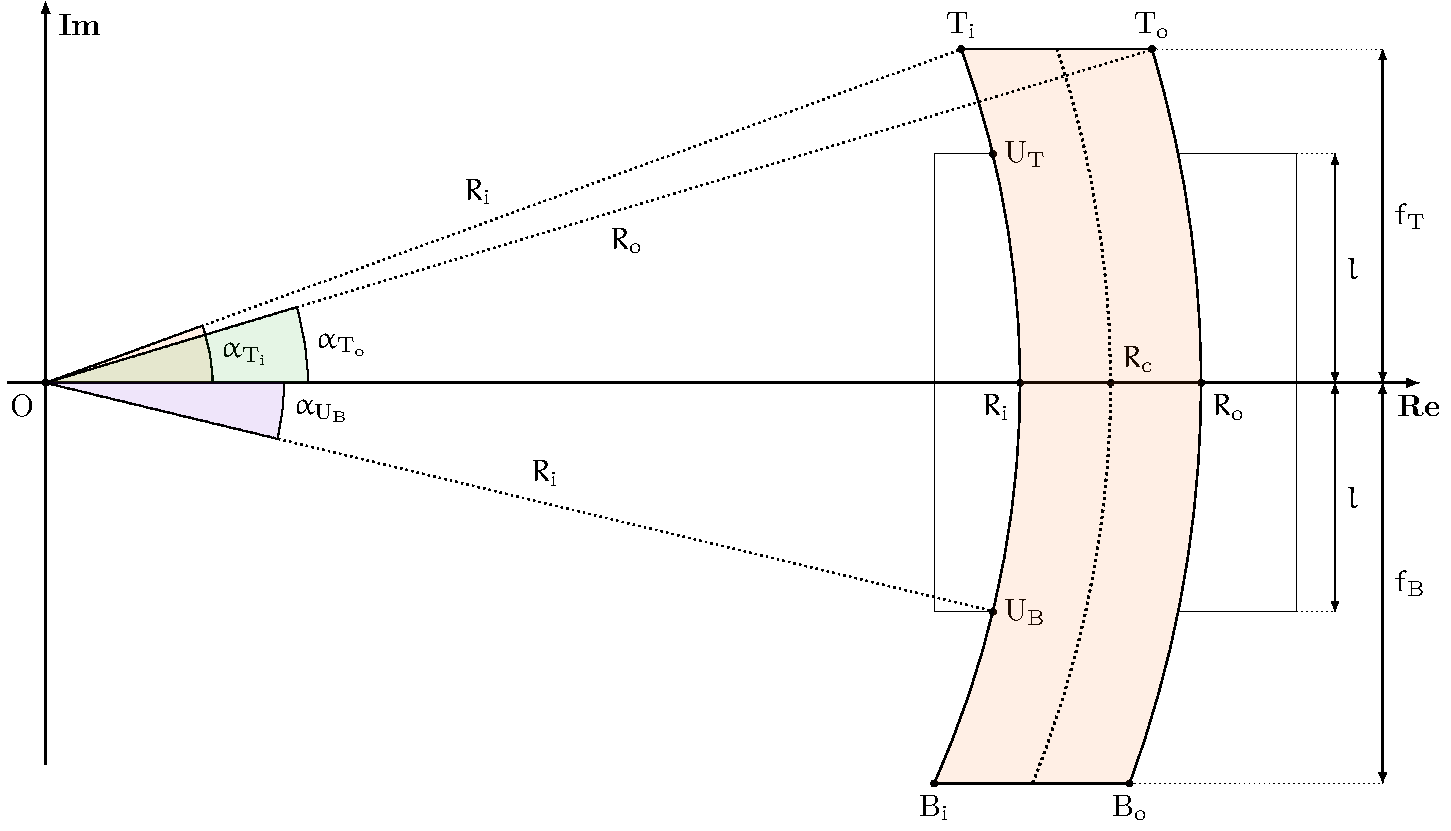
\includegraphics{RfCPN_p5_pictures/mouldoverall.pdf}
\end{adjustbox}
\end{Figlandscape}%
\end{figure}
%%%%%%%%%%%%%%%%%%%%%%%%%%%%%%%%%%%%%%%%%%%%%%%%%%%%%%%%%%
%%%%%%%%%%%%%%%%%%%%%%%%%%%%%%%%%%%%%%%%%%%%%%%%%%%%%%%%%%
%%%%%%%%%%%%%%%%%%%%%%%%%%%%%%%%%%%%%%%%%%%%%%%%%%%%%%%%%%


%%%%%%%%%%%%%%%%%%%%%%%%%%%%%%%%%%%%%%%%%%%%%%%%%%%%%%%%%%
%% subsection 1.1.1 %%%%%%%%%%%%%%%%%%%%%%%%%%%%%%%%%%%%%%
%%%%%%%%%%%%%%%%%%%%%%%%%%%%%%%%%%%%%%%%%%%%%%%%%%%%%%%%%%
\subsection{スペーサを用いた再振分け}
\index{モールド}モールドの\index{わんきょく(モールド)@湾曲(モールド)}湾曲における円の中心\index{O(わんきょくちゅうしん)@O(湾曲中心)}Oを\index{げんてんO@原点O}原点とした\index{ふくそへいめん@複素平面}複素平面を考える
%% footnote %%%%%%%%%%%%%%%%%%%%%
\footnote{ここでは$0 < R_\mathrm c < \infty$ ($0 < \nicefrac1{R_\mathrm c} < \infty$)としている。
$R_\mathrm c \to \infty$ ($\nicefrac1{R_\mathrm c} \to 0$)の場合、すなわち\index{わんきょくのないモールド@湾曲のないモールド}湾曲のないまっすぐなモールドの場合は、別途考える必要がある。}。
%%%%%%%%%%%%%%%%%%%%%%%%%%%%%%%%%
このとき、\pageautoref{fig:mouldOnComplexPlane1}のように、$R_\mathrm c$, $R_\mathrm i$, $R_\mathrm o$, $f_\mathrm T$, $f_\mathrm B$, $l$, $\alpha_{\mathrm T_\mathrm i}$, $\alpha_{\mathrm T_\mathrm o}$, $\alpha_{\mathrm U_\mathrm B}$をとると、
\begin{subequations}
%% label{eq:constraintUpoint1}
%% label{eq:constraintUpoint2}
\begin{gather}
  \label{eq:constraintUpoint1}
  R_\mathrm o - R_\mathrm c = R_\mathrm c - R_\mathrm i = \frac{W_x}2~, \qquad
  \IP\left(R_\mathrm oe^{i\alpha_{\mathrm T_\mathrm o}} - R_\mathrm ie^{i\alpha_{\mathrm T_\mathrm i}}\right)
  = 0~,\\
  \label{eq:constraintUpoint2}
  \sin\alpha_{\mathrm T_\mathrm i} = \frac{f_\mathrm T}{R_\mathrm i}, \qquad
  \sin\alpha_{\mathrm U_\mathrm B} = \frac l{R_\mathrm i}, \qquad
  \tan\theta = \frac{\delta_\mathrm s}{2l}~.
\end{gather}
\end{subequations}
ここで$W_x$はモールドの(AC)外径、$\delta_\mathrm s$は\index{スペーサあつ@スペーサ厚}スペーサの厚さ(\textbf{スペーサ厚})である。
このときモールドを原点Oを中心に$\Omega$だけ回転し、さらに点U$_\mathrm B$($R_\mathrm i$, $-\alpha_{\mathrm U_\mathrm B}$)を中心に$-\theta$だけ回転すると、点T$_\mathrm i$($R_\mathrm i$, $\alpha_{\mathrm T_\mathrm i}$)は、
%% label{eq:afterftUpoint}
\begin{align}
  \notag
  & e^{-i\theta}\left\{R_\mathrm ie^{i(\alpha_{\mathrm T_\mathrm i} + \Omega)} - R_\mathrm ie^{-i\alpha_{\mathrm U_\mathrm B}}\right\}
    +R_\mathrm ie^{-i\alpha_{\mathrm U_\mathrm B}}\\
  &= R_\mathrm i
     \left\{
       e^{i(\alpha_{\mathrm T_\mathrm i} + \Omega - \theta)} - e^{-i(\alpha_{\mathrm U_\mathrm B} + \theta)} + e^{-i\alpha_{\mathrm U_\mathrm B}}
     \right\}
  \label{eq:afterftUpoint}
\end{align}
に移動する。
また同様に点T$_\mathrm o$($R_\mathrm o$, $\alpha_{\mathrm T_\mathrm o}$)は
\begin{align*}
  \notag
  R_\mathrm oe^{i(\alpha_{\mathrm T_\mathrm o} + \Omega - \theta)}
  -R_\mathrm i\left\{e^{-i(\alpha_{\mathrm U_\mathrm B} + \theta)}-e^{-i\alpha_{\mathrm U_\mathrm B}}\right\}
\end{align*}
に移動する。
したがって、これらの差
\begin{align*}
  \notag
  e^{i(\Omega - \theta)}\left(R_\mathrm oe^{i\alpha_{\mathrm T_\mathrm o}} - R_\mathrm ie^{i\alpha_{\mathrm T_\mathrm i}}\right)
\end{align*}
の虚部が0であればよい。
つまり、\pageeqref{eq:constraintUpoint1}より、$\Omega = \theta$である
%% footnote %%%%%%%%%%%%%%%%%%%%%
\footnote{ここでは$0 \leq \Omega, \theta < \nicefrac \pi2$としている。}。
%%%%%%%%%%%%%%%%%%%%%%%%%%%%%%%%%

スペーサを入れた後の(トップ側の)振分長は、\pageeqref{eq:afterftUpoint}の虚部を見ればよい。
\begin{align*}
  R_\mathrm i\left\{\sin\alpha_{\mathrm T_\mathrm i} + \sin(\alpha_{\mathrm U_\mathrm B} + \theta) - \sin\alpha_{\mathrm U_\mathrm B}\right\}
  &= f_\mathrm T -l
     +R_\mathrm i\left(\sin\alpha_{\mathrm U_\mathrm B}\cos\theta + \cos\alpha_{\mathrm U_\mathrm B}\sin\theta\right)\\
  &= f_\mathrm T -l+l\cdot\frac{2l}{\sqrt{4l^2+\delta_\mathrm s^2}}
     +\sqrt{R_\mathrm i^2-l^2}\cdot\frac{\delta_\mathrm s}{\sqrt{4l^2+\delta_\mathrm s^2}}\\
  &= f_\mathrm T -l+\frac{2l^2+\delta_\mathrm s\sqrt{R_\mathrm i^2-l^2}}{\sqrt{4l^2+\delta_\mathrm s^2}}~.
\end{align*}
まとめると、厚さ$\delta_\mathrm s$の\index{スペーサ}スペーサを入れた後のトップ側の\index{ふりわけちょう@振分長}振分長$f'_\mathrm T$は、
\begin{align*}
  f'_\mathrm T
  = f_\mathrm T -l
    +\frac{2l^2+\delta_\mathrm s\sqrt{\left(R_\mathrm c-\nicefrac{W_x}2\right)^2-l^2}}{\sqrt{4l^2+\delta_\mathrm s^2}}~.
\end{align*}


%%%%%%%%%%%%%%%%%%%%%%%%%%%%%%%%%%%%%%%%%%%%%%%%%%%%%%%%%%
%% subsection 1.1.2 %%%%%%%%%%%%%%%%%%%%%%%%%%%%%%%%%%%%%%
%%%%%%%%%%%%%%%%%%%%%%%%%%%%%%%%%%%%%%%%%%%%%%%%%%%%%%%%%%
\subsection{振分長が均等になるスペーサ厚}
%%%%%%%%%%%%%%%%%%%%%%%%%%%%%%%
トップ側とボトム側の\index{きんとうふりわけ@均等振分}振分長が同じになるとき、$\delta_\mathrm s$は
\begin{align*}
  f'_\mathrm T - f_\mathrm T = \frac{f_\mathrm B - f_\mathrm T}2
\end{align*}
を満たす。
これより、
\begin{align*}
  \frac{2l^2+\delta_\mathrm s\sqrt{R_\mathrm i^2-l^2}}{\sqrt{4l^2+\delta_\mathrm s^2}} = l'\qquad
  \left(l' \equiv l + \frac{f_\mathrm B-f_\mathrm T}2\right)
\end{align*}
両辺を2乗すると、
\begin{gather*}
  4l^4+\delta_\mathrm s^2\left(R_\mathrm i^2-l^2\right)+4l^2\delta_\mathrm s\sqrt{R_\mathrm i^2-l^2}
  = l'^2\left(4l^2+\delta_\mathrm s^2\right)\\
  \longrightarrow\quad
  \delta_\mathrm s^2\left(R_\mathrm i^2-l^2-l'^2\right)
  +4l^2\delta_\mathrm s\sqrt{R_\mathrm i^2-l^2} -4l^2\left(l'^2 - l^2\right)
  = 0.
\end{gather*}
$\delta_\mathrm s > 0$より、
\begin{align*}
  \delta_\mathrm s
  &= \frac{\sqrt{4l^4\left(R_\mathrm i^2-l^2\right)
                 +4l^2\left(R_\mathrm i^2-l^2-l'^2\right)\left(l'^2 - l^2\right)}
           -2l^2\sqrt{R_\mathrm i^2-l^2}}{R_\mathrm i^2-l^2-l'^2}\\
  &= 2l\cdot\frac{l'\sqrt{R_\mathrm i^2-l'^2}-l\sqrt{R_\mathrm i^2-l^2}}{R_\mathrm i^2-l^2-l'^2}
\end{align*}
まとめると、求める\index{スペーサあつ@スペーサ厚}スペーサ厚$\delta_\mathrm s$は、
\begin{align*}
  \delta_\mathrm s
  = 2l\cdot
    \frac{\displaystyle
          \left(l+\frac{f_\mathrm B-f_\mathrm T}2\right)
          \sqrt{\left(R_\mathrm c-\frac{W_x}2\right)^2
                -\left(l+\frac{f_\mathrm B-f_\mathrm T}2\right)^2}
          -l\sqrt{\left(R_\mathrm c-\frac{W_x}2\right)^2-l^2}}
         {\displaystyle
          \left(R_\mathrm c-\frac{W_x}2\right)^2-l^2
          -\left(l+\frac{f_\mathrm B-f_\mathrm T}2\right)^2}~.
\end{align*}



\clearpage
%%%%%%%%%%%%%%%%%%%%%%%%%%%%%%%%%%%%%%%%%%%%%%%%%%%%%%%%%%
%% section 20.2 %%%%%%%%%%%%%%%%%%%%%%%%%%%%%%%%%%%%%%%%%%
%%%%%%%%%%%%%%%%%%%%%%%%%%%%%%%%%%%%%%%%%%%%%%%%%%%%%%%%%%
\modHeadsection{受板がある場合}
\index{ジグ}ジグの\index{ワーク}ワークと接する部品(\index{うけいた@受板}\textbf{受板})の大きさを考慮した場合を考える。
ワークに接する側の面は半径$\rho$の円弧(\index{うけいたのけい@受板の径}受板の径), 虚軸方向の厚み(\index{うけいたのはば@受板の幅}受板の幅)は$\sigma$とする。
また受板の虚軸負方向側の面は、ジグのそれと同じ平面上にあるものとする。
%%%%%%%%%%%%%%%%%%%%%%%%%%%%%%%%%%%%%%%%%%%%%%%%%%%%%%%%%%
%% figure %%%%%%%%%%%%%%%%%%%%%%%%%%%%%%%%%%%%%%%%%%%%%%%%
%%%%%%%%%%%%%%%%%%%%%%%%%%%%%%%%%%%%%%%%%%%%%%%%%%%%%%%%%%
\begin{figure}[p]%
\begin{Figbox}[valign=top]%
\resizebox{\linewidth-35pt}{!}{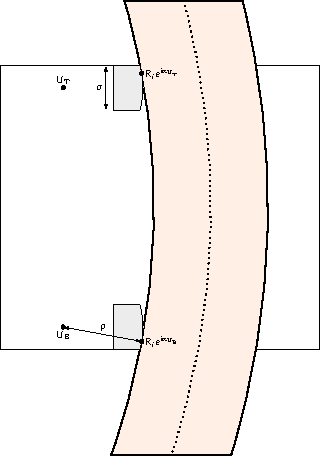
\includegraphics{RfCPN_p5_pictures/mouldUkeita.pdf}}%
\vfill~
\captionof{figure}[受板がある場合]{%
 \index{うけいた@受板}受板がある場合\newline
 $\rho$, $\sigma$は\index{うけいたのけい@受板の径}受板の径および\index{うけいたのはば@受板の幅}受板の幅を示し、U$_\mathrm T$, U$_\mathrm B$はそれぞれの受板の円弧の中心点を示す。
 受板があると\index{ワーク}ワークとの\index{せってん(ワークとうけいた)@接点(ワークと受板)}接点U$_\mathrm B$の位置も変化する。
 なお受板は、トップ側とボトム側で同じものであり、その片面はジグの片面と揃える形で装着されるものとする。
 }%\label{fig:mouldwithukeita}
\end{Figbox}%
\end{figure}%
%%%%%%%%%%%%%%%%%%%%%%%%%%%%%%%%%%%%%%%%%%%%%%%%%%%%%%%%%%
%%%%%%%%%%%%%%%%%%%%%%%%%%%%%%%%%%%%%%%%%%%%%%%%%%%%%%%%%%
%%%%%%%%%%%%%%%%%%%%%%%%%%%%%%%%%%%%%%%%%%%%%%%%%%%%%%%%%%
\index{うけいたのちゅうしん@受板の中心}受板の径の中心を改めてU$_\mathrm B$とし、また\index{げんてんO@原点O}原点Oに対する\index{へんかく(うけいた)@偏角(受板)}偏角を改めて$-\alpha_{\mathrm U_\mathrm B}$とすると、これはU$_\mathrm B$($R_\mathrm i-\rho$, $-\alpha_{\mathrm U_\mathrm B}$)と表すことができる。
ただし、\pageeqref{eq:constraintUpoint2}は以下のようになる。
\begin{align*}
  \sin\alpha_{\mathrm U_\mathrm B} = \frac{\bar l}{R_\mathrm i-\rho}\quad, \quad
  \tan\psi = \frac{\delta_\mathrm s}{2\bar l} \quad
  \left(~\bar l \equiv l-\frac\sigma2~\right).
\end{align*}
これを原点Oを中心に$\Omega$だけ回転し、さらに点U$_\mathrm B$($R_\mathrm i-\rho$, $-\alpha_{\mathrm U_\mathrm B}$)を中心に点T$_\mathrm i$($R_\mathrm i$, $\alpha_{\mathrm T_\mathrm i}$)を$-\theta$だけ回転すると、
%% label{eq:afterftUfinite}
\begin{align}
  \notag
  & e^{-i\theta}\!
    \left\{R_\mathrm ie^{i(\alpha_{\mathrm T_\mathrm i}+\Omega)}
           -R_\mathrm i'e^{-i\alpha_{\mathrm U_\mathrm B}}\right\}
    +R_\mathrm i'e^{-i\alpha_{\mathrm U_\mathrm B}}\\
  & = R_\mathrm ie^{i(\alpha_{\mathrm T_\mathrm i}+\Omega-\theta)}
      -R_\mathrm i'\!
       \left\{e^{-i(\alpha_{\mathrm U_\mathrm B}+\theta)}-e^{-i\alpha_{\mathrm U_\mathrm B}}\right\}\qquad
    \big(R_\mathrm i' \equiv R_\mathrm i-\rho\big)
    \label{eq:afterftUfinite}
\end{align}
に移動する。
同様に点T$_\mathrm o$($R_\mathrm o$, $\alpha_{\mathrm T_\mathrm o}$)は
\begin{align*}
  R_\mathrm oe^{i(\alpha_{\mathrm T_\mathrm o}+\Omega-\theta)}
  -R_\mathrm i'\!
   \left\{e^{-i(\alpha_{\mathrm U_\mathrm B} + \theta)} - e^{-i\alpha_{\mathrm U_\mathrm B}}\right\}
\end{align*}
に移動する。
したがって、これらの差
\begin{align*}
  e^{i(\Omega-\theta)}
  \left(R_\mathrm oe^{i\alpha_{\mathrm T_\mathrm o}} - R_\mathrm ie^{i\alpha_{\mathrm T_\mathrm i}}\right)
\end{align*}
の虚部が0であればよい。
つまり、\pageeqref{eq:constraintUpoint1}より、受板がある場合も$\Omega = \theta$である。


%%%%%%%%%%%%%%%%%%%%%%%%%%%%%%%%%%%%%%%%%%%%%%%%%%%%%%%%%%
%% subsection 20.2.1 %%%%%%%%%%%%%%%%%%%%%%%%%%%%%%%%%%%%%
%%%%%%%%%%%%%%%%%%%%%%%%%%%%%%%%%%%%%%%%%%%%%%%%%%%%%%%%%%
\subsection{受板の接点}
\index{うけいた@受板}受板とワークとの(トップ側の)接点は、$R_\mathrm ie^{i\alpha_{\mathrm U_\mathrm B}}$で与えられる。
このとき厚さ$\delta_\mathrm s$のスペーサを取付けると、U$_\mathrm B$を中心に回転するが、それに伴い\index{ワークとジグのせってん@ワークとジグの接点}受板との接点の位置も変化する。

%%%%%%%%%%%%%%%%%%%%%%%%%%%%%%%%%%%%%%%%%%%%%%%%%%%%%%%%%%
%% subsubsection 19.2.1.1 %%%%%%%%%%%%%%%%%%%%%%%%%%%%%%%%
%%%%%%%%%%%%%%%%%%%%%%%%%%%%%%%%%%%%%%%%%%%%%%%%%%%%%%%%%%
\subsubsection{回転後のモールドの湾曲中心}
%%%%%%%%%%%%%%%%%%%%%%%%%
厚さ$\delta_\mathrm s$の\index{スペーサ}スペーサを挟むと、トップ側における\index{うけいたのちゅうしん@受板の中心}受板の円の中心U$_\mathrm B$は実軸方向に$\delta_\mathrm s$だけ移動するので、
\begin{align*}
  R_\mathrm i'e^{i\alpha_{\mathrm U_\mathrm B}}
  \quad\longrightarrow\quad
  \delta_\mathrm s+R_\mathrm i'e^{i\alpha_{\mathrm U_\mathrm B}}\ .
\end{align*}
よって、それぞれの受板の中心U$_\mathrm B$, U$_\mathrm T$を結んだ線分U$_\mathrm B$U$_\mathrm T$は、U$_\mathrm B$を中心に$-\psi$だけ傾いた線分U$_\mathrm B'$U$_\mathrm T'$となる
%% footnote %%%%%%%%%%%%%%%%%%%%%
\footnote{%
U$_\mathrm B'$U$_\mathrm T'$の長さは$\bar l\sec\psi$であり、U$_\mathrm B$U$_\mathrm T$の長さ$\bar l$より長くなることに注意。}。
%%%%%%%%%%%%%%%%%%%%%%%%%%%%%%%%%
\index{かいてんごのわんきょくちゅうしん@回転後の湾曲中心}回転後のワークの湾曲中心は、この線分の垂直二等分線上にあり、またそれぞれの受板の中心から$R_\mathrm i'$の距離の位置にある。
つまり、この傾いた線分U$_\mathrm B'$U$_\mathrm T'$の中点から、角度$\pi-\psi$, 大きさ$\sqrt{R_\mathrm i'^2-\frac{\delta_\mathrm s^2+(2\bar l)^2}4}$の位置に移動する。
したがって、回転後における湾曲中心O$'$は、
%% label{eq:afterOrgin}
\begin{align}
  \notag
  & \frac{\delta_\mathrm s}2+\sqrt{R_\mathrm i'^2-\bar l^2}
    +\sqrt{R_\mathrm i'^2-\frac{\delta_\mathrm s^2+(2\bar l)^2}4}e^{i(\pi-\psi)}\\
  & = \frac{\delta_\mathrm s}2+\sqrt{R_\mathrm i'^2-\bar l^2}-\sqrt{R_\mathrm i'^2-\frac{\delta_\mathrm s^2+(2\bar l)^2}4}\cos\psi
      +i\sqrt{R_\mathrm i'^2-\frac{\delta_\mathrm s^2+(2\bar l)^2}4}\sin\psi\ .
    \label{eq:afterOrgin}
\end{align}

\clearpage
%%%%%%%%%%%%%%%%%%%%%%%%%%%%%%%%%%%%%%%%%%%%%%%%%%%%%%%%%%
%% subsubsection 19.2.1.2 %%%%%%%%%%%%%%%%%%%%%%%%%%%%%%%%
%%%%%%%%%%%%%%%%%%%%%%%%%%%%%%%%%%%%%%%%%%%%%%%%%%%%%%%%%%
\subsubsection{回転後の接点(トップ側)}
\index{かいてんごのうけいたのちゅうしん@回転後の受板の中心}回転後のトップ側における受板の中心U$_\mathrm T'$と\index{かいてんごのわんきょくちゅうしん@回転後の湾曲中心}湾曲中心O$'$との差をとると、
\begin{align*}
  \frac{\delta_\mathrm s}2+\sqrt{R_\mathrm i'^2-\frac{\delta_\mathrm s^2+(2\bar l)^2}4}\cos\psi
  +i\left\{\bar l-\sqrt{R_\mathrm i'^2-\frac{\delta_\mathrm s^2+(2\bar l)^2}4}\sin\psi\right\}
  = R_\mathrm i'e^{i\alpha'_{\mathrm U_\mathrm T}}\ .
\end{align*}
ここで、
\begin{align*}
  \tan\alpha'_{\mathrm U_\mathrm T}
  = \frac{\displaystyle\bar l-\sqrt{R_\mathrm i'^2-\frac{\delta_\mathrm s^2+(2\bar l)^2}4}\sin\psi}
         {\displaystyle\frac{\delta_\mathrm s}2+\sqrt{R_\mathrm i'^2-\frac{\delta_\mathrm s^2+(2\bar l)^2}4}\cos\psi}\ .
\end{align*}
%%%%%%%%%%%%%%%%%%%%%%%%%%%%%%%%%%%%%%%%%%%%%%%%%%%%%%%%%%
%% hosoku %%%%%%%%%%%%%%%%%%%%%%%%%%%%%%%%%%%%%%%%%%%%%%%%
%%%%%%%%%%%%%%%%%%%%%%%%%%%%%%%%%%%%%%%%%%%%%%%%%%%%%%%%%%
\begin{hosoku}
これの大きさは、$\delta_\mathrm s\cos\psi-2\bar l\sin\psi = 0$より、
\begin{align*}
  \left\{\frac{\delta_\mathrm s}2+\sqrt{R_\mathrm i'^2-\frac{\delta_\mathrm s^2+(2\bar l)^2}4}\cos\psi\right\}^2
  +\left\{\bar l-\sqrt{R_\mathrm i'^2-\frac{\delta_\mathrm s^2+(2\bar l)^2}4}\sin\psi\right\}^2
  = R_\mathrm i'^2\ .
\end{align*}
\end{hosoku}
%%%%%%%%%%%%%%%%%%%%%%%%%%%%%%%%%%%%%%%%%%%%%%%%%%%%%%%%%%
%%%%%%%%%%%%%%%%%%%%%%%%%%%%%%%%%%%%%%%%%%%%%%%%%%%%%%%%%%
%%%%%%%%%%%%%%%%%%%%%%%%%%%%%%%%%%%%%%%%%%%%%%%%%%%%%%%%%%
よって、回転後の接点は以下で与えられる。
\begin{align*}
  &  R_\mathrm ie^{i\alpha'_{\mathrm U_\mathrm T}}
     +\frac{\delta_\mathrm s}2+\sqrt{R_\mathrm i'^2-\bar l^2}-\sqrt{R_\mathrm i'^2-\frac{\delta_\mathrm s^2+(2\bar l)^2}4}\cos\psi
     +i\sqrt{R_\mathrm i'^2-\frac{\delta_\mathrm s^2+(2\bar l)^2}4}\sin\psi\\
  &= \delta_\mathrm s+R_\mathrm i'e^{i\alpha_{\mathrm U_\mathrm B}}+\rho e^{i\alpha'_{\mathrm U_\mathrm T}}\ .
\end{align*}

%%%%%%%%%%%%%%%%%%%%%%%%%%%%%%%%%%%%%%%%%%%%%%%%%%%%%%%%%%
%% subsubsection 1.2.1.3 %%%%%%%%%%%%%%%%%%%%%%%%%%%%%%%%%
%%%%%%%%%%%%%%%%%%%%%%%%%%%%%%%%%%%%%%%%%%%%%%%%%%%%%%%%%%
\subsubsection{回転後の接点(ボトム側)}
回転後のボトム側における受板の中心U$_\mathrm B$と\index{わんきょくちゅうしん@湾曲中心}湾曲中心O$'$との差をとると、
\begin{align*}
  -\frac{\delta_\mathrm s}2+\sqrt{R_\mathrm i'^2-\frac{\delta_\mathrm s^2+(2\bar l)^2}4}\cos\psi
  -i\left\{\bar l+\sqrt{R_\mathrm i'^2-\frac{\delta_\mathrm s^2+(2\bar l)^2}4}\sin\psi\right\}
  = R_\mathrm i'e^{-i\alpha'_{\mathrm U_\mathrm B}}
\end{align*}
ここで、
\begin{align*}
  \tan\alpha'_{\mathrm U_\mathrm B}
  = \frac{\displaystyle\bar l+\sqrt{R_\mathrm i'^2-\frac{\delta_\mathrm s^2+(2\bar l)^2}4}\sin\psi}
         {\displaystyle-\frac{\delta_\mathrm s}2+\sqrt{R_\mathrm i'^2-\frac{\delta_\mathrm s^2+(2\bar l)^2}4}\cos\psi}
\end{align*}
よって、回転後の接点は以下で与えられる。
%% label{eq:afterUBcontact}
\begin{align}
  \notag
  &  R_\mathrm ie^{-i\alpha'_{\mathrm U_\mathrm B}}
     +\frac{\delta_\mathrm s}2+\sqrt{R_\mathrm i'^2-\bar l^2}-\sqrt{R_\mathrm i'^2-\frac{\delta_\mathrm s^2+(2\bar l)^2}4}\cos\psi
     +i\sqrt{R_\mathrm i'^2-\frac{\delta_\mathrm s^2+(2\bar l)^2}4}\sin\psi\\
  &= R_\mathrm i'e^{-i\alpha_{\mathrm U_\mathrm B}}+\rho e^{-i\alpha'_{\mathrm U_\mathrm B}}
   \label{eq:afterUBcontact}
\end{align}
%%%%%%%%%%%%%%%%%%%%%%%%%%%%%%%%%%%%%%%%%%%%%%%%%%%%%%%%%%
%% hosoku %%%%%%%%%%%%%%%%%%%%%%%%%%%%%%%%%%%%%%%%%%%%%%%%
%%%%%%%%%%%%%%%%%%%%%%%%%%%%%%%%%%%%%%%%%%%%%%%%%%%%%%%%%%
\begin{hosoku}
辺の長さが$R_i'$, $R_i'$, $2\bar l$の二等辺三角形$\triangle$OU$_\mathrm B$U$_\mathrm T$の部分が、回転後には辺の長さ$R_i'$, $R_i'$, $\sqrt{\delta_\mathrm s^2+(2\bar l)^2}$の二等辺三角形$\triangle$O$'$U$_\mathrm B'$U$_\mathrm T'$となる。
実際、$\cos2a = 1-2\sin^2\!a$より、
\begin{align*}
  \sin^2\frac{\alpha'_{\mathrm U_\mathrm T}+\alpha'_{\mathrm U_\mathrm B}}2
  = \frac{\delta_\mathrm s^2+(2\bar l)^2}{4R_\mathrm i'^2}\ .
\end{align*}
\end{hosoku}
%%%%%%%%%%%%%%%%%%%%%%%%%%%%%%%%%%%%%%%%%%%%%%%%%%%%%%%%%%
%%%%%%%%%%%%%%%%%%%%%%%%%%%%%%%%%%%%%%%%%%%%%%%%%%%%%%%%%%
%%%%%%%%%%%%%%%%%%%%%%%%%%%%%%%%%%%%%%%%%%%%%%%%%%%%%%%%%%


%%%%%%%%%%%%%%%%%%%%%%%%%%%%%%%%%%%%%%%%%%%%%%%%%%%%%%%%%%
%% subsection 1.2.2 %%%%%%%%%%%%%%%%%%%%%%%%%%%%%%%%%%%%%%
%%%%%%%%%%%%%%%%%%%%%%%%%%%%%%%%%%%%%%%%%%%%%%%%%%%%%%%%%%
\subsection{スペーサによるモールドの回転角}
厚さ$\delta_\mathrm s$の\index{スペーサ}スペーサを挿入すると、\index{わんきょくちゅうしん@湾曲中心}湾曲中心Oは、U$_\mathrm B$を中心に$-\left(\alpha'_{\mathrm U_\mathrm B}\!-\alpha_{\mathrm U_\mathrm B}\right)$だけ回転する。
実際、
\begin{align*}
  -R_\mathrm i'e^{-i\alpha'_{\mathrm U_\mathrm B}}+R_\mathrm i'e^{-i\alpha_{\mathrm U_\mathrm B}}
  &= R_\mathrm i'(\cos\alpha_{\mathrm U_\mathrm B}-\cos\alpha'_{\mathrm U_\mathrm B})
     +iR_\mathrm i'(\sin\alpha'_{\mathrm U_\mathrm B}-\sin\alpha_{\mathrm U_\mathrm B})
\end{align*}
であり、これは\index{かいてんごのわんきょくちゅうしん@回転後の湾曲中心}回転後の湾曲中心\pageeqref{eq:afterOrgin}に一致する。
つまり、$\alpha'_{\mathrm U_\mathrm B}\!-\alpha_{\mathrm U_\mathrm B}$が$\theta$に相当する。
%%%%%%%%%%%%%%%%%%%%%%%%%%%%%%%%%%%%%%%%%%%%%%%%%%%%%%%%%%
%% hosoku %%%%%%%%%%%%%%%%%%%%%%%%%%%%%%%%%%%%%%%%%%%%%%%%
%%%%%%%%%%%%%%%%%%%%%%%%%%%%%%%%%%%%%%%%%%%%%%%%%%%%%%%%%%
\begin{hosoku}
トップ側の接点U$_\mathrm T'$とボトム側の接点U$_\mathrm B'$の差をとると、
\begin{align*}
  R_\mathrm i\left(e^{i\alpha_{\mathrm U_\mathrm T}'}-e^{-i\alpha'_{\mathrm U_\mathrm B}}\right)
  &= \frac{R_\mathrm i'+\rho}{R_\mathrm i'}\left\{\delta_\mathrm s+i(2\bar l)\right\}
   = \frac{R_\mathrm i}{R_\mathrm i'}\sqrt{\delta_\mathrm s^2+(2\bar l)^2}e^{i(\nicefrac\pi2-\psi)}\ .
\end{align*}
したがって、厚さ$\delta_\mathrm s$のスペーサを挿入すると、両接点を通る直線は$-\psi$だけ傾くことがわかる。
また、その長さは受板中心間U$_\mathrm T'$U$_\mathrm B'$の距離$\sqrt{\delta_\mathrm s^2+(2\bar l)^2}$の$\nicefrac{R_i}{R_i'}$倍になっていることも確かめられる。
\end{hosoku}
%%%%%%%%%%%%%%%%%%%%%%%%%%%%%%%%%%%%%%%%%%%%%%%%%%%%%%%%%%
%%%%%%%%%%%%%%%%%%%%%%%%%%%%%%%%%%%%%%%%%%%%%%%%%%%%%%%%%%
%%%%%%%%%%%%%%%%%%%%%%%%%%%%%%%%%%%%%%%%%%%%%%%%%%%%%%%%%%


%%%%%%%%%%%%%%%%%%%%%%%%%%%%%%%%%%%%%%%%%%%%%%%%%%%%%%%%%%
%% subsection 1.2.3 %%%%%%%%%%%%%%%%%%%%%%%%%%%%%%%%%%%%%%
%%%%%%%%%%%%%%%%%%%%%%%%%%%%%%%%%%%%%%%%%%%%%%%%%%%%%%%%%%
\subsection{スペーサによる再振分け}

%%%%%%%%%%%%%%%%%%%%%%%%%%%%%%%%%%%%%%%%%%%%%%%%%%%%%%%%%%
%% subsubsection 1.2.3.1 %%%%%%%%%%%%%%%%%%%%%%%%%%%%%%%%%
%%%%%%%%%%%%%%%%%%%%%%%%%%%%%%%%%%%%%%%%%%%%%%%%%%%%%%%%%%
\subsubsection{再振分長}
\index{スペーサ}スペーサを入れた後のトップ側の\index{ふりわけちょう@振分長}振分長(\index{さいふりわけちょう@再振分長}\textbf{再振分長})$f'_\mathrm T$は、\pageeqref{eq:afterftUfinite}の虚部を見ればよい。
回転角は$-(\alpha'_{\mathrm U_\mathrm B}-\alpha_{\mathrm U_\mathrm B})$なので、
\begin{align*}
  f'_\mathrm T
  = R_\mathrm i\sin\alpha_{\mathrm T_\mathrm i}
    +R_\mathrm i'\left(\sin\alpha'_{\mathrm U_\mathrm B}-\sin\alpha_{\mathrm U_\mathrm B}\right)
  &= f_\mathrm T+\sqrt{R_\mathrm i'^2-\frac{\delta_\mathrm s^2+(2\bar l)^2}4}\sin\psi\\
  &= f_\mathrm T+\sqrt{R_\mathrm i'^2-\frac{\delta_\mathrm s^2+(2\bar l)^2}4}\frac{\delta_\mathrm s}{\sqrt{\delta_\mathrm s^2+(2\bar l)^2}}\ .
\end{align*}

%%%%%%%%%%%%%%%%%%%%%%%%%%%%%%%%%%%%%%%%%%%%%%%%%%%%%%%%%%
%% subsubsection 1.2.3.2 %%%%%%%%%%%%%%%%%%%%%%%%%%%%%%%%%
%%%%%%%%%%%%%%%%%%%%%%%%%%%%%%%%%%%%%%%%%%%%%%%%%%%%%%%%%%
\subsubsection{モールドの移動距離}
\pageeqref{eq:afterftUfinite}の実部は、
\begin{align*}
  & R_\mathrm i\cos\alpha_{\mathrm T_\mathrm i}
    -R_\mathrm i'(\cos\alpha'_{\mathrm U_\mathrm B}-\cos\alpha_{\mathrm U_\mathrm B})\\
  & = \sqrt{R_\mathrm i^2-f_\mathrm T^2}+\frac{\delta_\mathrm s}2+\sqrt{R_\mathrm i'^2-\bar l^2}
      -\sqrt{R_\mathrm i'^2-\frac{\delta_\mathrm s^2+(2\bar l)^2}4}\cos\psi
\end{align*}
となる。
よって、\index{スペーサ}スペーサを挿入することにより、ワークは水平・鉛直方向にそれぞれ、
\begin{subequations}
%% label{eq:spacerMoveHdistance}
\begin{alignat}{2}
  \label{eq:spacerMoveHdistance}
  \text{水平方向:}\quad
  & \frac{\delta_\mathrm s}2+\sqrt{R_\mathrm i'^2-\bar l^2}-\sqrt{R_\mathrm i'^2-\frac{\delta_\mathrm s^2+(2\bar l)^2}4}\frac{2\bar l}{\sqrt{\delta_\mathrm s^2+(2\bar l)^2}}\\
  \text{鉛直方向:}\quad
  & \sqrt{R_\mathrm i'^2-\frac{\delta_\mathrm s^2+(2\bar l)^2}4}\frac{\delta_\mathrm s}{\sqrt{\delta_\mathrm s^2+(2\bar l)^2}}
\end{alignat}
\end{subequations}
だけ移動することがわかる。


%\clearpage
%%%%%%%%%%%%%%%%%%%%%%%%%%%%%%%%%%%%%%%%%%%%%%%%%%%%%%%%%%
%% subsection 1.2.4 %%%%%%%%%%%%%%%%%%%%%%%%%%%%%%%%%%%%%%
%%%%%%%%%%%%%%%%%%%%%%%%%%%%%%%%%%%%%%%%%%%%%%%%%%%%%%%%%%
\subsection{再振分長が均等になるスペーサ厚}
トップ側とボトム側の\index{きんとうふりわけ@均等振分}振分長が同じになるとき、$\delta_\mathrm s$は
\begin{align*}
  \sqrt{R_\mathrm i'^2-\frac{\delta_\mathrm s^2+(2\bar l)^2}4}\frac{\delta_\mathrm s}{\sqrt{\delta_\mathrm s^2+(2\bar l)^2}} = f_d \qquad
  \left(f_d \equiv \frac{f_\mathrm B-f_\mathrm T}2\right)\ .
\end{align*}
を満たす。
両辺を2乗して$-4$倍すると、
\begin{align*}
  \delta_\mathrm s^2\left\{\delta_\mathrm s^2+(2\bar l)^2-4R_\mathrm i'^2\right\}+4f_d^2\left\{\delta_\mathrm s^2+(2\bar l)^2\right\}
  & = \delta_\mathrm s^4-2\left\{2R_\mathrm i'^2-2\bar l^2-2f_d^2\right\}\delta_\mathrm s^2+4f_d^2(2\bar l)^2\\
  & = 0\ .
\end{align*}
したがって、$f_\mathrm T = f_\mathrm B$ ($f_d = 0$)のとき$\delta_\mathrm s = 0$であることを考慮して、
\begin{align*}
  \delta_\mathrm s^2
  &= 2\left\{
       R_\mathrm i'^2-\bar l^2-f_d^2-\sqrt{\left(R_\mathrm i'^2-\bar l^2-f_d^2\right)^2-4f_d^2\bar l^2}\,
     \right\}\\
  &= \left(\sqrt{R_\mathrm i'^2-(\bar l-f_d)^2}-\sqrt{R_\mathrm i'^2-(\bar l+f_d)^2}\,\right)^2.
\end{align*}
なお、これはワークが水平・鉛直方向にそれぞれ、
\begin{align*}
  \text{水平方向:}~\frac{\delta_\mathrm s}2+\sqrt{R_\mathrm i^2-\bar l^2}-\frac{2\bar l}{\delta_\mathrm s}f_d\quad(\delta_\mathrm s>0)\ , \qquad
  \text{鉛直方向:}~\frac{f_\mathrm B-f_\mathrm T}2
\end{align*}
だけ移動することを意味する。
%%%%%%%%%%%%%%%%%%%%%%%%%%%%%%%%%%%%%%%%%%%%%%%%%%%%%%%%%%
%% hosoku %%%%%%%%%%%%%%%%%%%%%%%%%%%%%%%%%%%%%%%%%%%%%%%%
%%%%%%%%%%%%%%%%%%%%%%%%%%%%%%%%%%%%%%%%%%%%%%%%%%%%%%%%%%
\begin{hosoku}
改めてまとめると、厚さ$\delta_\mathrm s$のスペーサを(トップ側に)挿入した後の\index{トップふりわけちょう@トップ振分長}トップ側の振分長$f_\mathrm T'$は、
\begin{align*}
  f_\mathrm T'
  = f_\mathrm T+\sqrt{R_\mathrm i'^2-\frac{\delta_\mathrm s^2+(2\bar l)^2}4}\frac{\delta_\mathrm s}{\sqrt{\delta_\mathrm s^2+(2\bar l)^2}}\ .
\end{align*}
トップ側とボトム側の\index{きんとうふりわけ@均等振分}振分長が均等になるときの\index{スペーサあつ@スペーサ厚}スペーサ厚$\delta_\mathrm s'$は、
\begin{align*}
  \delta_\mathrm s' = \sqrt{R_\mathrm i'^2-(\bar l-f_d)^2}-\sqrt{R_\mathrm i'^2-(\bar l+f_d)^2}\ .
\end{align*}
ここで、
\begin{align*}
  R_\mathrm i' = R_\mathrm c-\frac{W_x}2-\rho\ ,\quad
  \bar l = l-\frac\sigma2\ ,\quad
  f_d = \frac{f_\mathrm B-f_\mathrm T}2\ .
\end{align*}
\end{hosoku}
%%%%%%%%%%%%%%%%%%%%%%%%%%%%%%%%%%%%%%%%%%%%%%%%%%%%%%%%%%
%%%%%%%%%%%%%%%%%%%%%%%%%%%%%%%%%%%%%%%%%%%%%%%%%%%%%%%%%%
%%%%%%%%%%%%%%%%%%%%%%%%%%%%%%%%%%%%%%%%%%%%%%%%%%%%%%%%%%



\clearpage
%%%%%%%%%%%%%%%%%%%%%%%%%%%%%%%%%%%%%%%%%%%%%%%%%%%%%%%%%%
%% section 21.3 %%%%%%%%%%%%%%%%%%%%%%%%%%%%%%%%%%%%%%%%%%
%%%%%%%%%%%%%%%%%%%%%%%%%%%%%%%%%%%%%%%%%%%%%%%%%%%%%%%%%%
\modHeadsection{テーブルの回転による振分長の調節}
これまでトップ・ボトム振分長の差を小さくするために\index{スペーサ}スペーサを用いる手法を考えてきた。
スペーサを取付けることは、本質的にはボトム側の\index{うけいた@受板}受板の点U$_\mathrm B$を中心に回転しているということである。
このとき回転の中心はU$_\mathrm B$である必要はなく、他の点でも問題ない。
したがって、スペーサを用いて回転をしなくても、\index{テーブル}テーブルそのものを回転するという手法が考えられる。
これは回転の中心が、受板の点U$_\mathrm B$から\index{テーブルちゅうしん@テーブル中心}\textbf{テーブル中心}Pに変わることに相当する。

\index{うけいたのちゅうしん@受板の中心}受板の中心U$_\mathrm B$と、テーブル中心Pとの実軸方向の距離を$\Delta$とすると、テーブル中心Pの$X$座標$\Delta'$は次で与えられる。
%% label{eq:tableCenter}
\begin{align}
  \label{eq:tableCenter}
  \Delta'
  = \Delta+R_\mathrm i'\cos\alpha_{\mathrm U_\mathrm B} = \Delta+\sqrt{R_\mathrm i'^2-\bar l^2}\ .
\end{align}
\index{トップがわのCがわそとたんてん@トップ側のC側外端点}トップ側のC側外端点T$_\mathrm i$($R_\mathrm i$, $\alpha_{\mathrm T_\mathrm i}$)を、原点Oを中心に$\Omega$だけ回転し、さらに点P\,($\Delta'$, $0$)を中心に$-\theta$だけ回転すると、
\begin{align}
  \label{eq:afterfttable}
  e^{-i\theta}\left\{R_\mathrm i^{i(\alpha_{\mathrm T_\mathrm i}+\Omega)}-\Delta'\right\}+\Delta'
  = R_\mathrm ie^{i(\alpha_{\mathrm T_\mathrm i}+\Omega-\theta)}+\Delta'\left(1-e^{-i\theta}\right)
\end{align}
に移動する。
同様に、\index{トップがわのAがわそとたんてん@トップ側のA側外端点}トップ側のA側外端点T$_\mathrm o$($R_\mathrm o$, $\alpha_{\mathrm T_\mathrm o}$)は、
\begin{align*}
  e^{-i\theta}\!\left\{R_\mathrm o^{i(\alpha_{\mathrm T_\mathrm o}+\Omega)}-\Delta'\right\}+\Delta'
  = R_\mathrm ie^{i(\alpha_{\mathrm T_\mathrm o}+\Omega-\theta)}+\Delta'\!\left(1-e^{-i\theta}\right)
\end{align*}
に移動する。
したがって、これらの差
\begin{align*}
  e^{i(\Omega-\theta)}
  \left(R_\mathrm oe^{i\alpha_{\mathrm T_\mathrm o}}-R_\mathrm ie^{i\alpha_{\mathrm T_\mathrm i}}\right)
\end{align*}
の虚部が$0$であればよい。
よって\pageeqref{eq:constraintUpoint1}より、この場合も$\Omega = \theta$となる。


%%%%%%%%%%%%%%%%%%%%%%%%%%%%%%%%%%%%%%%%%%%%%%%%%%%%%%%%%%
%% subsection 21.3.1 %%%%%%%%%%%%%%%%%%%%%%%%%%%%%%%%%%%%%
%%%%%%%%%%%%%%%%%%%%%%%%%%%%%%%%%%%%%%%%%%%%%%%%%%%%%%%%%%
\subsection{回転後のモールドの湾曲中心および受板との接点}

%%%%%%%%%%%%%%%%%%%%%%%%%%%%%%%%%%%%%%%%%%%%%%%%%%%%%%%%%%
%% subsubsection 21.3.1.1 %%%%%%%%%%%%%%%%%%%%%%%%%%%%%%%%
%%%%%%%%%%%%%%%%%%%%%%%%%%%%%%%%%%%%%%%%%%%%%%%%%%%%%%%%%%
\subsubsection{回転後のモールドの湾曲中心}
\index{かいてんごのわんきょくちゅうしん@回転後の湾曲中心}回転後の湾曲中心O$'$は、点Pを中心に$-\theta$だけ回転するので、
\begin{align*}
  \Delta'\!\left(1-e^{-i\theta}\right) = \Delta'(1-\cos\theta)+i\Delta'\sin\theta\ .
\end{align*}

%%%%%%%%%%%%%%%%%%%%%%%%%%%%%%%%%%%%%%%%%%%%%%%%%%%%%%%%%%
%% subsubsection 21.3.1.2 %%%%%%%%%%%%%%%%%%%%%%%%%%%%%%%%
%%%%%%%%%%%%%%%%%%%%%%%%%%%%%%%%%%%%%%%%%%%%%%%%%%%%%%%%%%
\subsubsection{回転後の接点}
回転後におけるトップ側の\index{ワークとうけいたのせってん@ワークと受板の接点}受板との接点は、点Pを中心に$-\theta$だけ回転するので、
\begin{align*}
  &  e^{-i\theta}\left(R_\mathrm ie^{i\alpha_{\mathrm U_\mathrm B}}-\Delta'\right)+\Delta'\\
  &= R_\mathrm ie^{i(\alpha_{\mathrm U_\mathrm B}-\theta)}+\Delta'\!\left(1-e^{-i\theta}\right)\\
  &= R_\mathrm i\cos(\alpha_{\mathrm U_\mathrm B}-\theta)+\Delta'(1-\cos\theta)
     +i\left\{R_\mathrm i\sin(\alpha_{\mathrm U_\mathrm B}-\theta)+i\Delta'\sin\theta\right\}\ .
\end{align*}
同様に、ボトム側の受板との接点は、
\begin{align*}
  &  e^{-i\theta}\left(R_\mathrm ie^{-i\alpha_{\mathrm U_\mathrm B}}-\Delta'\right)+\Delta'\\
  &= R_\mathrm ie^{-i(\alpha_{\mathrm U_\mathrm B}+\theta)}+\Delta'\!\left(1-e^{-i\theta}\right)\\
  &= R_\mathrm i\cos(\alpha_{\mathrm U_\mathrm B}+\theta)+\Delta'(1-\cos\theta)
     -i\left\{R_\mathrm i\sin(\alpha_{\mathrm U_\mathrm B}+\theta)-i\Delta'\sin\theta\right\}\ .
\end{align*}
%%%%%%%%%%%%%%%%%%%%%%%%%%%%%%%%%%%%%%%%%%%%%%%%%%%%%%%%%%
%% hosoku %%%%%%%%%%%%%%%%%%%%%%%%%%%%%%%%%%%%%%%%%%%%%%%%
%%%%%%%%%%%%%%%%%%%%%%%%%%%%%%%%%%%%%%%%%%%%%%%%%%%%%%%%%%
\begin{hosoku}
両接点との差をとると、
\begin{align*}
  2R_\mathrm i\sin\alpha_{\mathrm U_\mathrm B}\sin\theta+2iR_\mathrm i\sin\alpha_{\mathrm U_\mathrm B}\cos\theta
  = \frac{R_\mathrm i}{R_\mathrm i'}(2\bar l)e^{i(\pi-\theta)}
\end{align*}
となり、\index{うけいたのちゅうしん@受板の中心}受板の両中心間(長さ$2\bar l$)を結んだ線分を$\nicefrac{R_\mathrm i}{R_\mathrm i'}$倍し、虚軸から$-\theta$だけ傾けたものになっていることがわかる。
\end{hosoku}
%%%%%%%%%%%%%%%%%%%%%%%%%%%%%%%%%%%%%%%%%%%%%%%%%%%%%%%%%%
%%%%%%%%%%%%%%%%%%%%%%%%%%%%%%%%%%%%%%%%%%%%%%%%%%%%%%%%%%
%%%%%%%%%%%%%%%%%%%%%%%%%%%%%%%%%%%%%%%%%%%%%%%%%%%%%%%%%%


%%%%%%%%%%%%%%%%%%%%%%%%%%%%%%%%%%%%%%%%%%%%%%%%%%%%%%%%%%
%% subsection 21.3.2 %%%%%%%%%%%%%%%%%%%%%%%%%%%%%%%%%%%%%
%%%%%%%%%%%%%%%%%%%%%%%%%%%%%%%%%%%%%%%%%%%%%%%%%%%%%%%%%%
\subsection{回転後の振分長}
回転後の\index{トップさいふりわけちょう@トップ再振分長}トップ側の振分長$f_\mathrm T'$は、\pageeqref{eq:afterfttable}の虚部を見ればよいので、
\begin{subequations}
%\label{eq:saifuriwake}
\begin{align}
  \label{eq:saifuriwakeT}
  f_\mathrm T'
  = f_\mathrm T+\Delta'\sin\theta
  = f_\mathrm T+\left(\Delta+\sqrt{R_\mathrm i'-\bar l^2}\right)\sin\theta\ .
\end{align}
同様に、\index{ボトムさいふりわけちょう@ボトム再振分長}ボトムの振分長$f_\mathrm B'$は、符号に注意して、
\begin{align}
  f_\mathrm B' = f_\mathrm B-\Delta'\sin\theta = (f_\mathrm T+f_\mathrm B)-f_\mathrm T'\ .
\end{align}
\end{subequations}
%%%%%%%%%%%%%%%%%%%%%%%%%%%%%%%%%%%%%%%%%%%%%%%%%%%%%%%%%%
%% hosoku %%%%%%%%%%%%%%%%%%%%%%%%%%%%%%%%%%%%%%%%%%%%%%%%
%%%%%%%%%%%%%%%%%%%%%%%%%%%%%%%%%%%%%%%%%%%%%%%%%%%%%%%%%%
\begin{hosoku}
\index{テーブルちゅうしん@テーブル中心}テーブル中心Pによる回転は\index{ふりわけちょう@振分長}振分長に影響しない(\index{たんめん@端面}端面を水平に戻す)ので、\index{わんきょくちゅうしん@湾曲中心}湾曲中心Oによる回転だけが影響する。
よって、振分長は$\Delta'\sin\theta$だけ変化する。
\end{hosoku}
%%%%%%%%%%%%%%%%%%%%%%%%%%%%%%%%%%%%%%%%%%%%%%%%%%%%%%%%%%
%%%%%%%%%%%%%%%%%%%%%%%%%%%%%%%%%%%%%%%%%%%%%%%%%%%%%%%%%%
%%%%%%%%%%%%%%%%%%%%%%%%%%%%%%%%%%%%%%%%%%%%%%%%%%%%%%%%%%
なお、\pageeqref{eq:afterfttable}の実部は、
\begin{align*}
  R_\mathrm i\cos\alpha_{\mathrm T_\mathrm i}+\Delta'(1-\cos\theta)
  = \sqrt{R_\mathrm i^2-\bar l^2}+\left(\Delta+\sqrt{R_\mathrm i'-\bar l^2}\right)(1-\cos\theta)\ .
\end{align*}
となるので、実軸の正方向に動くことがわかる。


%%%%%%%%%%%%%%%%%%%%%%%%%%%%%%%%%%%%%%%%%%%%%%%%%%%%%%%%%%
%% subsection 21.3.3 %%%%%%%%%%%%%%%%%%%%%%%%%%%%%%%%%%%%%
%%%%%%%%%%%%%%%%%%%%%%%%%%%%%%%%%%%%%%%%%%%%%%%%%%%%%%%%%%
\subsection{振分長を指定したときの回転角}
トップ側の振分長が$f_\mathrm T'$となる回転角$\theta$は、\pageeqref{eq:saifuriwakeT}より、
\begin{align*}
  \sin\theta = \frac{f_\mathrm T'-f_\mathrm T}{\Delta'}
\end{align*}
で与えられる。
特に、トップ側およびボトム側の\index{きんとうふりわけ@均等振分}振分長が同じになるとき、$\theta$は
\begin{align*}
  \Delta'\sin\theta = f_d \qquad \left(f_d \equiv \frac{f_\mathrm B-f_\mathrm T}2\right)
\end{align*}
であればいいので、
\begin{align}
  %\label{eq:saifuriwakeangle}
  \sin\theta = \frac{f_d}{\Delta'}
  = \frac{f_\mathrm B-f_\mathrm T}{2\left(\Delta+\sqrt{R_\mathrm i'-\bar l^2}\right)}~.
\end{align}
%%%%%%%%%%%%%%%%%%%%%%%%%%%%%%%%%%%%%%%%%%%%%%%%%%%%%%%%%%
%% hosoku %%%%%%%%%%%%%%%%%%%%%%%%%%%%%%%%%%%%%%%%%%%%%%%%
%%%%%%%%%%%%%%%%%%%%%%%%%%%%%%%%%%%%%%%%%%%%%%%%%%%%%%%%%%
\begin{hosoku}
改めてまとめると、テーブルを$-\theta$だけ傾けた後の\index{トップさいふりわけちょう@トップ再振分長}トップ側の振分長$f_\mathrm T'$は、
\begin{align*}
  f_\mathrm T' = f_\mathrm T+\left(\Delta+\sqrt{R_\mathrm i'-\bar l^2}\right)\sin\theta\ .
\end{align*}
トップ側とボトム側の振分長が均等になるときの\index{かたむきかく(ふりわけちょうせい)@傾き角(振分調整)}傾き角$\theta'$は、
\begin{align*}
  \sin\theta' = \frac{f_\mathrm B-f_\mathrm T}{2\left(\Delta+\sqrt{R_\mathrm i'-\bar l^2}\right)}\ .
\end{align*}
ここで、
\begin{align*}
  R_\mathrm i' = R_\mathrm c-\frac{W_x}2-\rho\ ,\quad
  \bar l = l-\frac\sigma2\ ,\quad
  f_d = \frac{f_\mathrm B-f_\mathrm T}2\ .
\end{align*}
\end{hosoku}
%%%%%%%%%%%%%%%%%%%%%%%%%%%%%%%%%%%%%%%%%%%%%%%%%%%%%%%%%%
%%%%%%%%%%%%%%%%%%%%%%%%%%%%%%%%%%%%%%%%%%%%%%%%%%%%%%%%%%
%%%%%%%%%%%%%%%%%%%%%%%%%%%%%%%%%%%%%%%%%%%%%%%%%%%%%%%%%%



%\clearpage
%%%%%%%%%%%%%%%%%%%%%%%%%%%%%%%%%%%%%%%%%%%%%%%%%%%%%%%%%%
%% section 21.3 %%%%%%%%%%%%%%%%%%%%%%%%%%%%%%%%%%%%%%%%%%
%%%%%%%%%%%%%%%%%%%%%%%%%%%%%%%%%%%%%%%%%%%%%%%%%%%%%%%%%%
\modHeadsection{湾曲のないモールド}
\index{わんきょくのないモールド@湾曲のないモールド}湾曲のないモールド($R_\mathrm c^{-1}= 0$)については、回転して調整する必要性がないため、スペーサによる調整も回転による調整も必要がない。
つまり$\delta_\mathrm s = 0$あるいは$\theta = 0$である。

このとき、\index{きんとうふりわけ@均等振分}トップ側およびボトム側の振分長を同じにするには、単純に$f_d$だけ移動すればよい。

~\vfill
%%%%%%%%%%%%%%%%%%%%%%%%%%%%%%%%%%%%%%%%%%%%%%%%%%%%%%%%%%
%% Column %%%%%%%%%%%%%%%%%%%%%%%%%%%%%%%%%%%%%%%%%%%%%%%%
%%%%%%%%%%%%%%%%%%%%%%%%%%%%%%%%%%%%%%%%%%%%%%%%%%%%%%%%%%
\begin{Column}{湾曲半径無限大の極限\TBW}
(to be written...)
\end{Column}
%%%%%%%%%%%%%%%%%%%%%%%%%%%%%%%%%%%%%%%%%%%%%%%%%%%%%%%%%%
%%%%%%%%%%%%%%%%%%%%%%%%%%%%%%%%%%%%%%%%%%%%%%%%%%%%%%%%%%
%%%%%%%%%%%%%%%%%%%%%%%%%%%%%%%%%%%%%%%%%%%%%%%%%%%%%%%%%%


%%%%%%%%%%%%%%%%%%%%%%%%%%%%%%%%%%%%%%%%%%%%%%%%%%%%%%%%%%
%% chapter 2 %%%%%%%%%%%%%%%%%%%%%%%%%%%%%%%%%%%%%%%%%%%%%
%%%%%%%%%%%%%%%%%%%%%%%%%%%%%%%%%%%%%%%%%%%%%%%%%%%%%%%%%%
\modHeadchapter[loC]{端面(外径)の幾何}
%!TEX root = ../RPA_for_Creating_Program_Note.tex


\modHeadchapter[loC]{端面(外径)の幾何}
ここでは主に、\index{モールド}モールドの\index{たんめん@端面}\textbf{端面}に関する測定・加工に必要な\expandafterindex{きかがくてきせいしつ(たんめん)@幾何学的性質(端面)}幾何学的性質を考える。
ただし機内のモールドは、考えている側の端面が工具側に向いているものとする。



%%%%%%%%%%%%%%%%%%%%%%%%%%%%%%%%%%%%%%%%%%%%%%%%%%%%%%%%%%
%% section 2.1 %%%%%%%%%%%%%%%%%%%%%%%%%%%%%%%%%%%%%%%%%%%
%%%%%%%%%%%%%%%%%%%%%%%%%%%%%%%%%%%%%%%%%%%%%%%%%%%%%%%%%%
\modHeadsection{トップ側の端面}


%%%%%%%%%%%%%%%%%%%%%%%%%%%%%%%%%%%%%%%%%%%%%%%%%%%%%%%%%%
%% subsection 2.1.1 %%%%%%%%%%%%%%%%%%%%%%%%%%%%%%%%%%%%%%
%%%%%%%%%%%%%%%%%%%%%%%%%%%%%%%%%%%%%%%%%%%%%%%%%%%%%%%%%%
\subsection{トップ端面における湾曲中心の位置}

%%%%%%%%%%%%%%%%%%%%%%%%%%%%%%%%%%%%%%%%%%%%%%%%%%%%%%%%%%
%% subsubsection 2.1.1.1 %%%%%%%%%%%%%%%%%%%%%%%%%%%%%%%%%
%%%%%%%%%%%%%%%%%%%%%%%%%%%%%%%%%%%%%%%%%%%%%%%%%%%%%%%%%%
\subsubsection{スペーサを用いた場合のT\texorpdfstring{$_{R_\mathrm c}'$}{Rc'}}
\index{スペーサ}スペーサを取付けた後の\index{トップたんのわんきょくちゅうしん@トップ端の湾曲中心}トップ端の湾曲中心の位置T$_{R_\mathrm c}'$と、\index{テーブルちゅうしん@テーブル中心}テーブル中心Pとの$X$方向の差は、
\begin{align*}
  \left(
    R_\mathrm ce^{i\alpha_\mathrm c}
    -R_\mathrm i'e^{-i\alpha'_{\mathrm U_\mathrm B}}
    +R_\mathrm i'e^{-i\alpha_{\mathrm U_\mathrm B}}
  \right)
  -\Delta'
  = R_\mathrm ce^{i\alpha_\mathrm c}-R_\mathrm i'e^{-i\alpha'_{\mathrm U_\mathrm B}}-\Delta \qquad
    \left(\sin\alpha_\mathrm c = \frac{f_\mathrm T}{R_\mathrm c}\right)
\end{align*}
の実部を見ればよい。
したがって
%% footnote %%%%%%%%%%%%%%%%%%%%%
\footnote{この場合、トップ側が工具側に向いている。}、
%%%%%%%%%%%%%%%%%%%%%%%%%%%%%%%%%
%% label{eq:spacerTRc}
\begin{align}
  \notag
  &  R_\mathrm c\cos\alpha_\mathrm c-R_\mathrm i'\cos\alpha'_{\mathrm U_\mathrm B}-\Delta\\
  &= -\Delta+\sqrt{R_\mathrm c^2-f_\mathrm T^2}+\frac{\delta_\mathrm s}2
     -\sqrt{R_\mathrm i'^2-\frac{\delta_\mathrm s^2+(2\bar l)^2}4}
      \frac{2\bar l}{\sqrt{\delta_\mathrm s^2+\left(2\bar l\right)^2}}
     \label{eq:spacerTRc}
\end{align}
で与えられる
%% footnote %%%%%%%%%%%%%%%%%%%%%
\footnote{実際の作業では、この点を(\index{たんめんのわんきょくちゅうしん@端面の湾曲中心}端面の湾曲中心T$_{R_\mathrm c}\!$でなく)\index{たんめんのがいさくちゅうしん@端面の外削中心}端面の外側中心T$_\mathrm c$とみなすことが多い。}。
%%%%%%%%%%%%%%%%%%%%%%%%%%%%%%%%%


%%%%%%%%%%%%%%%%%%%%%%%%%%%%%%%%%%%%%%%%%%%%%%%%%%%%%%%%%%
%% subsubsection 2.1.1.2 %%%%%%%%%%%%%%%%%%%%%%%%%%%%%%%%%
%%%%%%%%%%%%%%%%%%%%%%%%%%%%%%%%%%%%%%%%%%%%%%%%%%%%%%%%%%
\subsubsection{テーブルを傾けた場合のT\texorpdfstring{$_{R_\mathrm c}'$}{Rc'}}
テーブルを傾けた後の\index{トップたんのわんきょくちゅうしん@トップ端の湾曲中心}トップ端の湾曲中心の位置T$_{R_\mathrm c}'$と、テーブル中心Pとの$X$方向の差は、
\begin{align*}
  \left(R_\mathrm ce^{i\alpha_\mathrm c}-\Delta'e^{-i\theta}+\Delta'\right)-\Delta'
  = R_\mathrm ce^{i\alpha_\mathrm c}-\Delta'e^{-i\theta}
\end{align*}
の実部を見ればよい。
すなわち、
%% label{eq:tableTRc}
\begin{align}
  \label{eq:tableTRc}
  R_\mathrm c\cos\alpha_\mathrm c-\Delta'\cos\theta
  = \sqrt{R_\mathrm c^2-f_\mathrm T^2}-\left(\Delta+\sqrt{R_i'^2-\bar l^2}\right)\cos\theta~.
\end{align}


\clearpage
%%%%%%%%%%%%%%%%%%%%%%%%%%%%%%%%%%%%%%%%%%%%%%%%%%%%%%%%%%
%% subsection 2.1.2 %%%%%%%%%%%%%%%%%%%%%%%%%%%%%%%%%%%%%%
%%%%%%%%%%%%%%%%%%%%%%%%%%%%%%%%%%%%%%%%%%%%%%%%%%%%%%%%%%
\subsection{トップ端面における外側中心の位置}
\index{トップたんのわんきょくちゅうしん@トップ端の湾曲中心}トップ端の湾曲中心T$_{R_\mathrm c}'$と\index{トップたんのがいけいちゅうしん@トップ端の外径中心}外径中心T$_\mathrm c'$との差は、以下で与えられる。
%% label{eq:TRc-Tc}
\begin{align}
  \label{eq:TRc-Tc}
  \sqrt{R_\mathrm c^2-f_\mathrm T^2}
  -\frac{\sqrt{R_\mathrm o^2-f_\mathrm T^2}+\sqrt{R_\mathrm i^2-f_\mathrm T^2}}2\ .
\end{align}
よって、\index{がいけいちゅうしん@外径中心}外径中心T$_\mathrm c'$の位置は、\index{わんきょくちゅうしん@湾曲中心}湾曲中心T$_{R_\mathrm c}'$から\pageeqref{eq:TRc-Tc}だけ加味すればよい。
以下では、外径中心T$_\mathrm c'$の位置を直接計算し、このことが整合していることを確かめる。

%%%%%%%%%%%%%%%%%%%%%%%%%%%%%%%%%%%%%%%%%%%%%%%%%%%%%%%%%%
%% subsubsection 2.1.2.1 %%%%%%%%%%%%%%%%%%%%%%%%%%%%%%%%%
%%%%%%%%%%%%%%%%%%%%%%%%%%%%%%%%%%%%%%%%%%%%%%%%%%%%%%%%%%
\subsubsection{スペーサを用いた場合のT\texorpdfstring{$_\mathrm c'$}{c'}}
同様にして、外面A・C側のトップ端点T$_\mathrm o'$, T$_\mathrm i'$の、\index{テーブルちゅうしん@テーブル中心}テーブル中心Pを原点とした場合の$X$座標はそれぞれ、
\begin{align*}
  \text{C側端点:}&
  -\Delta+\sqrt{R_\mathrm i^2-f_\mathrm T^2}+\frac{\delta_\mathrm s}2
  -\sqrt{R_\mathrm i'^2-\frac{\delta_\mathrm s^2+(2\bar l)^2}4}\frac{2\bar l}{\sqrt{\delta_\mathrm s^2+(2\bar l)^2}}\ ,\\
  \text{A側端点:}&
  -\Delta+\sqrt{R_\mathrm o^2-f_\mathrm T^2}+\frac{\delta_\mathrm s}2
  -\sqrt{R_\mathrm i'^2-\frac{\delta_\mathrm s^2+(2\bar l)^2}4}\frac{2\bar l}{\sqrt{\delta_\mathrm s^2+(2\bar l)^2}}\ .
\end{align*}
したがって、トップ端における外径中心T$_\mathrm c'$の$X$座標は、
%% label{eq:spacerTc}
\begin{align}
  \label{eq:spacerTc}
  -\Delta+\frac{\sqrt{R_\mathrm o^2-f_\mathrm T^2}+\sqrt{R_\mathrm i^2-f_\mathrm T^2}}2
  +\frac{\delta_\mathrm s}2
  -\sqrt{R_\mathrm i'^2-\frac{\delta_\mathrm s^2+(2\bar l)^2}4}
   \frac{2\bar l}{\sqrt{\delta_\mathrm s^2+(2\bar l)^2}}\ .
\end{align}
これより、\index{わんきょくちゅうしん@湾曲中心}湾曲中心T$_{R_\mathrm c}'$と\index{がいけいちゅうしん@外径中心}外径中心T$_\mathrm c'$との差は\pageeqref{eq:TRc-Tc}となることがわかる。

%%%%%%%%%%%%%%%%%%%%%%%%%%%%%%%%%%%%%%%%%%%%%%%%%%%%%%%%%%
%% subsubsection 2.1.2.2 %%%%%%%%%%%%%%%%%%%%%%%%%%%%%%%%%
%%%%%%%%%%%%%%%%%%%%%%%%%%%%%%%%%%%%%%%%%%%%%%%%%%%%%%%%%%
\subsubsection{テーブルを傾けた場合のT\texorpdfstring{$_\mathrm c'$}{c'}}
同様にして、外面A・C側のトップ端点T$_\mathrm o'$, T$_\mathrm i'$の、\index{テーブルちゅうしん@テーブル中心}テーブル中心Pを原点とした場合の$X$座標はそれぞれ、
\begin{subequations}
\begin{align}
%% label{eq:tableTi}
  \label{eq:tableTi}
  \text{C側端点:}&~
  \sqrt{R_\mathrm i^2-f_\mathrm T^2}-\Delta'\cos\theta\ ,\\
  \text{A側端点:}&~
  \sqrt{R_\mathrm o^2-f_\mathrm T^2}-\Delta'\cos\theta\ .
\end{align}
\end{subequations}
したがって、トップ端における(AC外径の)中点T$_\mathrm c'$の$X$座標は、
%% label{eq:tableTc}
\begin{align}
  \label{eq:tableTc}
  \frac{\sqrt{R_\mathrm o^2-f_\mathrm T^2}+\sqrt{R_\mathrm i^2-f_\mathrm T^2}}2
  -\Delta'\cos\theta\ .
\end{align}
これより、\index{わんきょくちゅうしん@湾曲中心}湾曲中心T$_{R_\mathrm c}'$と\index{がいけいちゅうしん@外径中心}外径中心T$_\mathrm c'$との差は\pageeqref{eq:TRc-Tc}となることがわかる。




\clearpage
%%%%%%%%%%%%%%%%%%%%%%%%%%%%%%%%%%%%%%%%%%%%%%%%%%%%%%%%%%
%% section 2.2 %%%%%%%%%%%%%%%%%%%%%%%%%%%%%%%%%%%%%%%%%%%
%%%%%%%%%%%%%%%%%%%%%%%%%%%%%%%%%%%%%%%%%%%%%%%%%%%%%%%%%%
\modHeadsection{ボトム側の端面}


%%%%%%%%%%%%%%%%%%%%%%%%%%%%%%%%%%%%%%%%%%%%%%%%%%%%%%%%%%
%% subsection 2.2.1 %%%%%%%%%%%%%%%%%%%%%%%%%%%%%%%%%%%%%%
%%%%%%%%%%%%%%%%%%%%%%%%%%%%%%%%%%%%%%%%%%%%%%%%%%%%%%%%%%
\subsection{ボトム端面における湾曲中心の位置}

%%%%%%%%%%%%%%%%%%%%%%%%%%%%%%%%%%%%%%%%%%%%%%%%%%%%%%%%%%
%% subsubsection 2.2.1.1 %%%%%%%%%%%%%%%%%%%%%%%%%%%%%%%%%
%%%%%%%%%%%%%%%%%%%%%%%%%%%%%%%%%%%%%%%%%%%%%%%%%%%%%%%%%%
\subsubsection{スペーサを用いた場合のB\texorpdfstring{$_{R_\mathrm c}'$}{Rc'}}
\index{スペーサ}スペーサ取付後の\index{ボトムたんのわんきょくちゅうしん@ボトム端の湾曲中心}ボトム端面における湾曲中心B$_{R_\mathrm c}'$と、\index{テーブルちゅうしん@テーブル中心}テーブル中心Pとの$X$方向の差は、トップ側の場合と同様に考えて
%% footnote %%%%%%%%%%%%%%%%%%%%%
\footnote{この場合は、ボトム側が工具側に向いている。}、
%%%%%%%%%%%%%%%%%%%%%%%%%%%%%%%%%
\begin{align*}
%  \label{eq:spacerBRc}
  \Delta-\sqrt{R_\mathrm c^2-f_\mathrm B^2}-\frac{\delta_\mathrm s}2
  +\sqrt{R_\mathrm i'^2-\frac{\delta_\mathrm s^2+(2\bar l)^2}4}\frac{2\bar l}{\sqrt{\delta_\mathrm s^2+(2\bar l)^2}}\ .
\end{align*}

%%%%%%%%%%%%%%%%%%%%%%%%%%%%%%%%%%%%%%%%%%%%%%%%%%%%%%%%%%
%% subsubsection 2.2.1.2 %%%%%%%%%%%%%%%%%%%%%%%%%%%%%%%%%
%%%%%%%%%%%%%%%%%%%%%%%%%%%%%%%%%%%%%%%%%%%%%%%%%%%%%%%%%%
\subsubsection{テーブルを傾けた場合のB\texorpdfstring{$_{R_\mathrm c}'$}{Rc'}}
テーブルを傾けた後のボトム端面における\index{わんきょくちゅうしん@湾曲中心}湾曲中心の位置B$_{R_\mathrm c}'$と、\index{テーブルちゅうしん@テーブル中心}テーブル中心Pとの$X$方向の差は、トップ側の場合と同様に考えて
\begin{align*}
  %\label{eq:tableBRc}
  \left(\Delta+\sqrt{R_i'^2-\bar l^2}\right)\cos\theta-\sqrt{R_\mathrm c^2-f_\mathrm B^2}~.
\end{align*}


%%%%%%%%%%%%%%%%%%%%%%%%%%%%%%%%%%%%%%%%%%%%%%%%%%%%%%%%%%
%% subsection 2.2.2 %%%%%%%%%%%%%%%%%%%%%%%%%%%%%%%%%%%%%%
%%%%%%%%%%%%%%%%%%%%%%%%%%%%%%%%%%%%%%%%%%%%%%%%%%%%%%%%%%
\subsection{ボトム端面における外側中心の位置}
\index{ボトムたんのわんきょくちゅうしん@ボトム端の湾曲中心}ボトム端における湾曲中心B$_{R_\mathrm c}'$と\index{ボトムたんのがいけいちゅうしん@ボトム端の外径中心}外径中心B$_\mathrm c'$との差は、以下で与えられる。
%% label{eq:BRc-Bc}
\begin{align}
  \label{eq:BRc-Bc}
  \sqrt{R_\mathrm c^2-f_\mathrm B^2}
  -\frac{\sqrt{R_\mathrm o^2-f_\mathrm B^2}+\sqrt{R_\mathrm i^2-f_\mathrm B^2}}2\ .
\end{align}
よって、\index{がいけいちゅうしん@外径中心}外径中心B$_\mathrm c'$の位置は、湾曲中心B$_{R_\mathrm c}'$から\pageeqref{eq:BRc-Bc}だけ加味すればよい。
以下では、外径中心B$_\mathrm c'$の位置を直接計算し、このことが整合していることを確かめる。

%%%%%%%%%%%%%%%%%%%%%%%%%%%%%%%%%%%%%%%%%%%%%%%%%%%%%%%%%%
%% subsubsection 2.2.2.1 %%%%%%%%%%%%%%%%%%%%%%%%%%%%%%%%%
%%%%%%%%%%%%%%%%%%%%%%%%%%%%%%%%%%%%%%%%%%%%%%%%%%%%%%%%%%
\subsubsection{スペーサを用いた場合のB\texorpdfstring{$_\mathrm c'$}{c'}}
外面A・C面側のボトム端点B$_{R_\mathrm o}'$, B$_{R_\mathrm i}'$の、\index{テーブルちゅうしん@テーブル中心}テーブル中心Pを原点とした場合の$X$座標はそれぞれ、
\begin{align*}
  \text{C側端点:}&~~
  \Delta-\sqrt{R_\mathrm i^2-f_\mathrm B^2}-\frac{\delta_\mathrm s}2+\sqrt{R_\mathrm i'^2-\frac{\delta_\mathrm s^2+(2\bar l)^2}4}\frac{2\bar l}{\sqrt{\delta_\mathrm s^2+(2\bar l)^2}}\ ,\\
  \text{A側端点:}&~~
  \Delta-\sqrt{R_\mathrm o^2-f_\mathrm B^2}-\frac{\delta_\mathrm s}2+\sqrt{R_\mathrm i'^2-\frac{\delta_\mathrm s^2+(2\bar l)^2}4}\frac{2\bar l}{\sqrt{\delta_\mathrm s^2+(2\bar l^2}}\ .
\end{align*}
したがって、ボトム端における(AC外径の)中点B$_\mathrm c'$の$X$座標は、
%% label{eq:spacerBc}
\begin{align}
  \label{eq:spacerBc}
  \Delta-\frac{\sqrt{R_\mathrm o^2-f_\mathrm B^2}+\sqrt{R_\mathrm i^2-f_\mathrm B^2}}2
  -\frac{\delta_\mathrm s}2+\sqrt{R_\mathrm i'^2-\frac{\delta_\mathrm s^2+(2\bar l)^2}4}\frac{2\bar l}{\sqrt{\delta_\mathrm s^2+(2\bar l)^2}}\ .
\end{align}
これより、\index{わんきょくちゅうしん@湾曲中心}湾曲中心B$_{R_\mathrm c}'$と\index{がいけいちゅうしん@外径中心}外径中心B$_\mathrm c'$との差は\pageeqref{eq:BRc-Bc}となることがわかる。

\clearpage
%%%%%%%%%%%%%%%%%%%%%%%%%%%%%%%%%%%%%%%%%%%%%%%%%%%%%%%%%%
%% subsubsection 2.2.2.2 %%%%%%%%%%%%%%%%%%%%%%%%%%%%%%%%%
%%%%%%%%%%%%%%%%%%%%%%%%%%%%%%%%%%%%%%%%%%%%%%%%%%%%%%%%%%
\subsubsection{テーブルを傾けた場合のB\texorpdfstring{$_\mathrm c'$}{c'}}
外面A・C面側のボトム端点B$_{R_\mathrm o}'$, B$_{R_\mathrm i}'$の、\index{テーブルちゅうしん@テーブル中心}テーブル中心Pを原点とした場合の$X$座標はそれぞれ、
\begin{subequations}
\begin{align}
  \label{eq:tableBRi}
  \text{C側端点:}&~~
  \Delta'\cos\theta-\sqrt{R_\mathrm i^2-f_\mathrm B^2}\ ,\\
  \text{A側端点:}&~~
  \Delta'\cos\theta-\sqrt{R_\mathrm o^2-f_\mathrm B^2}\ .
\end{align}
\end{subequations}
したがって、ボトム端における(AC外径の)中点B$_\mathrm c'$の$X$座標は、
%% label{eq:tableBc}
\begin{align}
  \label{eq:tableBc}
  \Delta'\cos\theta-\frac{\sqrt{R_\mathrm o^2-f_\mathrm B^2}+\sqrt{R_\mathrm i^2-f_\mathrm B^2}}2
\end{align}
これより、\index{わんきょくちゅうしん@湾曲中心}湾曲中心B$_{R_\mathrm c}'$と\index{がいけいちゅうしん@外径中心}外径中心B$_\mathrm c'$との差は\pageeqref{eq:BRc-Bc}となることがわかる。
\vfill
%%%%%%%%%%%%%%%%%%%%%%%%%%%%%%%%%%%%%%%%%%%%%%%%%%%%%%%%%%
%% Column %%%%%%%%%%%%%%%%%%%%%%%%%%%%%%%%%%%%%%%%%%%%%%%%
%%%%%%%%%%%%%%%%%%%%%%%%%%%%%%%%%%%%%%%%%%%%%%%%%%%%%%%%%%
\begin{Column}{端面における外径の近似計算}
\index{がいけい@外径}外径を$W_x$に対して、トップ端面部の水平方向の長さ$W_\mathrm T$は以下で与えられる。(ボトム端面部も同様)
\begin{align*}
  W_\mathrm T
  = \sqrt{\left(R+\frac{W_x}2\right)^2-f_\mathrm T^2}
    -\sqrt{\left(R-\frac{W_x}2\right)^2-f_\mathrm T^2}\ .
\end{align*}
\index{テイラーてんかい@テイラー展開}テイラー展開(\index{マクローリンてんかい@マクローリン展開}マクローリン展開)\pageautoref{formula:taylorexpansion}より、
\begin{align*}
  (1+x)^\frac12 = 1+\frac x2-\frac{x^2}8+\frac{x^3}{16}-\frac{5x^4}{128}+o\left(x^5\right)
\end{align*}
なので、
\begin{align*}
  & (1+x)^\frac12(1+y)^\frac12-(1-x)^\frac12(1-y)^\frac12\\
  &= x+y+\frac{(x+y)(x-y)^2}8-\frac{xy(x+y)\big\{5(x-y)^2+7xy\big\}}{128}+\cdots\ .
\end{align*}
したがって、
\begin{align*}
  x = \frac{\nicefrac{W_x}2+f_\mathrm T}R\ ,\quad y = \frac{\nicefrac{W_x}2-f_\mathrm T}R\quad
  \longrightarrow \quad
  x+y = \frac{W_x}R\ , \quad x-y = \frac{2f_\mathrm T}R
\end{align*}
とすると、
\begin{align*}
  W_\mathrm T
  = R\left\{(1+x)^\frac12(1+y)^\frac12-(1-x)^\frac12(1-y)^\frac12\right\}
  = W_x\left(1+\frac{f_\mathrm T^2}{2R^2}+\cdots\right)
\end{align*}
と近似できる。
また$W_\mathrm T > W_x$であり、$R\to\infty$ ($R^{-1}\to0$)のとき$W_\mathrm T = W_x$であることもわかる。
\end{Column}
%%%%%%%%%%%%%%%%%%%%%%%%%%%%%%%%%%%%%%%%%%%%%%%%%%%%%%%%%%
%%%%%%%%%%%%%%%%%%%%%%%%%%%%%%%%%%%%%%%%%%%%%%%%%%%%%%%%%%
%%%%%%%%%%%%%%%%%%%%%%%%%%%%%%%%%%%%%%%%%%%%%%%%%%%%%%%%%%



\clearpage
%%%%%%%%%%%%%%%%%%%%%%%%%%%%%%%%%%%%%%%%%%%%%%%%%%%%%%%%%%
%% section 22.3 %%%%%%%%%%%%%%%%%%%%%%%%%%%%%%%%%%%%%%%%%%
%%%%%%%%%%%%%%%%%%%%%%%%%%%%%%%%%%%%%%%%%%%%%%%%%%%%%%%%%%
\modHeadsection{端面加工の工具径補正}
端面の加工として、$X+$, $Y+$方向の角から始めて
%% footnote %%%%%%%%%%%%%%%%%%%%%
\footnote{\DMname の場合、\index{こうぐこうかんいち@工具交換位置}工具交換位置に近いので、このほうが移動距離が短くなる。}、
%%%%%%%%%%%%%%%%%%%%%%%%%%%%%%%%%
(工具から見て)左回りに加工する場合を考える。
このとき\index{かこうのけいろ@加工の経路}加工の経路として、単純に外径の値を指定すれば加工することは可能である。
しかしその場合、\index{こうぐ@工具}工具(\index{フェイスミル}フェイスミル)のほぼ中心に近い位置で切削する形になるので、工具に大きな負荷がかかることになる。
これを避けるために、理想的には、\index{ないけい@内径}内径$w_{\mathrm T, \mathrm B}$の外側に工具が沿う形で切削するのが望ましい。
つまり、端面の内径$w_y$\,(BD方向の$w_{\mathrm T}$または$w_{\mathrm B}$)を基準として、\index{こうぐはんけい@工具半径}工具半径分だけ(進行方向に対して右側に)補正をする形にすればよい。
ここでは誤差等を考慮して、内径から$\delta_w$だけ縮めた輪郭(の外側)に沿う形を考える。


%%%%%%%%%%%%%%%%%%%%%%%%%%%%%%%%%%%%%%%%%%%%%%%%%%%%%%%%%%
%% subsection 22.3.1 %%%%%%%%%%%%%%%%%%%%%%%%%%%%%%%%%%%%%
%%%%%%%%%%%%%%%%%%%%%%%%%%%%%%%%%%%%%%%%%%%%%%%%%%%%%%%%%%
\subsection{加工の開始可能範囲}
初めの位置は$X+$, $Y+$方向の角の右方向($X+$方向)に工具があるものとする。
工具の\index{はけい(たんめんかこうようこうぐ)@刃径(端面加工用工具)}刃径(直径)を$\phi_\mathrm D$, \index{さいだいはけい(たんめんかこうようこうぐ)@最大刃径(端面加工用工具)}最大刃径(直径)$\phi'_\mathrm D$とすると
%% footnote %%%%%%%%%%%%%%%%%%%%%
\footnote{通常、刃径は\index{DC(フェイスミルはけい)@DC(フェイスミル刃径)}DC、最大刃径は\index{DCX(フェイスミルさいだいはけい)@DCX(フェイスミル最大刃径)}DCXと表記され、それぞれ直径として与えられることが多い。}、
%%%%%%%%%%%%%%%%%%%%%%%%%%%%%%%%%
$Y$位置については、工具の中心が
\begin{align}
  \label{eq:tanmenKakouStartY}
  \frac{w_y}2-\delta_w+\frac{\phi_\mathrm D}2
\end{align}
にあればよい。
そのためここでは、まず$Y$方向に\index{ぜったいざひょう@絶対座標}絶対座標(\verb|G90|)
\begin{align*}
  \frac{w_y}2-\delta_w
\end{align*}
まで移動し、その後に工具半径分の補正量として$\nicefrac{\phi_\mathrm D}2$だけ$Y+$方向にずらす形で、左方向($X-$方向)に移動する場合を考える。


%%%%%%%%%%%%%%%%%%%%%%%%%%%%%%%%%%%%%%%%%%%%%%%%%%%%%%%%%%
%% subsection 20.3.1 %%%%%%%%%%%%%%%%%%%%%%%%%%%%%%%%%%%%%
%%%%%%%%%%%%%%%%%%%%%%%%%%%%%%%%%%%%%%%%%%%%%%%%%%%%%%%%%%
\subsection{工具径補正を用いる場合}
\index{こうぐけいほせい@工具径補正}工具径補正の機能\verb|G42|を用いる場合を考える。
このとき、動き始めは$Y$方向の補正分も加えて斜めに移動することになる。
ここで、
\begin{enumerate}
\item $X$, $Y$方向には同じ速さで動く
\item $Y$方向の移動がなくなるまで工具はモールドに触れない
\end{enumerate}
とすると、加工(移動)の開始位置の$X$座標は、
\begin{align*}
  \frac{W_x}2+\frac{\phi'_\mathrm D+\phi_\mathrm D}2
  = \frac{w_x}2+\tau_x+\frac{\phi'_\mathrm D+\phi_\mathrm D}2
\end{align*}
より右方向($X+$方向)であればよい。
なお、$W_x$, $\tau_x$はAC方向の\index{がいけい@外径}外径およびBD方向の\index{にくあつ@肉厚}肉厚である
%% footnote %%%%%%%%%%%%%%%%%%%%%
\footnote{ここでは話を単純化し、\index{めっきまくあつ@めっき膜厚}めっき膜厚や\index{へんにく@偏肉}偏肉は無視している。}。
%%%%%%%%%%%%%%%%%%%%%%%%%%%%%%%%%


\clearpage
%%%%%%%%%%%%%%%%%%%%%%%%%%%%%%%%%%%%%%%%%%%%%%%%%%%%%%%%%%
%% subsection 2.30.2 %%%%%%%%%%%%%%%%%%%%%%%%%%%%%%%%%%%%%
%%%%%%%%%%%%%%%%%%%%%%%%%%%%%%%%%%%%%%%%%%%%%%%%%%%%%%%%%%
\subsection{手動で補正を行う場合}
手動で補正する場合は、予め$Y$位置を\pageeqref{eq:tanmenKakouStartY}に移動しておいて、そのまま左方向($X-$方向)に移動すればよい。
よって、加工(移動)の開始位置の$X$座標は、
\begin{align*}
  \frac{W_x+\phi_\mathrm D}2 = \frac{w_x+\phi_\mathrm D}2+\tau_x
\end{align*}
より右方向($X+$方向)にあればよい
%% footnote %%%%%%%%%%%%%%%%%%%%%
\footnote{実際のプログラムでは、安全を考慮して$\nicefrac{w_x}2+\phi'_\mathrm D$としている。
この場合、
\begin{align*}
  \phi'_\mathrm D > \frac{\phi_\mathrm D}2+\tau_x
\end{align*}
である限り、衝突は生じないことになる。
一般に、$\tau_x < \nicefrac{\phi_\mathrm D}2$であるので、これは常に満たされる。}。
%%%%%%%%%%%%%%%%%%%%%%%%%%%%%%%%%


%%%%%%%%%%%%%%%%%%%%%%%%%%%%%%%%%%%%%%%%%%%%%%%%%%%%%%%%%%
%% chapter 3 %%%%%%%%%%%%%%%%%%%%%%%%%%%%%%%%%%%%%%%%%%%%%
%%%%%%%%%%%%%%%%%%%%%%%%%%%%%%%%%%%%%%%%%%%%%%%%%%%%%%%%%%
\modHeadchapter{外削の幾何}
%!TEX root = ../RPA_for_Creating_Program_Note.tex


\modHeadchapter{外削の幾何}
\index{モールド}モールドに\index{がいさく@外削}\textbf{外削}があるときは、たいていの場合、\index{Aがわにくあつ@A側肉厚}A面側の\textbf{肉厚}を\index{きじゅん(がいさくちゅうしん)@基準(外削中心)}基準として考えることが多い。

\index{ないけい(たんめん)@内径(端面)}トップ・ボトム端における\textbf{内径}をそれぞれ$w_\mathrm T$, $w_\mathrm B$, \index{がいさくけい@外削径}\textbf{外削径}をそれぞれ$\mathfrak W_\mathrm T$, $\mathfrak W_\mathrm B$, \index{Aがわにくあつ@A側肉厚}A側肉厚をそれぞれ$\tau_\mathrm T$, $\tau_\mathrm B$, \index{うちがわCめんとり(たんめん)@内側C面取(端面)}端面の内側C面取の垂直方向の大きさをそれぞれ$c_\mathrm{Ti}$, $c_\mathrm{Bi}$とする。
%%%%%%%%%%%%%%%%%%%%%%%%%%%%%%%%%%%%%%%%%%%%%%%%%%%%%%%%%%
%% hosoku %%%%%%%%%%%%%%%%%%%%%%%%%%%%%%%%%%%%%%%%%%%%%%%%
%%%%%%%%%%%%%%%%%%%%%%%%%%%%%%%%%%%%%%%%%%%%%%%%%%%%%%%%%%
\begin{hosoku}
端面に内側C面取がある場合、肉厚$\tau_\mathrm T$, $\tau_\mathrm B$は、\index{たんめん@端面}端面から\index{Cめんとりちょう@C面取長}C面取長$c_\mathrm{Ti}$または$c_\mathrm{Bi}$の位置における\index{すんぽう(Cめんとり)@寸法(C面取)}寸法が与えられる。
\index{うちがわRめんとり(たんめん)@内側R面取(端面)}内側R面取の場合も同様。
なお、\index{めんとり@面取}面取がない場合は、その\index{すんぽう(めんとり)@寸法(面取)}寸法を0(すなわち端面部)とする。
\end{hosoku}
%%%%%%%%%%%%%%%%%%%%%%%%%%%%%%%%%%%%%%%%%%%%%%%%%%%%%%%%%%
%%%%%%%%%%%%%%%%%%%%%%%%%%%%%%%%%%%%%%%%%%%%%%%%%%%%%%%%%%
%%%%%%%%%%%%%%%%%%%%%%%%%%%%%%%%%%%%%%%%%%%%%%%%%%%%%%%%%%
また、\index{ないめん@内面}内面の\index{めっきまくあつ@めっき膜厚}\textbf{めっき膜厚}を$\mu$とし、\index{とおりしん@通り芯}通り心(\index{トップがわのがいさくちゅうしん@トップ側の外削中心}トップ外削中心$\mathfrak T_\mathrm c$と\index{ボトムがわのがいさくちゅうしん@ボトム側の外削中心}ボトム外削中心$\mathfrak B_\mathrm c$の差)の$X$, $Y$成分をそれぞれ$T_x$, $T_y$とする。
ただし、$T_x \geq 0$として、トップ外削中心$\mathfrak T_\mathrm c$はボトム外削中心$\mathfrak B_\mathrm c$よりA面方向にあるものとする。
%%%%%%%%%%%%%%%%%%%%%%%%%%%%%%%%%%%%%%%%%%%%%%%%%%%%%%%%%%
%% hosoku %%%%%%%%%%%%%%%%%%%%%%%%%%%%%%%%%%%%%%%%%%%%%%%%
%%%%%%%%%%%%%%%%%%%%%%%%%%%%%%%%%%%%%%%%%%%%%%%%%%%%%%%%%%
\begin{hosoku}
内径$w_\mathrm T$, $w_\mathrm B$は、\index{わんきょくちゅうしん@湾曲中心}湾曲中心O(またはO$'$)に向かった方向にあることに注意。
\index{ないけいちゅうしん(たんめん)@内径中心(端面)}内径の中心がそれぞれの端に位置している。
\end{hosoku}
%%%%%%%%%%%%%%%%%%%%%%%%%%%%%%%%%%%%%%%%%%%%%%%%%%%%%%%%%%
%%%%%%%%%%%%%%%%%%%%%%%%%%%%%%%%%%%%%%%%%%%%%%%%%%%%%%%%%%
%%%%%%%%%%%%%%%%%%%%%%%%%%%%%%%%%%%%%%%%%%%%%%%%%%%%%%%%%%



%%%%%%%%%%%%%%%%%%%%%%%%%%%%%%%%%%%%%%%%%%%%%%%%%%%%%%%%%%
%% section 3.1 %%%%%%%%%%%%%%%%%%%%%%%%%%%%%%%%%%%%%%%%%%%
%%%%%%%%%%%%%%%%%%%%%%%%%%%%%%%%%%%%%%%%%%%%%%%%%%%%%%%%%%
\modHeadsection{ボトム側の外削中心(ボトム基準)}
\index{ボトムがわのAがわにくあつ@ボトム側のA側肉厚}ボトム側のA側肉厚を基準とする場合、\index{ボトムたんのがいけいちゅうしん@ボトム端の外径中心}ボトム端から$c_\mathrm{Bi}$の位置における外径中心から、\index{ボトムたんのないけい@ボトム端の内径}ボトム端の内径$w_\mathrm B$の半分を引き、さらに\index{Aがわにくあつ@A側肉厚}A側肉厚$\tau_\mathrm B$と\index{めっきまくあつ@めっき膜厚}めっき膜厚$\mu$との差を引いたものが(おおよその)\index{Aがわがいさくめん@A側外削面}A側外削面の位置$\mathfrak B_\mathrm o'$に相当する
%% footnote %%%%%%%%%%%%%%%%%%%%%
\footnote{ボトム側が工具側にある場合は、A面は$X$の負方向にあることに注意。}。
%%%%%%%%%%%%%%%%%%%%%%%%%%%%%%%%%


%%%%%%%%%%%%%%%%%%%%%%%%%%%%%%%%%%%%%%%%%%%%%%%%%%%%%%%%%%
%% subsubsection 3.1.1 %%%%%%%%%%%%%%%%%%%%%%%%%%%%%%%%%%%
%%%%%%%%%%%%%%%%%%%%%%%%%%%%%%%%%%%%%%%%%%%%%%%%%%%%%%%%%%
\subsection[スペーサを用いた場合の\texorpdfstring{$\mathfrak B_\mathrm c'$}{Bc'}\TBW]
           {スペーサを用いた場合の$\boldsymbol{\mathfrak B_\mathrm c'}$\TBW}
厚さ$\delta_\mathrm s$の\index{スペーサ}スペーサを用いた場合、\index{テーブルちゅうしん@テーブル中心}テーブル中心Pを\index{げんてんP@原点P}原点とした
%% footnote %%%%%%%%%%%%%%%%%%%%%
\footnote{\index{マシニングセンタ}マシニングセンタによって\index{きかいげんてん@機械原点}機械原点(の$X$座標)がテーブル中心Pと同じだったり異なったりする場合がある。}\relax
%%%%%%%%%%%%%%%%%%%%%%%%%%%%%%%%%
\index{ボトムがわのがいさくちゅうしん@ボトム側の外削中心}ボトム側の外削中心$\mathfrak B_\mathrm c'$の(おおよその)$X$座標は、\pageeqref{eq:spacerBc}より、
\begin{align*}
  \Delta-\frac{\sqrt{R_\mathrm o^2-f_\mathrm B^2}+\sqrt{R_\mathrm i^2-f_\mathrm B^2}}2-\frac{\delta_\mathrm s}2
  +\sqrt{R_\mathrm i'^2-\frac{\delta_\mathrm s^2+(2\bar l)^2}4}\frac{2\bar l}{\sqrt{\delta_\mathrm s^2+(2\bar l)^2}}
  -\frac{w_\mathrm B}2-\tau_\mathrm B+\frac{\mathfrak W_\mathrm B}2\ .
\end{align*}
%%%%%%%%%%%%%%%%%%%%%%%%%%%%%%%%%%%%%%%%%%%%%%%%%%%%%%%%%%
%% hosoku %%%%%%%%%%%%%%%%%%%%%%%%%%%%%%%%%%%%%%%%%%%%%%%%
%%%%%%%%%%%%%%%%%%%%%%%%%%%%%%%%%%%%%%%%%%%%%%%%%%%%%%%%%%
\begin{hosoku}
正確には、\index{ボトムたんめんのないめんちゅうしん@ボトム端面の内面中心}ボトム端面における(内径ではなく)A・C面側の内面中心b$_\mathrm c'$を見る必要がある。
しかし実際の作業においては、これは\index{タッチセンサー}タッチセンサーの\index{そくていかいしてん@測定開始点}測定開始点として用いるものであるため、おおよその値($\pm10$mm以内程度)で十分である。
そのため、ここでは単純に中心b$_\mathrm c'$の代わりに\index{ボトムたんのがいけいちゅうしん@ボトム端の外径中心}ボトム外径中心B$_\mathrm c'$とし、また\index{ボトムたんのないけい@ボトム端の内径}ボトム端における内径$w_\mathrm B$を用いている。
さらにいうと、外径中心B$_\mathrm c'$は\index{ボトムたんのわんきょくちゅうしん@ボトム端の湾曲中心}ボトム端の湾曲中心B$_{\mathrm R_\mathrm c}'$で代用してもまず問題はない。
\end{hosoku}
%%%%%%%%%%%%%%%%%%%%%%%%%%%%%%%%%%%%%%%%%%%%%%%%%%%%%%%%%%
%%%%%%%%%%%%%%%%%%%%%%%%%%%%%%%%%%%%%%%%%%%%%%%%%%%%%%%%%%
%%%%%%%%%%%%%%%%%%%%%%%%%%%%%%%%%%%%%%%%%%%%%%%%%%%%%%%%%%
これは飽くまで(\index{ずめん@図面}図面の数字をもとにした)計算値であり、\index{タッチセンサープローブ}タッチセンサープローブでの\index{そくていかいしてん@測定開始点}測定開始点として用いる。
そして、\index{ワーク}ワークの\index{ボトムがわのAがわうちたんてん@ボトム側のA側内面端点}ボトム端におけるA側内面b$_\mathrm o'$の位置を直接計測し、その位置を\index{きじゅん(がいさくちゅうしん)@基準(外削中心)}基準として(\index{ワークざひょうけい@ワーク座標系}ワーク座標系の)\index{げんてん(ワークざひょうけい)@原点(ワーク座標系)}原点$\mathfrak B_\mathrm c'$を定める。
このとき、A側内面b$_\mathrm o'$の$X$座標が以下になるように、原点$\mathfrak B_\mathrm c'$を定める。
\begin{align*}
  -\left(\frac{\mathfrak W_\mathrm B}2-\tau_\mathrm B+\mu\right).
\end{align*}

%%%%%%%%%%%%%%%%%%%%%%%%%%%%%%%%%%%%%%%%%%%%%%%%%%%%%%%%%%
%% subsubsection 3.1.2 %%%%%%%%%%%%%%%%%%%%%%%%%%%%%%%%%%%
%%%%%%%%%%%%%%%%%%%%%%%%%%%%%%%%%%%%%%%%%%%%%%%%%%%%%%%%%%
\subsection[テーブルを傾けた場合の\texorpdfstring{$\mathfrak B_\mathrm c'$}{Bc'}\TBW]
           {テーブルを傾けた場合の$\boldsymbol{\mathfrak B_\mathrm c'}$\TBW}
\index{テーブル}テーブルを$-\theta$傾けた場合、\index{テーブルちゅうしん@テーブル中心}テーブル中心Pを\index{げんてんP@原点P}原点とした\index{ボトムがわのがいさくちゅうしん@ボトム側の外削中心}ボトム側の外削中心$\mathfrak B_\mathrm c'$の(おおよその)$X$座標は、\pageeqref{eq:tableBc}より、
\begin{align}
  \label{eq:gaisakucenterBt}
  \Delta'\cos\theta-\frac{\sqrt{R_\mathrm o^2-f_\mathrm B^2}+\sqrt{R_\mathrm i^2-f_\mathrm B^2}}2
  -\frac{w_\mathrm B}2-\tau_\mathrm B+\frac{\mathfrak W_\mathrm B}2\ .
\end{align}
このとき、計測した\index{Aがわないめん@A側内面}A側内面b$_\mathrm o'$の$X$座標が以下になるように、\index{げんてん(ワークざひょうけい)@原点(ワーク座標系)}原点$\mathfrak B_\mathrm c'$を定める。
\begin{align}
  \label{eq:gaisakucenterBr}
  -\left(\frac{\mathfrak W_\mathrm B}2-\tau_\mathrm B+\mu\right).
\end{align}


%%%%%%%%%%%%%%%%%%%%%%%%%%%%%%%%%%%%%%%%%%%%%%%%%%%%%%%%%%
%% subsection 3.1.3 %%%%%%%%%%%%%%%%%%%%%%%%%%%%%%%%%%%%%%
%%%%%%%%%%%%%%%%%%%%%%%%%%%%%%%%%%%%%%%%%%%%%%%%%%%%%%%%%%
\subsection{トップ側の外削中心(ボトム基準)}
\index{トップがわのがいさく@トップ側の外削}トップ側にも外削がある場合、\index{ボトムがわのがいさく@ボトム側の外削}ボトム側外削から\index{とおりしん@通り芯}通り芯を指定する形でトップ外削の位置を決めるのが通常である。
このとき、テーブル中心Pを\index{げんてんP@原点P}原点とした\index{トップがわのがいさくちゅうしん@トップ側の外削中心}トップ側の外削中心$\mathfrak T_\mathrm c'$の$X$座標は、計測で定めた$\mathfrak B_\mathrm c'$の$X$座標$\mathcal G_{\mathrm Bx}$の符号を反転し
%% footnote %%%%%%%%%%%%%%%%%%%%%
\footnote{トップ側が工具側にある場合は、A面は$X$の正方向にある。
ボトム側と比べてテーブルを$B$軸($Y$軸まわり)に$\nicefrac\pi2$回転する必要があるため、$X$座標の符号が反転する形になる。}、
%%%%%%%%%%%%%%%%%%%%%%%%%%%%%%%%%
通り芯$T_x$の分を加味すればよい。
したがって、
\begin{align}
  \label{eq:BbasedTx}
  -\mathcal G_{Bx}+T_x
\end{align}
で与えられる
%% footnote %%%%%%%%%%%%%%%%%%%%%
\footnote{$Y$座標については、$B$軸の回転に影響しないので、$\mathcal G_{\mathrm By}+T_y$となる。
なお、実際の作業においては、$T_y = 0$であることが通常である。}。
%%%%%%%%%%%%%%%%%%%%%%%%%%%%%%%%%
ただし実際の作業では、\index{テーブルちゅうしん@テーブル中心}テーブル中心Pの\index{かいてんちゅうしん@回転中心}回転中心からのずれも考慮する必要がある
%% footnote %%%%%%%%%%%%%%%%%%%%%
\footnote{\index{かいてんちゅうしん(パレット)@回転中心(パレット)}回転中心とテーブル中心は通常一致しているものとして考えるが、実際にはわずかにずれている。
特に$X$方向のずれは、$B$軸回転を伴う場合に効いてくる。}。
%%%%%%%%%%%%%%%%%%%%%%%%%%%%%%%%%



\clearpage
%%%%%%%%%%%%%%%%%%%%%%%%%%%%%%%%%%%%%%%%%%%%%%%%%%%%%%%%%%
%% section 3.2 %%%%%%%%%%%%%%%%%%%%%%%%%%%%%%%%%%%%%%%%%%%
%%%%%%%%%%%%%%%%%%%%%%%%%%%%%%%%%%%%%%%%%%%%%%%%%%%%%%%%%%
\modHeadsection{トップ側の外削中心}


%%%%%%%%%%%%%%%%%%%%%%%%%%%%%%%%%%%%%%%%%%%%%%%%%%%%%%%%%%
%% subsection 3.2.1 %%%%%%%%%%%%%%%%%%%%%%%%%%%%%%%%%%%%%%
%%%%%%%%%%%%%%%%%%%%%%%%%%%%%%%%%%%%%%%%%%%%%%%%%%%%%%%%%%
\subsection[スペーサを用いた場合の\texorpdfstring{$\mathfrak T_\mathrm c'$}{Tc'}\TBW]
           {スペーサを用いた場合の$\boldsymbol{\mathfrak T_\mathrm c'}$\TBW}
\index{トップがわのAがわがいさくめん@トップ側のA側外削面}トップ側A側外削面が基準となる場合も考慮しておく。
この場合も考えかたはボトム基準のそれと同様である。
\index{テーブルちゅうしん@テーブル中心}テーブル中心Pを\index{げんてんP@原点P}原点とした場合の、\index{トップがわのがいさくちゅうしん@トップ側の外削中心}トップ側の外削中心$\mathfrak T_\mathrm c'$のおおよその$X$座標は、\pageeqref{eq:spacerTc}より、
\begin{align*}
  -\Delta+\frac{\sqrt{R_\mathrm o^2-f_\mathrm T^2}+\sqrt{R_\mathrm i^2-f_\mathrm T^2}}2+\frac{\delta_\mathrm s}2
  -\sqrt{R_\mathrm i'^2-\frac{\delta_\mathrm s^2+(2\bar l)^2}4}\frac{2\bar l}{\sqrt{\delta_\mathrm s^2+(2\bar l)^2}}
  +\frac{w_\mathrm T}2+\tau_\mathrm T-\frac{\mathfrak W_\mathrm T}2\ .
\end{align*}
これを\index{タッチセンサープローブ}タッチセンサープローブでの\index{そくていかいしてん@測定開始点}測定開始点とし、計測した\index{げんてん(ワークざひょうけい)@原点(ワーク座標系)}原点の$X$座標(実測値)を$\mathcal G_{Tx}$とすると、\index{トップがわのAがわうちたんてん@トップ側のA側内端点}トップ側のA側内端点と$\mathcal G_{Tx}$との差の$X$座標は、
\begin{align*}
  \frac{\mathfrak W_\mathrm T}2-\tau_\mathrm T+\mu~.
\end{align*}


%%%%%%%%%%%%%%%%%%%%%%%%%%%%%%%%%%%%%%%%%%%%%%%%%%%%%%%%%%
%% subsection 3.2.2 %%%%%%%%%%%%%%%%%%%%%%%%%%%%%%%%%%%%%%
%%%%%%%%%%%%%%%%%%%%%%%%%%%%%%%%%%%%%%%%%%%%%%%%%%%%%%%%%%
\subsection[テーブルを傾けた場合の\texorpdfstring{$\mathfrak T_\mathrm c'$}{Tc'}\TBW]
           {テーブルを傾けた場合の$\boldsymbol{\mathfrak T_\mathrm c'}$\TBW}
テーブルを$-\theta$傾けた場合、\index{テーブルちゅうしん@テーブル中心}テーブル中心Pを\index{げんてんP@原点P}原点としたトップ側の外削中心$\mathfrak T_\mathrm c'$の(おおよその)$X$座標は、\pageeqref{eq:tableTc}より、
\begin{align}
  \label{eq:gaisakucenterTt}
  \frac{\sqrt{R_\mathrm o^2-f_\mathrm T^2}+\sqrt{R_\mathrm i^2-f_\mathrm T^2}}2-\Delta'\cos\theta
  +\frac{w_\mathrm T}2+\tau_\mathrm T-\frac{\mathfrak W_\mathrm T}2\ .
\end{align}
計測して定めた\index{げんてん(ワークざひょうけい)@原点(ワーク座標系)}原点$\mathfrak T_\mathrm c'$と、トップ端A側内面t$_\mathrm o'$との差の$X$座標は、
\begin{align}
  \label{eq:gaisakucenterTr}
  \frac{\mathfrak W_\mathrm T}2-\tau_\mathrm T+\mu~.
\end{align}


%%%%%%%%%%%%%%%%%%%%%%%%%%%%%%%%%%%%%%%%%%%%%%%%%%%%%%%%%%
%% subsection 3.2.3 %%%%%%%%%%%%%%%%%%%%%%%%%%%%%%%%%%%%%%
%%%%%%%%%%%%%%%%%%%%%%%%%%%%%%%%%%%%%%%%%%%%%%%%%%%%%%%%%%
\subsection{ボトム側の外削中心(トップ基準)}
ボトム側にも\index{がいさく@外削}外削がある場合、トップ側外削から\index{とおりしん@通り芯}通り芯を指定する形でボトム外削の位置を決める。
このとき、\index{テーブルちゅうしん@テーブル中心}テーブル中心Pを\index{げんてんP@原点P}原点とした\index{ボトムがわのがいさくちゅうしん@ボトム側の外削中心}ボトム側の外削中心$\mathfrak B_\mathrm c'$の$X$座標は、計測で定めた$\mathfrak T_\mathrm c'$の$X$座標$\mathcal G_{\mathrm Tx}$の符号を反転し、\index{とおりしん@通り芯}通り芯$T_x$の分を加味すればよい。
したがって、
\begin{align}
  \label{eq:TbasedTx}
  -\mathcal G_{Tx}+T_x
\end{align}
で与えられる。



\clearpage
%%%%%%%%%%%%%%%%%%%%%%%%%%%%%%%%%%%%%%%%%%%%%%%%%%%%%%%%%%
%% section 3.3 %%%%%%%%%%%%%%%%%%%%%%%%%%%%%%%%%%%%%%%%%%%
%%%%%%%%%%%%%%%%%%%%%%%%%%%%%%%%%%%%%%%%%%%%%%%%%%%%%%%%%%
\modHeadsection{トップ側の外削長}
トップ側の\index{がいさくちょう@外削長}外削長に関しては、基本的には\index{ふりわけちょう@振分長}振分長$f_\mathrm T$から外削長$h_\mathrm T$を引いた位置に$Z$座標を合わせればよい。
すなわち、\index{テーブルちゅうしん@テーブル中心}テーブル中心Pを\index{げんてんP@原点P}原点として$Z$座標を
\begin{align*}
  f_\mathrm T - h_\mathrm T
\end{align*}
とすればよい。
ただし、外削長$h_\mathrm T$が\index{みぞいち@溝位置}溝位置$\kappa_p$と\index{みぞはば@溝幅}溝幅$\kappa_w$の和に一致する場合は、\index{がいさくちょう@外削長}外削長を$\kappa_p+1$mmとして切削する
%% footnote %%%%%%%%%%%%%%%%%%%%%
\footnote{$f_\mathrm T-(\kappa_p+\kappa_w) < Z < f_\mathrm T-\kappa_p$であれば問題ない。
1mmとしているのは慣例によるものである。}。
%%%%%%%%%%%%%%%%%%%%%%%%%%%%%%%%%
すなわち、
\begin{align*}
  h_\mathrm T = \kappa_p+\kappa_w \quad \longrightarrow \quad f_\mathrm T-\kappa_p-1[\mathrm{mm}]
\end{align*}



\clearpage
%%%%%%%%%%%%%%%%%%%%%%%%%%%%%%%%%%%%%%%%%%%%%%%%%%%%%%%%%%
%% section 8.2 %%%%%%%%%%%%%%%%%%%%%%%%%%%%%%%%%%%%%%%%%%%
%%%%%%%%%%%%%%%%%%%%%%%%%%%%%%%%%%%%%%%%%%%%%%%%%%%%%%%%%%
\modHeadsection{湾曲に沿った外削\TBW}
外削が湾曲に沿った形である場合を考える。
ここでは\index{テーブルちゅうしん@テーブル中心}テーブル中心Pを\index{げんてんP@原点P}原点とし、ボトム端面側が工具側に向いているとする。
端面のA面側・C面側・中心の$X$座標をそれぞれ$x_A$, $x_C$, $x_m$とする。
このとき\index{たんめん@端面}端面のそれぞれの位置は
%% footnote %%%%%%%%%%%%%%%%%%%%%
\footnote{ここでは$Z$の正方向を実軸、$X$の正方向を虚軸として考えている。}、
%%%%%%%%%%%%%%%%%%%%%%%%%%%%%%%%%
\begin{subequations}
\begin{align*}
  \text{中点:}&\quad \sqrt{z_b^2+x_m^2}e^{i\theta_m}, \quad \tan\theta_m = \frac{x_m}{z_b}\\
  \text{C面側端点:}&\quad \sqrt{z_b^2+x_C^2}e^{i\theta_C}, \quad \tan\theta_C = \frac{x_C}{z_b}\\
  \text{A面側端点:}&\quad \sqrt{z_b^2+x_A^2}e^{i\theta_A}, \quad \tan\theta_A = \frac{x_A}{z_b}.
\end{align*}
\end{subequations}
\index{ボトムがわのがいさくちょう@ボトム側の外削長}ボトムの外削長を$h_\mathrm B$とすると、外削部分の傾きはボトム端から距離$\nicefrac{h_\mathrm B}2$の断面に平行になる形にとるので、必要な回転角$\theta_b$は、
\begin{align*}
  \sin\theta_b = \frac{z_b-\nicefrac{h_\mathrm B}2}{R_\mathrm c}
\end{align*}
を満たす。
回転後の\index{ボトムたんめん@ボトム端面}ボトム端面の中心の位置は、
\begin{align*}
  \sqrt{z_b^2+x_m^2}e^{i(\theta_m-\theta_b)}
\end{align*}
となるので、これの虚部が$X$座標、実部が$Z$座標となる
%% footnote %%%%%%%%%%%%%%%%%%%%%
\footnote{ここでは\index{ふくそへいめん@複素平面}複素平面を考えているが、通常の直行座標系で単純に\index{かいてんぎょうれつ@回転行列}回転行列をかけているのと同義である。
\begin{align*}
  \left[
    \begin{array}{c}
      x'_m\\
      z'_b
    \end{array}
  \right]
  = \left[
    \begin{array}{cc}
      \cos\theta_b & -\sin\theta_b\\
      \sin\theta_b & \cos\theta_b
    \end{array}
  \right]\!\!
  \left[
    \begin{array}{c}
      x_m\\
      z_b
    \end{array}
  \right]
  = \left[
    \begin{array}{c}
      x_m\cos\theta_b-z_b\sin\theta_b\\
      x_m\sin\theta_b+z_b\cos\theta_b
    \end{array}
  \right].
\end{align*}%
}。
%%%%%%%%%%%%%%%%%%%%%%%%%%%%%%%%%
\begin{align*}
  \sqrt{z_b^2+x_m^2}\sin(\theta_m-\theta_b)
  &= \sqrt{z_b^2+x_m^2}(\sin\theta_m\cos\theta_b-\cos\theta_m\sin\theta_b)\\
  &= x_m\sqrt{1-\left(\frac{z_b-\nicefrac{h_\mathrm B}2}{R_\mathrm c}\right)^2}
     -z_b\cdot\frac{z_b-\nicefrac{h_\mathrm B}2}{R_\mathrm c}~,\\
  \sqrt{z_b^2+x_m^2}\cos(\theta_m-\theta_b)
  &= \sqrt{z_b^2+x_m^2}(\cos\theta_m\cos\theta_b+\sin\theta_m\sin\theta_b)\\
  &= z_b\sqrt{1-\left(\frac{z_b-\nicefrac{h_\mathrm B}2}{R_\mathrm c}\right)^2}
     +x_m\cdot\frac{z_b-\nicefrac{h_\mathrm B}2}{R_\mathrm c}~.
\end{align*}
端面のA面側・C面側の位置についても同様である。
まとめると、
\begin{align*}
  \text{中点:}&\quad
    \left[
      \begin{array}{c}
        x'_m\\
        z'_b
      \end{array}
    \right]
    = \left[
      \begin{array}{c}
        \displaystyle
        x_m\sqrt{1-\left(\frac{z_b-\nicefrac{h_\mathrm B}2}{R_\mathrm c}\right)^2}
        -z_b\cdot\frac{z_b-\nicefrac{h_\mathrm B}2}{R_\mathrm c}\\[15pt]
        \displaystyle
        z_b\sqrt{1-\left(\frac{z_b-\nicefrac{h_\mathrm B}2}{R_\mathrm c}\right)^2}
        +x_m\cdot\frac{z_b-\nicefrac{h_\mathrm B}2}{R_\mathrm c}
      \end{array}
    \right],\\
  \text{C面側端点:}&\quad
    \left[
      \begin{array}{c}
        x'_C\\
        z'_b
      \end{array}
    \right]
    = \left[
      \begin{array}{c}
        \displaystyle
        x_C\sqrt{1-\left(\frac{z_b-\nicefrac{h_\mathrm B}2}{R_\mathrm c}\right)^2}
        -z_b\cdot\frac{z_b-\nicefrac{h_\mathrm B}2}{R_\mathrm c}\\[15pt]
        \displaystyle
        z_b\sqrt{1-\left(\frac{z_b-\nicefrac{h_\mathrm B}2}{R_\mathrm c}\right)^2}
        +x_C\cdot\frac{z_b-\nicefrac{h_\mathrm B}2}{R_\mathrm c}
      \end{array}
    \right],\\
  \text{A面側端点:}&\quad
    \left[
      \begin{array}{c}
        x'_A\\
        z'_b
      \end{array}
    \right]
    = \left[
      \begin{array}{c}
        \displaystyle
        x_A\sqrt{1-\left(\frac{z_b-\nicefrac{h_\mathrm B}2}{R_\mathrm c}\right)^2}
        -z_b\cdot\frac{z_b-\nicefrac{h_\mathrm B}2}{R_\mathrm c}\\[15pt]
        \displaystyle
        z_b\sqrt{1-\left(\frac{z_b-\nicefrac{h_\mathrm B}2}{R_\mathrm c}\right)^2}
        +x_A\cdot\frac{z_b-\nicefrac{h_\mathrm B}2}{R_\mathrm c}
      \end{array}
    \right].
\end{align*}


%%%%%%%%%%%%%%%%%%%%%%%%%%%%%%%%%%%%%%%%%%%%%%%%%%%%%%%%%%
%% chapter 4 %%%%%%%%%%%%%%%%%%%%%%%%%%%%%%%%%%%%%%%%%%%%%
%%%%%%%%%%%%%%%%%%%%%%%%%%%%%%%%%%%%%%%%%%%%%%%%%%%%%%%%%%
\modHeadchapter[loC]{溝の幾何}
%!TEX root = ../RPA_for_Creating_Program_Note.tex



\index{みぞ@溝}\textbf{溝}に関しては、その基準が以下のように与えられる場合が考えられる。
\begin{enumerate}
\item \index{みぞけい@溝径}溝径の中心Mが、モールドの\index{わんきょくちゅうしんせん@湾曲中心線}湾曲中心線上にある場合
\item \index{みぞちゅうしん@溝中心}溝径の中心Mが、(トップ側)\index{がいさくちゅうしん@外削中心}外削径の中心線上にある場合
\item \index{Aがわみぞふかさ@A側溝深さ}A面側の\index{みぞふかさ@溝深さ}溝深さに指定がある場合
\end{enumerate}
なお、溝径を$W_\mathrm M$, \index{みぞいち@溝位置}溝位置(端面から溝までの長さ)・\index{みぞはば@溝幅}溝幅・A側溝深さをそれぞれ$\kappa_p$, $\kappa_w$, $\kappa_d$とする。
このときいずれの場合も、$y$方向(機内における$Z$方向
%% footnote %%%%%%%%%%%%%%%%%%%%%
\footnote{計算上の$xy$座標($x$:実軸, $y$:虚軸)と、機内における$XZ$座標とが混在する形で話を進めているので注意されたし。})
%%%%%%%%%%%%%%%%%%%%%%%%%%%%%%%%%
の\index{せっさくはんい@切削範囲}切削範囲は、テーブル中心Pを\index{げんてん@原点}原点として、
\begin{align*}
  \big[f_\mathrm T'-(\kappa_p+\kappa_w)\ ,\ f_\mathrm T'-\kappa_p\big]
\end{align*}
であり、また溝中心M$'$の$y$座標($Z$座標)はこの切削範囲の中央
%% label{eq:mizocenterZ}
\begin{align}
  \label{eq:mizocenterZ}
  f_\mathrm T'-\bar\kappa_w \qquad
  \left(\bar\kappa_w \equiv \kappa_p-\frac{\kappa_w}2\right)
\end{align}
で与えられる。



%%%%%%%%%%%%%%%%%%%%%%%%%%%%%%%%%%%%%%%%%%%%%%%%%%%%%%%%%%
%% section 4.1 %%%%%%%%%%%%%%%%%%%%%%%%%%%%%%%%%%%%%%%%%%%
%%%%%%%%%%%%%%%%%%%%%%%%%%%%%%%%%%%%%%%%%%%%%%%%%%%%%%%%%%
\modHeadsection{湾曲中心が基準の場合}
トップ端における湾曲中心T$_{R_\mathrm c}'$と溝中心M$'$との$x$方向の差は、
%% label{eq:difTopMizoCenter}
\begin{align}
  \label{eq:difTopMizoCenter}
  \sqrt{R_\mathrm c^2-\left(f_\mathrm T-\bar\kappa_w\right)^{\!2}}
  -\sqrt{R_\mathrm c^2-f_\mathrm T^2}
\end{align}
で与えられる。


%%%%%%%%%%%%%%%%%%%%%%%%%%%%%%%%%%%%%%%%%%%%%%%%%%%%%%%%%%
%% subsubsection 23.1.1 %%%%%%%%%%%%%%%%%%%%%%%%%%%%%%%%%%
%%%%%%%%%%%%%%%%%%%%%%%%%%%%%%%%%%%%%%%%%%%%%%%%%%%%%%%%%%
\subsection{スペーサを用いた場合の溝中心(湾曲中心基準)}
溝中心M$'$がモールドの湾曲中心線上にある場合、テーブル中心Pを原点とした$x$座標は、\pageeqref{eq:spacerTRc}より、
\begin{align*}
  -\varDelta+\sqrt{R_\mathrm c^2-(f_\mathrm T-\bar\kappa_w)^2}+\frac{\delta_s}2
  -\sqrt{R_\mathrm i'^2-\frac{\delta_s^2+(2\bar l)^2}4}\frac{2\bar l}{\sqrt{\delta_s^2+\left(2\bar l\right)^2}}
\end{align*}
となる。
なお実際の作業では、簡単のため、トップ端面の外側中心T$_\mathrm c'$を測定し、それをトップ端面における湾曲中心T$_{R_\mathrm c}'$とみなして溝中心M$'$の位置を計算することが多い。
実測した外側中心の$X$・$Y$座標$G_{\mathrm Tx}$, $G_{\mathrm Ty}$を湾曲中心のそれとみなすと、機内における溝中心M$'$の位置は、テーブル中心Pを原点として、
%% label{eq:Mreal}
\begin{subequations}
  \label{eq:Mreal}
\begin{align}
  \left(
    G_{\mathrm Tx}
    +\sqrt{R_\mathrm c^2-(f_\mathrm T-\bar\kappa_w)^2}
    -\sqrt{R_\mathrm c^2-f_\mathrm T^2}\ ,\
    G_{\mathrm Ty}~,~
    f_\mathrm T'-\bar\kappa_w
  \right).
\end{align}
湾曲中心とみなさずに正確に求めるなら、これに\pageeqref{eq:TRc-Tc}を引けばよい。
その場合の$X$座標は、
\begin{align}
  G_{\mathrm Tx}
  +\sqrt{R_\mathrm c^2-(f_\mathrm T-\bar\kappa_w)^2}
  -\frac{\sqrt{R_\mathrm o^2-f_\mathrm T^2}+\sqrt{R_\mathrm i^2-f_\mathrm T^2}}2\ .
\end{align}
\end{subequations}


%%%%%%%%%%%%%%%%%%%%%%%%%%%%%%%%%%%%%%%%%%%%%%%%%%%%%%%%%%
%% subsubsection 4.1.2 %%%%%%%%%%%%%%%%%%%%%%%%%%%%%%%%%%%
%%%%%%%%%%%%%%%%%%%%%%%%%%%%%%%%%%%%%%%%%%%%%%%%%%%%%%%%%%
\subsection{テーブルを傾けた場合の溝中心(湾曲中心基準)}
\index{みぞちゅうしん@溝中心}溝中心M$'$がモールドの湾曲中心線上にある場合、テーブル中心Pを原点とした$x$座標は、\pageeqref{eq:tableTRc}より、
\begin{align*}
  \sqrt{R_\mathrm c^2-(f_\mathrm T-\bar\kappa_w)^2}
  -\varDelta'\cos\theta\ .
\end{align*}
実測した\index{そとがわちゅうしん@外側中心}外側中心の$X$・$Y$座標$G_{\mathrm Tx}$, $G_{\mathrm Ty}$を\index{わんきょくちゅうしん@湾曲中心}湾曲中心のそれとみなした場合とそうでない場合は、\pageeqref{eq:Mreal}で与えられる。




%\clearpage
%%%%%%%%%%%%%%%%%%%%%%%%%%%%%%%%%%%%%%%%%%%%%%%%%%%%%%%%%%
%% section 4.2 %%%%%%%%%%%%%%%%%%%%%%%%%%%%%%%%%%%%%%%%%%%
%%%%%%%%%%%%%%%%%%%%%%%%%%%%%%%%%%%%%%%%%%%%%%%%%%%%%%%%%%
\modHeadsection{外削径の中心が基準の場合}
\index{みぞちゅうしん@溝中心}溝中心M$'$がトップ外削径の中心線上にある場合、機内におけるその位置座標は、
\begin{align*}
  \left(
    -\mathcal G_{Bx}+T_x\ ,\
    \mathcal G_{By}\ ,\
    f_\mathrm T'-\bar\kappa_w
  \right) \qquad
  \text{または}\qquad
  \left(
    \mathcal G_{Bx}\ ,\
    \mathcal G_{By}\ ,\
    f_\mathrm T'-\bar\kappa_w
  \right).
\end{align*}
ただし、前者はボトムの外削を基準にした(ボトム基準の\index{とおりしん@通り芯}通り芯がある)場合であり、後者はトップの外削を基準にした場合である。



%\clearpage
%%%%%%%%%%%%%%%%%%%%%%%%%%%%%%%%%%%%%%%%%%%%%%%%%%%%%%%%%%
%% section 4.3 %%%%%%%%%%%%%%%%%%%%%%%%%%%%%%%%%%%%%%%%%%%
%%%%%%%%%%%%%%%%%%%%%%%%%%%%%%%%%%%%%%%%%%%%%%%%%%%%%%%%%%
\modHeadsection{A面側の溝深さが基準の場合}


%%%%%%%%%%%%%%%%%%%%%%%%%%%%%%%%%%%%%%%%%%%%%%%%%%%%%%%%%%
%% subsection 4.3.1 %%%%%%%%%%%%%%%%%%%%%%%%%%%%%%%%%%%%%%
%%%%%%%%%%%%%%%%%%%%%%%%%%%%%%%%%%%%%%%%%%%%%%%%%%%%%%%%%%
\subsection{外削のない場合}
トップ側に外削がなく、\index{Aがわみぞふかさ@A側溝深さ}A側面からの溝深さが指定されている場合を考える。
\index{みぞちゅうしん@溝中心}溝中心の位置の$X$座標は、テーブル中心Pを\index{げんてん@原点}原点として、
%% label{eq:mizocenterA}
\begin{align}
  \label{eq:mizocenterA}
  \sqrt{R_\mathrm o^2-(f_\mathrm T-\bar\kappa_w)^2}-\kappa_d-\frac{W_{mx}}2
  -\varDelta'
\end{align}
で与えられる。
ここで、$W_{mx}$は溝のAC方向の径を表す。
なお実際の作業では、モールドの\index{Aがわがいめん@A側外面}A側外面の\index{みぞはばちゅうおう@溝幅中央}溝幅中央に相当する箇所を直接計測し、その位置を基準として原点を割り出す。
トップ端面における中心の$X$座標(\index{じっそくち@実測値}実測値)$G_{\mathrm Tx}$がわかっている場合、\index{みぞちゅうしん@溝中心}溝の中心の$X$座標$G_{mx}$は\pageeqref{eq:Mreal}で与えられ、また\index{みぞはばちゅうおう@溝幅中央}溝幅中央に対する\index{Aがわがいめん@A側外面}A側外面と$G_{\mathrm Tx}$との差(の絶対値)は、
%% label{eq:mizocenterA}
\begin{align}
  \label{eq:mizocenterAd}
  \frac{W_{mx}}2+\kappa_d
  +\sqrt{R_\mathrm c^2-(f_\mathrm T-\bar\kappa_w)^2}
  -\frac{\sqrt{R_\mathrm o^2-f_\mathrm T^2}+\sqrt{R_\mathrm i^2-f_\mathrm T^2}}2\ .
\end{align}


%%%%%%%%%%%%%%%%%%%%%%%%%%%%%%%%%%%%%%%%%%%%%%%%%%%%%%%%%%
%% subsection 4.3.2 %%%%%%%%%%%%%%%%%%%%%%%%%%%%%%%%%%%%%%
%%%%%%%%%%%%%%%%%%%%%%%%%%%%%%%%%%%%%%%%%%%%%%%%%%%%%%%%%%
\subsection{外削のある場合}
トップ側に外削があり、かつ\index{Aがわみぞふかさ@A側溝深さ}A側溝深さが指定されている場合を考える。
トップ側の外削中心の実測値を$\mathcal G_{\mathrm Tx}$とすると、\index{みぞちゅうしん@溝中心}溝中心$G_{mx}$との差($G_{mx}-\mathcal G_{\mathrm Tx}$)は
%% label{eq:mizocenterAG}
\begin{align}
  \label{eq:mizocenterAG}
  \frac{\mathfrak W_x}2-\kappa_d-\frac{W_{mx}}2\ .
\end{align}



\clearpage
%%%%%%%%%%%%%%%%%%%%%%%%%%%%%%%%%%%%%%%%%%%%%%%%%%%%%%%%%%
%% section 4.4 %%%%%%%%%%%%%%%%%%%%%%%%%%%%%%%%%%%%%%%%%%%
%%%%%%%%%%%%%%%%%%%%%%%%%%%%%%%%%%%%%%%%%%%%%%%%%%%%%%%%%%
\modHeadsection{測定上の溝深さ}
ここでは特に\index{Aがわみぞふかさ@A側溝深さ}A面側溝深さ$\kappa_d$に限って話を進める。
トップ側に外削がある場合、$\kappa_d$は\index{Aがわがいさくめん@A側外削面}A側外削面と溝のA側面との差で与えられる。
しかし外削がない場合、つまり\index{Aがわがいめん@A側外面}A側外面に湾曲がある場合は、$\kappa_d$の値は自明ではない。


%%%%%%%%%%%%%%%%%%%%%%%%%%%%%%%%%%%%%%%%%%%%%%%%%%%%%%%%%%
%% subsection 4.4.1 %%%%%%%%%%%%%%%%%%%%%%%%%%%%%%%%%%%%%%
%%%%%%%%%%%%%%%%%%%%%%%%%%%%%%%%%%%%%%%%%%%%%%%%%%%%%%%%%%
\subsection{図面上の溝深さ}
単純に考えると、図面上においてA側の溝深さが$\kappa_d$のとき、これは溝幅の中央の位置におけるA側外面から端面と水平な方向に$\kappa_d$という意味で与えられる。
このとき、溝のA面側の水平方向の位置は、\pageeqref{eq:mizocenterA}より、
\begin{align*}
  \sqrt{R_\mathrm o^2-(f_\mathrm T-\bar\kappa_w)^2}-\kappa_d-\varDelta'\ .
\end{align*}
溝中心の$X$座標$G_{mx}$が与えられている場合は、
\begin{align*}
  G_{mx}+\frac{W_{mx}}2
\end{align*}



%%%%%%%%%%%%%%%%%%%%%%%%%%%%%%%%%%%%%%%%%%%%%%%%%%%%%%%%%%
%% subsection 23.4.2 %%%%%%%%%%%%%%%%%%%%%%%%%%%%%%%%%%%%%
%%%%%%%%%%%%%%%%%%%%%%%%%%%%%%%%%%%%%%%%%%%%%%%%%%%%%%%%%%
\subsection{測定上の傾き}
通常、実測には\index{マイクロメータ}マイクロメータ(\index{デプスゲージ}デプスゲージ)が用いられる。
このとき、計測は\index{けいそくき@計測器}計測器を湾曲に沿った形にして行われる。
したがって、その計測値は\index{みぞはば@溝幅}溝幅の両端に対する外面の傾斜だけ傾いた形で与えられる。
溝幅の両端に対する外面の$XZ$位置は、溝中心の$X$座標を$G_{mx}$として、
\begin{align*}
  \text{トップ側:}&~~
  \left(
  G_{mx}+\frac{W_x}2
  -\sqrt{R_\mathrm o^2-(f_\mathrm T-\bar\kappa_w)^2}
  +\sqrt{R_\mathrm o^2-(f_\mathrm T-\kappa_p)^2}~,~~
  f_\mathrm T-\kappa_p
  \right)\\
  \text{ボトム側:}&~~
  \left(
  G_{mx}+\frac{W_x}2
  +\sqrt{R_\mathrm o^2-(f_\mathrm T-\kappa_p-\kappa_w)^2}
  -\sqrt{R_\mathrm o^2-(f_\mathrm T-\bar\kappa_w)^2}~,~~
  f_\mathrm T-\kappa_p-\kappa_w
  \right)
\end{align*}
またその差は、
\begin{align*}
  \left(
  \sqrt{R_\mathrm o^2-(f_\mathrm T-\kappa_p)^2}
  -\sqrt{R_\mathrm o^2-(f_\mathrm T-\kappa_p-\kappa_w)^2}~,~~
  \kappa_w
  \right)
\end{align*}
したがって、計測の際の傾斜の角度$\zeta$ ($> 0$)は
%% label{eq:angleZeta}
\begin{align}
  \label{eq:angleZeta}
  \tan\zeta
  = \frac{\sqrt{R_\mathrm o^2-\left(f_\mathrm T-\kappa_p-\kappa_w\right)^2}
          -\sqrt{R_\mathrm o^2-\left(f_\mathrm T-\kappa_p\right)^2}}
         {\kappa_w}\ .
\end{align}


\clearpage
%%%%%%%%%%%%%%%%%%%%%%%%%%%%%%%%%%%%%%%%%%%%%%%%%%%%%%%%%%
%% subsection 4.4.3 %%%%%%%%%%%%%%%%%%%%%%%%%%%%%%%%%%%%%%
%%%%%%%%%%%%%%%%%%%%%%%%%%%%%%%%%%%%%%%%%%%%%%%%%%%%%%%%%%
\subsection{測定における溝深さの補正\label{subsec:keywayDepthDif}}
測定の際は、計測器を溝のトップ側およびボトム側に寄せる形で測定し、その平均値を測定値としている。
つまり、トップ側に寄っているときは計測器の針の付け根が溝位置にあるところ、ボトム側に寄っているときは針の先端が溝幅ボトム側にあるところで測定を行っている。
この平均値を$\kappa_d'$とする。

トップ側およびボトム側の(A側)溝深さをそれぞれ$\kappa_s$, $\kappa_l$とすると、
\begin{align*}
  \kappa_l-\kappa_s = \kappa_w\tan\zeta \quad,\qquad
  \kappa_d' = \frac{\kappa_l\cos\zeta+\kappa_s\sec\zeta}2
\end{align*}
であり、
\begin{align*}
  \kappa_l = \frac{2\kappa_d'\cos\zeta+\kappa_w\tan\zeta}{1+\cos^2\zeta}~~, \quad
  \kappa_s = \frac{2\kappa_d'-\kappa_w\sin\zeta}{1+\cos^2\zeta}\cos\zeta\ .
\end{align*}
%%%%%%%%%%%%%%%%%%%%%%%%%%%%%%%%%%%%%%%%%%%%%%%%%%%%%%%%%%
%% hosoku %%%%%%%%%%%%%%%%%%%%%%%%%%%%%%%%%%%%%%%%%%%%%%%%
%%%%%%%%%%%%%%%%%%%%%%%%%%%%%%%%%%%%%%%%%%%%%%%%%%%%%%%%%%
\begin{hosoku}
$\kappa_l = a+b$, $\kappa_s = a-b$とすると、
\begin{align*}
  a = \frac{\kappa_l+\kappa_s}2~~, \quad
  b = \frac{\kappa_l-\kappa_s}2\,\left(= \frac12\kappa_w\tan\zeta\right)
\end{align*}
であり、
\begin{align*}
  2\kappa_d' = a(\cos\zeta+\sec\zeta)+b(\cos\zeta-\sec\zeta)
  \quad\longrightarrow\quad
  a = \frac{2\kappa_d'\cos\zeta+b\sin^2\zeta}{1+\cos^2\zeta}\ .
\end{align*}
また、$\kappa_l$, $\kappa_s$はその平均値$a$からその差の半分$b$の和あるいは差として得られる。
\begin{align*}
  \kappa_l
  &= \frac{2\kappa_d'\cos\zeta+\frac{\kappa_w\tan\zeta}2\sin^2\zeta}{1+\cos^2\zeta}+\frac12\kappa_w\tan\zeta
   = \frac{2\kappa_d'\cos\zeta+\kappa_w\tan\zeta}{1+\cos^2\zeta}\ ,\\
  \kappa_s
  &= \frac{2\kappa_d'\cos\zeta+\frac{\kappa_w\tan\zeta}2\sin^2\zeta}{1+\cos^2\zeta}-\frac12\kappa_w\tan\zeta
   = \frac{2\kappa_d'-\kappa_w\sin\zeta}{1+\cos^2\zeta}\cos\zeta\ .
\end{align*}
\end{hosoku}
%%%%%%%%%%%%%%%%%%%%%%%%%%%%%%%%%%%%%%%%%%%%%%%%%%%%%%%%%%
%%%%%%%%%%%%%%%%%%%%%%%%%%%%%%%%%%%%%%%%%%%%%%%%%%%%%%%%%%
%%%%%%%%%%%%%%%%%%%%%%%%%%%%%%%%%%%%%%%%%%%%%%%%%%%%%%%%%%
$\kappa_d$および$\kappa_s$の差は
\begin{align*}
  \kappa_d-\kappa_s
  &= \sqrt{R_\mathrm o^2-(f_\mathrm T-\bar\kappa_w)^2}
     -\sqrt{R_\mathrm o^2-(f_\mathrm T-\kappa_p)^2}
\end{align*}
なので、
\begin{subequations}
%% label{eq:keydepthDif1}
\begin{align}
  \label{eq:keydepthDif1}
  \kappa_d
  &= \frac{2\kappa_d'-\kappa_w\sin\zeta}{1+\cos^2\zeta}\cos\zeta
     +\sqrt{R_\mathrm o^2-(f_\mathrm T-\bar\kappa_w)^2}
     -\sqrt{R_\mathrm o^2-(f_\mathrm T-\kappa_p)^2}
\end{align}
あるいは、
%% label{eq:keydepthDif2}
\begin{align}
  \label{eq:keydepthDif2}
  \kappa_d'
  &= \frac{1+\cos^2\zeta}{2\cos\zeta}
     \left\{
     \kappa_d
     -\sqrt{R_\mathrm o^2-(f_\mathrm T-\bar\kappa_w)^2}
     +\sqrt{R_\mathrm o^2-(f_\mathrm T-\kappa_p)^2}
     \right\}
     +\frac12\kappa_w\sin\zeta\ .
\end{align}
\end{subequations}
したがって、$\kappa_d$を図面上の数値とする場合は\pageeqref{eq:keydepthDif2}を、$\kappa_d'$を図面上の数値とする場合は、\pageeqref{eq:keydepthDif1}を用いて補正すればよい。


\clearpage
~\vfill
%%%%%%%%%%%%%%%%%%%%%%%%%%%%%%%%%%%%%%%%%%%%%%%%%%%%%%%%%%
%% Column %%%%%%%%%%%%%%%%%%%%%%%%%%%%%%%%%%%%%%%%%%%%%%%%
%%%%%%%%%%%%%%%%%%%%%%%%%%%%%%%%%%%%%%%%%%%%%%%%%%%%%%%%%%
\begin{Column}{測定における溝深さ補正の近似計算}
$R\to\infty$ ($R^{-1}\to0$)に対して、
\begin{align*}
  \tan\zeta \xlongrightarrow{R\to\infty} 0~~, \quad
  \kappa_d' \xlongrightarrow{R\to\infty} \kappa_d\ .
\end{align*}
もう少し詳しく見ると、\index{テイラーてんかい@テイラー展開}テイラー展開(\index{マクローリンてんかい@マクローリン展開}マクローリン展開)\pageautoref{formula:taylorexpansion}より、
\begin{align*}
  \tan\zeta
  = \frac{R_\mathrm o}{\kappa_w}\!
     \left\{
     \sqrt{1-\left(\frac{f_\mathrm T-\kappa_p-\kappa_w}{R_\mathrm o}\right)^{\!\!2}}
     -\sqrt{1-\left(\frac{f_\mathrm T-\kappa_p}{R_\mathrm o}\right)^{\!\!2}}
     \right\}
  = \frac{f_\mathrm T-\bar\kappa_w}{R_\mathrm o}+o\!\left(R_\mathrm o^{-3}\right)
\end{align*}
であり、これより、
\begin{align*}
  \sin\zeta = \frac{f_\mathrm T-\bar\kappa_w}{R_\mathrm o}+o\!\left(R_\mathrm o^{-3}\right)~~, \quad
  \cos\zeta = 1-\frac12\!\left(\frac{f_\mathrm T-\bar\kappa_w}{R_\mathrm o}\right)^{\!\!2}
              +o\!\left(R_\mathrm o^{-4}\right)
\end{align*}
したがって、
\begin{align*}
  \kappa_d
  &= \kappa_d'-\frac{\kappa_w}2\frac{f_\mathrm T-\bar\kappa_w}{R_\mathrm o}
     +R_\mathrm o\!
      \left\{
      \sqrt{1-\left(\frac{f_\mathrm T-\bar\kappa_w}{R_\mathrm o}\right)^{\!\!2}}
      -\sqrt{1-\left(\frac{f_\mathrm T-\kappa_p}{R_\mathrm o}\right)^{\!\!2}}
      \right\}\\
  &= \kappa_d'+\frac{\kappa_w^2}{8R_\mathrm o}
     +o\!\left(R_\mathrm o^{-3}\right)\ .
\end{align*}
これから、$\kappa_d > \kappa_d'$であることがわかる。
\end{Column}
%%%%%%%%%%%%%%%%%%%%%%%%%%%%%%%%%%%%%%%%%%%%%%%%%%%%%%%%%%
%%%%%%%%%%%%%%%%%%%%%%%%%%%%%%%%%%%%%%%%%%%%%%%%%%%%%%%%%%
%%%%%%%%%%%%%%%%%%%%%%%%%%%%%%%%%%%%%%%%%%%%%%%%%%%%%%%%%%








%%%%%%%%%%%%%%%%%%%%%%%%%%%%%%%%%%%%%%%%%%%%%%%%%%%%%%%%%%
%% chapter 5 %%%%%%%%%%%%%%%%%%%%%%%%%%%%%%%%%%%%%%%%%%%%%
%%%%%%%%%%%%%%%%%%%%%%%%%%%%%%%%%%%%%%%%%%%%%%%%%%%%%%%%%%
\modHeadchapter{端面におけるC面取の幾何}
%!TEX root = ../RPA_for_Creating_Program_Note.tex


\modHeadchapter{端面におけるC面取の幾何}
ここでは主に、\index{テーパエンドミル}テーパエンドミルを用いた、端面外側および内側の\index{Cめんとり(たんめん)@C面取(端面)}\textbf{C面取}について考える。



%%%%%%%%%%%%%%%%%%%%%%%%%%%%%%%%%%%%%%%%%%%%%%%%%%%%%%%%%%
%% section 23.1 %%%%%%%%%%%%%%%%%%%%%%%%%%%%%%%%%%%%%%%%%%
%%%%%%%%%%%%%%%%%%%%%%%%%%%%%%%%%%%%%%%%%%%%%%%%%%%%%%%%%%
\modHeadsection{C面取の寸法}
トップ端面における\index{そとがわCめんとり(トップたんめん)@外側C面取(トップ端面)}外側C面取および\index{うちがわCめんとり(トップたんめん)@内側C面取(トップ端面)}内側C面取の大きさをそれぞれ$c_\mathrm{To}$, $c_\mathrm{Ti}$とする。
ここで$c_\mathrm{To}$や$c_\mathrm{Ti}$は、端面に垂直な方向の距離とする。
このとき、片角$\xi_\mathrm e$\,($>0$)の\index{テーパエンドミル}テーパエンドミルに対して、C面取の$XY$方向の距離は、
\begin{align*}
  c_\mathrm{To}\tan\xi_\mathrm e\qquad\text{および}\qquad c_\mathrm{Ti}\tan\xi_\mathrm e
\end{align*}
で与えられる。
\index{そとがわCめんとり(ボトムたんめん)@外側C面取(ボトム端面)}ボトム端面における外側C面取および\index{うちがわCめんとり(ボトムたんめん)@内側C面取(ボトム端面)}内側C面取の大きさ$c_\mathrm{Bo}$, $c_\mathrm{Bi}$についても同様である。



%%%%%%%%%%%%%%%%%%%%%%%%%%%%%%%%%%%%%%%%%%%%%%%%%%%%%%%%%%
%% section 23.2 %%%%%%%%%%%%%%%%%%%%%%%%%%%%%%%%%%%%%%%%%%
%%%%%%%%%%%%%%%%%%%%%%%%%%%%%%%%%%%%%%%%%%%%%%%%%%%%%%%%%%
\modHeadsection{工具の参照直径}
\index{テーパエンドミル}テーパエンドミルは、その名の通り\index{テーパ(テーパエンドミル)}テーパの付いた工具であり、先端が平坦になっているものも多い。
しかし、先端部分を\index{こうぐちょう@工具長}工具長として設定すると、その部分が段差となり\index{テーパかこう@テーパ加工}テーパ加工を適切に行うことができない。
そのため、先端部分から一定の距離$d_\mathrm e$だけずらした箇所を\index{こうぐちょう@工具長}工具長として設定し、またその箇所の直径(\index{さんしょうちょっけい@参照直径}\textbf{参照直径})$D_\mathrm r$を工具直径として補正を行うことが推奨される。

ここで、先端径(直径)
%% footnote %%%%%%%%%%%%%%%%%%%%%
\footnote{先端が平坦でなく尖っている場合は$D_\mathrm e = 0$とする。}
%%%%%%%%%%%%%%%%%%%%%%%%%%%%%%%%%
およびテーパの角度(片角)を$D_\mathrm e$, $\xi_\mathrm e$とすると、参照直径$D_\mathrm r$は
\begin{align*}
  D_\mathrm r = D_\mathrm e+2d_\mathrm e\tan\xi_\mathrm e
\end{align*}
で与えられる。
通常、\index{こうぐけいほせい@工具径補正}工具径補正は工具の半径を用いて行うので、工具径を
\begin{align*}
  \frac{D_\mathrm r}2 = \frac{D_\mathrm e}2+d_\mathrm e\tan\xi_\mathrm e
\end{align*}
として設定すればよい。
あるいは、先端径を基準としてそこから補正を行う形にする場合は、その差
\begin{align*}
  \frac{D_\mathrm r}2-\frac{D_\mathrm e}2 = d_\mathrm e\tan\xi_\mathrm e
\end{align*}
だけ補正すればよい。
%%%%%%%%%%%%%%%%%%%%%%%%%%%%%%%%%%%%%%%%%%%%%%%%%%%%%%%%%%
%% hosoku %%%%%%%%%%%%%%%%%%%%%%%%%%%%%%%%%%%%%%%%%%%%%%%%
%%%%%%%%%%%%%%%%%%%%%%%%%%%%%%%%%%%%%%%%%%%%%%%%%%%%%%%%%%
\begin{hosoku}
なお、$\xi_\mathrm e = \nicefrac\pi{12}$\,($15^\circ$), $\nicefrac\pi6$\,($30^\circ$), $\nicefrac\pi4$\,($45^\circ$)のとき、それぞれ
\begin{align*}
  \tan\frac\pi{12} = 2-\sqrt3\ , \quad
  \tan\frac\pi6 = \frac1{\sqrt3}\ , \quad
  \tan\frac\pi4 = 1\ .
\end{align*}
\end{hosoku}
%%%%%%%%%%%%%%%%%%%%%%%%%%%%%%%%%%%%%%%%%%%%%%%%%%%%%%%%%%
%%%%%%%%%%%%%%%%%%%%%%%%%%%%%%%%%%%%%%%%%%%%%%%%%%%%%%%%%%
%%%%%%%%%%%%%%%%%%%%%%%%%%%%%%%%%%%%%%%%%%%%%%%%%%%%%%%%%%



\clearpage
%%%%%%%%%%%%%%%%%%%%%%%%%%%%%%%%%%%%%%%%%%%%%%%%%%%%%%%%%%
%% section 23.2 %%%%%%%%%%%%%%%%%%%%%%%%%%%%%%%%%%%%%%%%%%
%%%%%%%%%%%%%%%%%%%%%%%%%%%%%%%%%%%%%%%%%%%%%%%%%%%%%%%%%%
\modHeadsection[中心座標\texorpdfstring{$X$}{X}の移動]{中心座標$X$の移動}
\index{がいさく@外削}外削があり、かつ外側の\index{Cめんとり(たんめん)@C面取(端面)}C面取の場合であれば、Cの大きさに依らず加工径の中心座標($XY$)は変わらない。
一方、外削のない場合は、中心の$X$座標はCの大きさに応じて湾曲中心線に沿って移動する。
このとき\index{たんめん@端面}端面と面取先端部との中心座標($X$)の差
%% footnote %%%%%%%%%%%%%%%%%%%%%
\footnote{どちらの場合も端面が工具側にある場合を考えている。}
%%%%%%%%%%%%%%%%%%%%%%%%%%%%%%%%%
は、
\begin{align*}
  \text{トップ側:}&~~
  \sqrt{R_\mathrm c^2-\left(f_\mathrm T-c_\mathrm{To}\right)^2}-\sqrt{R_\mathrm c^2-f_\mathrm T^2}\ ,\\
  \text{ボトム側:}&~~
  \sqrt{R_\mathrm c^2-f_\mathrm B^2}-\sqrt{R_\mathrm c^2-\left(f_\mathrm B-c_\mathrm{Bo}\right)^2}\ .
\end{align*}
これは内側C面取でも同様であり、
\begin{align*}
  \text{トップ側:}&~~
  \sqrt{R_\mathrm c^2-\left(f_\mathrm T-c_\mathrm{Ti}\right)^2}-\sqrt{R_\mathrm c^2-f_\mathrm T^2}\ ,\\
  \text{ボトム側:}&~~
  \sqrt{R_\mathrm c^2-f_\mathrm B^2}-\sqrt{R_\mathrm c^2-\left(f_\mathrm B-c_\mathrm{Bi}\right)^2}\ .
\end{align*}





%%%%%%%%%%%%%%%%%%%%%%%%%%%%%%%%%%%%%%%%%%%%%%%%%%%%%%%%%%
%% chapter 24 %%%%%%%%%%%%%%%%%%%%%%%%%%%%%%%%%%%%%%%%%%%%
%%%%%%%%%%%%%%%%%%%%%%%%%%%%%%%%%%%%%%%%%%%%%%%%%%%%%%%%%%
\modHeadchapter{端面におけるR面取の幾何}
%!TEX root = ../RPA_for_Creating_Program_Note.tex


ここでは主に、端面外側および内側の\index{Rめんとり(たんめん)@R面取(端面)}\textbf{R面取}について考える。
\index{Rめんとりかこう@R面取加工}R面取加工では、\index{ボールエンドミル}ボールエンドミルの工具を用いて行われるのが一般的である。
ボールエンドミルは\DMname には搭載しない予定であり、基本的にはR面取は\index{てもちけんまき@手持ち研磨機}手持ち研磨機を用いて人の手で行う。
しかし面取の寸法が大きくなると、削る体積は3次関数的に増加する。
そのため作業者にかかる負担も大きくなり、マシニングセンタ外での作業時間も大きく増えることになる。

そこで、\index{Cめんとりかこう@C面取加工}C面取加工で用いられる\index{テーパエンドミル}テーパエンドミルを用いて、R面取部分の一部を切削することを考える。

%%%%%%%%%%%%%%%%%%%%%%%%%%%%%%%%%%%%%%%%%%%%%%%%%%%%%%%%%%
%% section 25.1 %%%%%%%%%%%%%%%%%%%%%%%%%%%%%%%%%%%%%%%%%%
%%%%%%%%%%%%%%%%%%%%%%%%%%%%%%%%%%%%%%%%%%%%%%%%%%%%%%%%%%
\modHeadsection{テーパエンドミルによる面取}
トップ端面およびボトム端面における\index{そとがわRめんとり(たんめん)@外側R面取(端面)}外側R面取の大きさを、それぞれ$r_\mathrm{To}$, $r_\mathrm{Bo}$とする。
このとき、\index{かたかく(テーパエンドミル)@片角(テーパエンドミル)}片角$\xi_\mathrm e$のテーパエンドミルに対して、
\begin{align*}
  c_\mathrm{To} &= r_\mathrm{To}\left(1+\cot\xi_\mathrm e-\csc\xi_\mathrm e\right)\\
  c_\mathrm{Bo} &= r_\mathrm{Bo}\left(1+\cot\xi_\mathrm e-\csc\xi_\mathrm e\right)
\end{align*}
の\index{Cめんとり@C面取}C面取とみなして加工を行うと、\index{めんとりR@面取R}面取Rに接する形で加工を行うことができる。
\index{うちがわRめんとり(たんめん)@内側R面取(端面)}内側R面取の大きさを$r_\mathrm{Ti}$, $r_\mathrm{Bi}$についても同様に、
\begin{align*}
  c_\mathrm{Ti} &= r_\mathrm{Ti}\left(1+\cot\xi_\mathrm e-\csc\xi_\mathrm e\right)\\
  c_\mathrm{Bi} &= r_\mathrm{Bi}\left(1+\cot\xi_\mathrm e-\csc\xi_\mathrm e\right)
\end{align*}
とみなすことができる。
特に、$\xi_\mathrm e = \nicefrac\pi{12}$\,($15^\circ$), $\nicefrac\pi6$\,($30^\circ$), $\nicefrac\pi4$\,($45^\circ$)のとき、それぞれ
\begin{align*}
  c_\mathrm{To} &= \left(3+\sqrt3-\sqrt6-\sqrt2\right)r_\mathrm{To} \sim 0.8683\cdot r_\mathrm{To}\\
  c_\mathrm{To} &= \left(\sqrt3-1\right)r_\mathrm{To} \sim 0.7321\cdot r_\mathrm{To}\\
  c_\mathrm{To} &= \left(2-\sqrt2\right)r_\mathrm{To} \sim 0.5858\cdot r_\mathrm{To}
\end{align*}

%%%%%%%%%%%%%%%%%%%%%%%%%%%%%%%%%%%%%%%%%%%%%%%%%%%%%%%%%%
%% hosoku %%%%%%%%%%%%%%%%%%%%%%%%%%%%%%%%%%%%%%%%%%%%%%%%
%%%%%%%%%%%%%%%%%%%%%%%%%%%%%%%%%%%%%%%%%%%%%%%%%%%%%%%%%%
\begin{hosoku}
原点を中心とする半径$r_\mathrm{To}$の円の第一象限に対し、$y$軸との角度が$\xi_\mathrm e$となる接線を考えればよい。
このとき、原点と接点を結んだ直線の傾きは$\tan\xi_\mathrm e$なので、接線の傾きは$-\cot\xi_\mathrm e$となる。
またこの接線は接点($r_\mathrm{To}\cos\xi_\mathrm e$, $r_\mathrm{To}\sin\xi_\mathrm e$)あるいは(0, $r\sec\xi_\mathrm e$)等を通ることを用いると、接線$y = -\cot\xi_\mathrm e+r_\mathrm{To}\csc\xi_\mathrm e$が得られる。
あとは$x = r_\mathrm{To}$のときの位置と、端点($r_\mathrm{To}$, $r_\mathrm{To}$)との差をみればよい。
\end{hosoku}
%%%%%%%%%%%%%%%%%%%%%%%%%%%%%%%%%%%%%%%%%%%%%%%%%%%%%%%%%%
%%%%%%%%%%%%%%%%%%%%%%%%%%%%%%%%%%%%%%%%%%%%%%%%%%%%%%%%%%
%%%%%%%%%%%%%%%%%%%%%%%%%%%%%%%%%%%%%%%%%%%%%%%%%%%%%%%%%%



\clearpage
%%%%%%%%%%%%%%%%%%%%%%%%%%%%%%%%%%%%%%%%%%%%%%%%%%%%%%%%%%
%% section 24.2 %%%%%%%%%%%%%%%%%%%%%%%%%%%%%%%%%%%%%%%%%%
%%%%%%%%%%%%%%%%%%%%%%%%%%%%%%%%%%%%%%%%%%%%%%%%%%%%%%%%%%
\modHeadsection[中心座標\texorpdfstring{$X$}{X}の移動]{中心座標$X$の移動}
C面取とみなして加工を行うため、外削のある場合を除いて$X$方向への移動を考える必要がある。
移動の大きさは、通常のC面取の場合と同じである。
\begin{align*}
  \text{外面取 トップ側:}&~~
  \sqrt{R_\mathrm c^2-\left(f_\mathrm T-c_\mathrm{To}\right)^2}-\sqrt{R_\mathrm c^2-f_\mathrm T^2}\ ,\\
  \text{外面取 ボトム側:}&~~
  \sqrt{R_\mathrm c^2-f_\mathrm B^2}-\sqrt{R_\mathrm c^2-\left(f_\mathrm B-c_\mathrm{Bo}\right)^2}\ ,\\
  \text{内面取 トップ側:}&~~
  \sqrt{R_\mathrm c^2-\left(f_\mathrm T-c_\mathrm{Ti}\right)^2}-\sqrt{R_\mathrm c^2-f_\mathrm T^2}\ ,\\
  \text{内面取 ボトム側:}&~~
  \sqrt{R_\mathrm c^2-f_\mathrm B^2}-\sqrt{R_\mathrm c^2-\left(f_\mathrm B-c_\mathrm{Bi}\right)^2}\ .
\end{align*}





%%%%%%%%%%%%%%%%%%%%%%%%%%%%%%%%%%%%%%%%%%%%%%%%%%%%%%%%%%
%% chapter 6 %%%%%%%%%%%%%%%%%%%%%%%%%%%%%%%%%%%%%%%%%%%%%
%%%%%%%%%%%%%%%%%%%%%%%%%%%%%%%%%%%%%%%%%%%%%%%%%%%%%%%%%%
\modHeadchapter{端面における座ぐりの幾何}
%!TEX root = ../RPA_for_Creating_Program_Note.tex


\modHeadchapter{端面における座ぐりの幾何}
ここでは主に、\index{トップたんめん@トップ端面}トップ端面における\index{ざぐり@座ぐり}\textbf{座ぐり}について考える。



%%%%%%%%%%%%%%%%%%%%%%%%%%%%%%%%%%%%%%%%%%%%%%%%%%%%%%%%%%
%% section 06.1 %%%%%%%%%%%%%%%%%%%%%%%%%%%%%%%%%%%%%%%%%%
%%%%%%%%%%%%%%%%%%%%%%%%%%%%%%%%%%%%%%%%%%%%%%%%%%%%%%%%%%
\modHeadsection{座ぐりの位置\TBW}
(to be written...)

%%%%%%%%%%%%%%%%%%%%%%%%%%%%%%%%%%%%%%%%%%%%%%%%%%%%%%%%%%
%% chapter 7 %%%%%%%%%%%%%%%%%%%%%%%%%%%%%%%%%%%%%%%%%%%%%
%%%%%%%%%%%%%%%%%%%%%%%%%%%%%%%%%%%%%%%%%%%%%%%%%%%%%%%%%%
\modHeadchapter[loC]{\dimple の幾何}
%!TEX root = ../RPA_for_Creating_Program_Note.tex



ここでは主に\expandafterindex{\dimplekana@\dimple}\textbf{\dimple}に関する計測・加工に必要な幾何学的性質を考える。

なお、\dimple の加工は\MMname で行うことはできず、\DMname のみで行う。
また\DMname では、振分長の調整についてスペーサを用いた方法は行わず、テーブルの回転を用いた方法のみで行う方針である。
したがって、スペーサを用いた方法の場合は考慮する必要がない。
そのため以降では、(\dimple に関する計測・加工については)テーブルを$-\theta$だけ回転した場合についてのみを考えることにする。




%%%%%%%%%%%%%%%%%%%%%%%%%%%%%%%%%%%%%%%%%%%%%%%%%%%%%%%%%%
%% section 6.1 %%%%%%%%%%%%%%%%%%%%%%%%%%%%%%%%%%%%%%%%%%%
%%%%%%%%%%%%%%%%%%%%%%%%%%%%%%%%%%%%%%%%%%%%%%%%%%%%%%%%%%
\modHeadsection{\dimple の表記法}
初めに、\dimple に関する表記法を簡単にまとめておく。
なお\dimple はトップ側にあるため、トップ側が工具側に向いているものとして話を進める。
%%%%%%%%%%%%%%%%%%%%%%%%%%%%%%%%%%%%%%%%%%%%%%%%%%%%%%%%%%
%% tcolorbox %%%%%%%%%%%%%%%%%%%%%%%%%%%%%%%%%%%%%%%%%%%%%
%%%%%%%%%%%%%%%%%%%%%%%%%%%%%%%%%%%%%%%%%%%%%%%%%%%%%%%%%%
\begin{tcolorbox}[title={\dimple に関する表記法}, fonttitle=\gtfamily\bfseries, breakable, enhanced jigsaw]
\begin{enumerate}
\item
\subparagraph*{列の数えかた}
\dimple が$m$列あるとき、トップ側から順に1列目, 2列目, …,$m$列目のように数える。

\item
\subparagraph*{列内の個数の数えかた}
各々の列の\dimple は、AC面側については工具側からみて下から順に、BD面については工具側からみて右から順に1つ目,2つ目,…のように数える。

\item
\subparagraph*{\dimple の寸法}
トップ端面から1列目までの距離を$q$, 鉛直・水平方向の\expandafterindex{ピッチ(\dimplekana)@ピッチ(\dimple)}ピッチをそれぞれ$p_z$, $p_x$とし、\expandafterindex{iれつめのながさ(\dimplekana)@$i$列目の長さ(\dimple)}$i$列目の長さをそれぞれ$d_i$とする。

特に、\expandafterindex{きすうれつめのながさ(\dimplekana)@奇数列目の長さ(\dimple)}奇数列目の長さが全て同じ場合はその長さを$d_\mathrm o$, \expandafterindex{ぐうすうれつめのながさ(\dimplekana)@偶数列目の長さ(\dimple)}偶数列目の長さが全て同じ場合はその長さを$d_\mathrm e$とも表記する。
(\pageautoref{fn:generallyDimpleN}および\pageautoref{hosoku:generallyDimpleN}参照)

\item
\subparagraph*{内径テーパ表の寸法}
\index{ないけいテーパひょう@内径テーパ表}内径テーパ表における\index{トップたんからのきょり(ないけいテーパひょう)@トップ端からの距離(内径テーパ表)}トップ端からの距離を$\lambda_i$ ($i = 0$, $1$, $2$, $\cdots$), それに対するAC・BD側\index{ないけい(ないけいテーパひょう)@内径(内径テーパ表)}内径をそれぞれ$w_{\mathrm Ai}$, $w_{\mathrm Bi}$とする。
(\pageautoref{hosoku:example4taper}参照)

\item
\subparagraph*{内径の(近似)寸法}
トップ端から$\lambda$の位置のAC内径を$w_{\mathrm A\lambda}$と表す。
このとき$w_{\mathrm A\lambda}$は、$\lambda_j \leqq \lambda < \lambda_{j+1}$に対する$w_{\mathrm Aj}$, $w_{\mathrm Aj+1}$の\index{かじゅうさんじゅつへいきん(ないけい)@加重算術平均(内径)}加重算術平均(\index{ウェイトさんじゅつへいきん(ないけい)@ウェイト算術平均(内径)}ウェイト算術平均・\index{おもみつきさんじゅつへいきん(ないけい)@重み付き算術平均(内径)}重み付き算術平均)
\begin{align*}
  w_{\mathrm A\lambda}
  = \frac{(\lambda-\lambda_j)w_{\mathrm Aj+1}+(\lambda_{j+1}-\lambda)w_{\mathrm Aj}}{\lambda_{j+1}-\lambda_j}
  \qquad
  \Big(\lambda_j \leqq \lambda < \lambda_{j+1}\Big)
\end{align*}
とみなすことにする。($w_{\mathrm B\lambda}$についても同様)

\item
\subparagraph*{めっき厚を含めた内径の(近似)寸法}
\index{めっきまくあつ@めっき膜厚}めっき膜厚$\mu$を考慮したAC・BD内径$w'_{\mathrm A\lambda}$, $w'_{\mathrm B\lambda}$をそれぞれ以下のように表す。
\begin{align*}
  w'_{\mathrm A\lambda} \equiv w_{\mathrm A\lambda}+2\mu~, \quad
  w'_{\mathrm B\lambda} \equiv w_{\mathrm B\lambda}+2\mu~.
\end{align*}
\end{enumerate}
\end{tcolorbox}\noindent
%%%%%%%%%%%%%%%%%%%%%%%%%%%%%%%%%%%%%%%%%%%%%%%%%%%%%%%%%%
%%%%%%%%%%%%%%%%%%%%%%%%%%%%%%%%%%%%%%%%%%%%%%%%%%%%%%%%%%
%%%%%%%%%%%%%%%%%%%%%%%%%%%%%%%%%%%%%%%%%%%%%%%%%%%%%%%%%%
このとき$m$列目の\dimple の個数$n_m$は、$n_m = \nicefrac{d_m}{p_x}+1$となる
%% footnote %%%%%%%%%%%%%%%%%%%%%
\footnote{\label{fn:generallyDimpleN}%
たいていの場合、\expandafterindex{きすうれつのこすう(\dimplekana)@奇数列の個数(\dimple)}奇数列の個数は全て同じ数$n_\mathrm o$であり、\expandafterindex{ぐうすうれつのこすう(\dimplekana)@偶数列の個数(\dimple)}偶数列の個数も全て同じ$n_\mathrm e$である。
また$|n_\mathrm o-n_\mathrm d| = 1$である。}。
%%%%%%%%%%%%%%%%%%%%%%%%%%%%%%%%%
%%%%%%%%%%%%%%%%%%%%%%%%%%%%%%%%%%%%%%%%%%%%%%%%%%%%%%%%%%
%% hosoku %%%%%%%%%%%%%%%%%%%%%%%%%%%%%%%%%%%%%%%%%%%%%%%%
%%%%%%%%%%%%%%%%%%%%%%%%%%%%%%%%%%%%%%%%%%%%%%%%%%%%%%%%%%
\begin{hosoku}[label=hosoku:example4taper]
たとえば内径テーパ表の値が25mm\index{ピッチ(ないけいテーパひょう)@ピッチ(内径テーパ表)}ピッチの場合、$\lambda_0=0$, $\lambda_1=25$, $\lambda_2=50$, $\cdots$とし、それぞれのACおよびBD側\index{ないけい(ないけいテーパひょう)@内径(内径テーパ表)}内径を$w_{\mathrm A0}$, $w_{\mathrm A1}$, $w_{\mathrm A2}$, $\cdots$および$w_{\mathrm B0}$, $w_{\mathrm B1}$, $w_{\mathrm B2}$, $\cdots$とする、という意味である。
ここでは離散値である$\lambda_i$を、連続値$\lambda$に(近似的に)置きかえている。
実際、たとえば$\lambda = \lambda_j$のとき$w_{\mathrm Aj} = w_{\mathrm A\lambda}$となることがわかる。
\end{hosoku}\relax
%%%%%%%%%%%%%%%%%%%%%%%%%%%%%%%%%%%%%%%%%%%%%%%%%%%%%%%%%%
%%%%%%%%%%%%%%%%%%%%%%%%%%%%%%%%%%%%%%%%%%%%%%%%%%%%%%%%%%
%%%%%%%%%%%%%%%%%%%%%%%%%%%%%%%%%%%%%%%%%%%%%%%%%%%%%%%%%%
%%%%%%%%%%%%%%%%%%%%%%%%%%%%%%%%%%%%%%%%%%%%%%%%%%%%%%%%%%
%% hosoku %%%%%%%%%%%%%%%%%%%%%%%%%%%%%%%%%%%%%%%%%%%%%%%%
%%%%%%%%%%%%%%%%%%%%%%%%%%%%%%%%%%%%%%%%%%%%%%%%%%%%%%%%%%
\begin{hosoku}
内径テーパ表の\index{ピッチ(ないけいテーパひょう)@ピッチ(内径テーパ表)}ピッチ$\lambda_{i+1}-\lambda_i$は常に一定の場合が多い。
$\lambda_{i+1}-\lambda_i$が$i$について常に一定であれば、$\lambda_j \leqq z < \lambda_{j+1}$となる$j$は、
\begin{align*}
  j = z \bDiv (\lambda_{i+1}-\lambda_i) = \left\lfloor\frac z{\lambda_{i+1}-\lambda_i}\right\rfloor
\end{align*}
のように表すことができる。
\end{hosoku}
%%%%%%%%%%%%%%%%%%%%%%%%%%%%%%%%%%%%%%%%%%%%%%%%%%%%%%%%%%
%%%%%%%%%%%%%%%%%%%%%%%%%%%%%%%%%%%%%%%%%%%%%%%%%%%%%%%%%%
%%%%%%%%%%%%%%%%%%%%%%%%%%%%%%%%%%%%%%%%%%%%%%%%%%%%%%%%%%
%%%%%%%%%%%%%%%%%%%%%%%%%%%%%%%%%%%%%%%%%%%%%%%%%%%%%%%%%%
%% Column %%%%%%%%%%%%%%%%%%%%%%%%%%%%%%%%%%%%%%%%%%%%%%%%
%%%%%%%%%%%%%%%%%%%%%%%%%%%%%%%%%%%%%%%%%%%%%%%%%%%%%%%%%%
\begin{Column}{商$\boldsymbol{\bDiv}$と余り$\boldsymbol{\bmod}$とガウス括弧$\boldsymbol{\lfloor\,\rfloor}$}
\renewcommand\theequation{c\thechapter.\arabic{equation}}
\setcounter{equation}{0}
\paragraph*{$\boldsymbol\bDiv$と$\boldsymbol\bmod$}
割り算の余りを表す記号としては\index{mod(あまり)@$\bmod$(余り)}$\bmod$が広く使われる。
商を表す記号は一般的な数学のテキスト等ではあまり用いられないが、プログラミング言語等では\index{div(しょう)@$\bDiv$(商)}$\bDiv$を用いられることがある。
これに倣って、ここでは商には$\bDiv$, 余りには$\bmod$を用いている。

 一般に、実数$a$, $b$ ($b\neq0$)に対して$a = bq+r$ ($0 \leqq r < |b|$)を満たす整数$q$を\index{しょう(div)@商($\bDiv$)}商、$r$を\index{あまり(mod)@余り($\bmod$)}余りと呼び、このとき$a \bDiv b = q$および$a \bmod b = r$のように表される。
なお、ここでは簡単のため、$q \geqq 0$として考えることにする。
\tcbline*
\paragraph*{ガウス括弧}
\index{ガウスかっこ@ガウス括弧}$\lfloor x\rfloor$は、$x \in R$ に対して$x$を超えない最大の整数。
簡単にいうと、($x > 0$の場合は)小数点以下を切り捨てた整数部分を表す。
\index{ガウスきごう@ガウス記号}ガウス記号, \index{ゆかかんすう@床関数}床関数(floor function)などとも呼ばれる。
\end{Column}




\clearpage
%%%%%%%%%%%%%%%%%%%%%%%%%%%%%%%%%%%%%%%%%%%%%%%%%%%%%%%%%%
%% section 6.2 %%%%%%%%%%%%%%%%%%%%%%%%%%%%%%%%%%%%%%%%%%%
%%%%%%%%%%%%%%%%%%%%%%%%%%%%%%%%%%%%%%%%%%%%%%%%%%%%%%%%%%
\modHeadsection{基本方針}
\dimple の加工における留意事項の1つに、モールドの内面(特にトップ端)と工具が接触してしまう\index{アンダーカット}アンダーカットというものがある
%% footnote %%%%%%%%%%%%%%%%%%%%%
\footnote{\dimple の測定・加工ではとりわけアンダーカットが生じやすい、という意味である。
その他の計測・加工についても当然アンダーカットは十分に生じうる。}。
%%%%%%%%%%%%%%%%%%%%%%%%%%%%%%%%%
特にA面側は工具へ向かう方向に\index{わんきょく@湾曲}湾曲があるため、アンダーカットが生じやすい。
そこで、アンダーカットを避けつつ加工ができるようにするため、モールドをいくらか(湾曲と反対側に)傾けて加工を行う。
その\expandafterindex{かたむきかく(\dimplekana)@傾き角(\dimple)}傾き角$\phi$ ($0 \leqq \phi < \nicefrac\pi2$)について、ここでは次の2点を基準に考えることにする。
\begin{tcolorbox}[title=A面の\dimple, fonttitle=\gtfamily\bfseries]
\begin{enumerate}
\item[a)] A側内面のトップ端点
\item[b)] A側内面の\dimple1列目(トップ端から$q$)の位置
\end{enumerate}
\end{tcolorbox}\noindent
この2点を通る直線と鉛直方向との角度を、傾き角$-\phi$とする
%% footnote %%%%%%%%%%%%%%%%%%%%%
\footnote{振分長の調整に用いたテーブルの\index{かたむきかく(ふりわけちょうせい)@傾き角(振分調整)}傾き角$\theta$と混同しないように注意。}。
%%%%%%%%%%%%%%%%%%%%%%%%%%%%%%%%%
なお、\index{トップたんのACないけい@トップ端のAC内径}トップ端のAC内径は$w'_{\mathrm A0}$で代用してもよいものとする。
このとき$\phi > 0$となる(C面側に傾く)場合は$\phi$だけ傾けて加工を行う。
一方、$\phi \leqq 0$となる(A面側に傾く)場合は、そもそもアンダーカットが生じないので、傾けずにそのまま加工を行うものとする。
%%%%%%%%%%%%%%%%%%%%%%%%%%%%%%%%%%%%%%%%%%%%%%%%%%%%%%%%%%
%% hosoku %%%%%%%%%%%%%%%%%%%%%%%%%%%%%%%%%%%%%%%%%%%%%%%%
%%%%%%%%%%%%%%%%%%%%%%%%%%%%%%%%%%%%%%%%%%%%%%%%%%%%%%%%%%
\begin{hosoku}
ここでは\dimple の工具として、\index{Tスロットカッター}Tスロットカッターを考えている。
しかし、当然ながら\index{こうぐけい@工具径}工具径は有限であるため、いくら適切に傾けたところで限界はある。
ここではその限界として、A側内面のトップ端の$X$座標と、それと最も$X$座標が近い\dimple との($X$方向の)距離を算出する。
そしてそれを工具径と比べることで、どこまでの範囲を加工するかを決定する。
加工できない部分に\dimple がある場合は、別の工具(\index{アングルヘッド}アングルヘッド)を使用して加工を行う。
\end{hosoku}
%%%%%%%%%%%%%%%%%%%%%%%%%%%%%%%%%%%%%%%%%%%%%%%%%%%%%%%%%%
%%%%%%%%%%%%%%%%%%%%%%%%%%%%%%%%%%%%%%%%%%%%%%%%%%%%%%%%%%
%%%%%%%%%%%%%%%%%%%%%%%%%%%%%%%%%%%%%%%%%%%%%%%%%%%%%%%%%%
%%%%%%%%%%%%%%%%%%%%%%%%%%%%%%%%%%%%%%%%%%%%%%%%%%%%%%%%%%
%% Column %%%%%%%%%%%%%%%%%%%%%%%%%%%%%%%%%%%%%%%%%%%%%%%%
%%%%%%%%%%%%%%%%%%%%%%%%%%%%%%%%%%%%%%%%%%%%%%%%%%%%%%%%%%
\begin{Column}{曲率と傾き}
内面A側・C側の\index{わんきょく(ないめん)@湾曲(内面)}湾曲をそれぞれ$\mathcal R_\mathrm o$, $\mathcal R_\mathrm i$とすると、\index{きょくりつ(ないめん)@曲率(内面)}曲率はそれぞれ$\mathcal R_\mathrm o^{-1} < R_\mathrm c^{-1} < \mathcal R_\mathrm i^{-1}$である。
そのため、(トップ側の)A側の$\mathcal R_\mathrm o$を基準にするとより緩やかに、C側の$\mathcal R_\mathrm i$を基準にするとよりきつく傾くことになる。
また、トップ端から($Z$方向に)遠い点を基準にするとより緩やかに、近い点を基準にするとよりきつく傾くことになる。
\end{Column}
%%%%%%%%%%%%%%%%%%%%%%%%%%%%%%%%%%%%%%%%%%%%%%%%%%%%%%%%%%
%%%%%%%%%%%%%%%%%%%%%%%%%%%%%%%%%%%%%%%%%%%%%%%%%%%%%%%%%%
%%%%%%%%%%%%%%%%%%%%%%%%%%%%%%%%%%%%%%%%%%%%%%%%%%%%%%%%%%

以下ではこの傾き角$\phi$と、回転後の\dimple や内面の位置を定量的に与えることを試みる。




\clearpage
%%%%%%%%%%%%%%%%%%%%%%%%%%%%%%%%%%%%%%%%%%%%%%%%%%%%%%%%%6
%% section 6.3 %%%%%%%%%%%%%%%%%%%%%%%%%%%%%%%%%%%%%%%%%%%
%%%%%%%%%%%%%%%%%%%%%%%%%%%%%%%%%%%%%%%%%%%%%%%%%%%%%%%%%%
\modHeadsection{\dimple の位置と傾き角(傾き前)}
\pageeqref{eq:tableTRc}より、テーブルを$-\theta$傾けて振分長の調整を行った場合、テーブル中心Pを原点とした\index{ちゅうしんわんきょくせん@中心湾曲線}中心湾曲線のトップ端における$X$座標は、
\begin{align*}
  R_\mathrm c\cos\alpha_\mathrm c-\varDelta'\cos\theta = \sqrt{R_\mathrm c^2-f_\mathrm T^2}-\varDelta'\cos\theta
\end{align*}
で与えられる。
これは\index{タッチセンサー}タッチセンサーによる\expandafterindex{そくていかいしてん(\dimplekana)@測定開始点(\dimple)}測定の開始点として用いることができる。
一方で、それ以外の作業では、\index{トップたんのないけいちゅうしん@トップ端の内径中心}トップ端における内径の中心座標$g_t$を直接測定するので、それを用いることにする
%% footnote %%%%%%%%%%%%%%%%%%%%%
\footnote{これは\index{ちゅうしんわんきょくせん@中心湾曲線}中心湾曲線上にない点であるが、\index{こうさ@公差}公差の範囲内であるものとして、ここではこれで代用する。}。
%%%%%%%%%%%%%%%%%%%%%%%%%%%%%%%%%
よって、テーブル中心Pを原点とした場合における、\expandafterindex{\dimplekana1れつめ@\dimple1列目}\dimple1列目中央の(だいたいの)位置
%% footnote %%%%%%%%%%%%%%%%%%%%%
\footnote{$w_{\mathrm Aq}$, $w_{\mathrm Bq}$は\index{わんきょくちゅうしん@湾曲中心}湾曲中心\index{O(わんきょくちゅうしん)@O(湾曲中心)}O(0, 0)方向への長さであるため正確ではないことに注意。}\relax
%%%%%%%%%%%%%%%%%%%%%%%%%%%%%%%%%
は、次で与えられる。
\begin{align*}
\begin{array}{rl}
  \text{A面($+X$方向):}
  & \displaystyle
    \left(
      g_{tx}+\mathcal L_0+\frac{w'_{\mathrm Aq}}2~,~
      g_{ty}~,~
      f_t'-q
    \right),\\[12pt]
  \text{C面($-X$方向):}
  & \displaystyle
    \left(
      g_{tx}+\mathcal L_0-\frac{w'_{\mathrm Aq}}2~,~
      g_{ty}~,~
      f_t'-q
    \right),\\[12pt]
  \text{B面($+Y$方向):}
  & \displaystyle
    \left(
      g_{tx}+\mathcal L_0~,~
      g_{ty}+\frac{w'_{\mathrm Bq}}2~,~
      f_t'-q
    \right),\\[12pt]
  \text{D面($-Y$方向):}
  & \displaystyle
    \left(
      g_{tx}+\mathcal L_0~,~
      g_{ty}-\frac{w'_{\mathrm Bq}}2~,~
      f_t'-q
    \right).
\end{array}
\end{align*}
ここで、\expandafterindex{\dimplekana iれつめ@\dimple$i$列目}$i$列目の湾曲中心と\index{トップたんのわんきょくちゅうしん@トップ端の湾曲中心}トップ端の湾曲中心との$X$座標の差を、
%% label{eq:}
\begin{align}
  \label{eq:dimpleCenterDistance}
  \mathcal L_i
  \equiv \sqrt{R_\mathrm c^2-\left\{f_\mathrm T-q-(i-1)p_z\right\}^2}-\sqrt{R_\mathrm c^2-f_\mathrm T^2}
\end{align}
と表した。
なお、$i$列目の湾曲中心と$j$列目の湾曲中心との$X$座標の差を
\begin{align*}
  \mathcal L_{i,j}
  \equiv \mathcal L_i-\mathcal L_j
  = \sqrt{R_\mathrm c^2-\left(f_\mathrm T-q-(i-1)p_z\right)^2}
    -\sqrt{R_\mathrm c^2-\left\{f_\mathrm T-q-(j-1)p_z\right\}^2}
\end{align*}
と表すことにする。



%%%%%%%%%%%%%%%%%%%%%%%%%%%%%%%%%%%%%%%%%%%%%%%%%%%%%%%%%%
%% subsection 5.3.1 %%%%%%%%%%%%%%%%%%%%%%%%%%%%%%%%%%%%%%
%%%%%%%%%%%%%%%%%%%%%%%%%%%%%%%%%%%%%%%%%%%%%%%%%%%%%%%%%%
\subsection{\dimple の\texorpdfstring{$X$}{X}座標(傾き前)}
テーブル中心Pを原点としたとき、傾き前の\expandafterindex{\dimplekana iれつめjばんめ@\dimple$i$列目$j$番目}$i$列目$j$番目の\dimple の$X$座標は、
%% label{eq:dPosXBefore}
\begin{align}
  \notag
  \text{A面:}\quad
  \mathcal D_{xi,\mathrm A}
  &= g_{tx}+\mathcal L_i+\frac{w'_{\mathrm Aq+(i-1)p_z}}2\\
  \label{eq:dPosXBefore}
  \text{C面:}\quad
  \mathcal D_{xi,\mathrm C}
  &= g_{tx}+\mathcal L_i-\frac{w'_{\mathrm Aq+(i-1)p_z}}2\\
  \notag
  \text{B, D面:}\quad
  \mathcal D_{xij,\mathrm B}
  &= g_{tx}+\mathcal L_i+\frac{d_i}2-(j-1)p_x
\end{align}
なお、A・C面については$j$に依らないことがわかる。
そのため、たとえば$\mathcal D_{xij,\mathrm A}$ではなく、$\mathcal D_{xi,\mathrm A}$のように表記している。



%%%%%%%%%%%%%%%%%%%%%%%%%%%%%%%%%%%%%%%%%%%%%%%%%%%%%%%%%%
%% subsection 5.3.2 %%%%%%%%%%%%%%%%%%%%%%%%%%%%%%%%%%%%%%
%%%%%%%%%%%%%%%%%%%%%%%%%%%%%%%%%%%%%%%%%%%%%%%%%%%%%%%%%%
\subsection{\dimple の\texorpdfstring{$Y$}{Y}座標(傾き前)}
テーブル中心Pを原点としたとき、傾き前の\expandafterindex{\dimplekana iれつめjばんめ@\dimple$i$列目$j$番目}$i$列目$j$番目の\dimple の$Y$座標は、
%% label{eq:dPosYBefore}
\begin{alignat}{3}
  \notag
  \text{A, C面:}\quad
  && \mathcal D_{yij,\mathrm A} &= g_{ty}-\frac{d_i}2+(j-1)p_x\\
  \label{eq:dPosYBefore}
  \text{B面:}\quad
  && \mathcal D_{yi,\mathrm B} &= g_{ty}+\frac{w'_{\mathrm Bq+(i-1)p_z}}2\\
  \notag
  \text{D面:}\quad
  && \mathcal D_{yi,\mathrm D} &= g_{ty}-\frac{w'_{\mathrm Bq+(i-1)p_z}}2
\end{alignat}
B・D面については$j$に依らないことがわかる。



%%%%%%%%%%%%%%%%%%%%%%%%%%%%%%%%%%%%%%%%%%%%%%%%%%%%%%%%%%
%% subsection 5.3.3 %%%%%%%%%%%%%%%%%%%%%%%%%%%%%%%%%%%%%%
%%%%%%%%%%%%%%%%%%%%%%%%%%%%%%%%%%%%%%%%%%%%%%%%%%%%%%%%%%
\subsection{\dimple の\texorpdfstring{$Z$}{Z}座標(傾き前)}
テーブル中心Pを原点としたとき、傾き前の\expandafterindex{\dimplekana iれつめjばんめ@\dimple$i$列目$j$番目}$i$列目$j$番目の\dimple の$Z$座標は、
%% label{eq:dPosZBefore}
\begin{align}
  \label{eq:dPosZBefore}
  \text{A, B, C, D面:}\quad
  \mathcal D_{zi} = f_t'-q-(i-1)p_z
\end{align}
$Z$座標についてはどの面も$j$に依らないことがわかる。



%%%%%%%%%%%%%%%%%%%%%%%%%%%%%%%%%%%%%%%%%%%%%%%%%%%%%%%%%%
%% subsection 5.3.4 %%%%%%%%%%%%%%%%%%%%%%%%%%%%%%%%%%%%%%
%%%%%%%%%%%%%%%%%%%%%%%%%%%%%%%%%%%%%%%%%%%%%%%%%%%%%%%%%%
\subsection{傾き角}
\index{Aがわないめんトップたん@A側内面トップ端}A側内面トップ端と、A側内面のトップ端から$q$の位置との$x$方向の差は、
\begin{align*}
  \sqrt{\left(R_\mathrm c+\frac{w'_{\mathrm Aq}}2\right)^{\!\!2}-(f_\mathrm T-q)^2}
  -\sqrt{\left(R_\mathrm c+\frac{w'_{\mathrm A0}}2\right)^{\!\!2}-f_\mathrm T^2}
\end{align*}
で与えられる。
このとき、これが負になる場合は傾ける必要はなく、正となる場合のみ傾ける。
したがってその\index{かたむきかく(\dimplekana)@傾き角(\dimple)}傾き角$\phi$は、
%% label{eq:dKatamuki}
\begin{subequations}
\label{eq:dKatamuki}
\begin{alignat}{2}
  \text{正の場合:}&&\quad
  \tan\phi
  &= \frac{\displaystyle
           \sqrt{\left(R_\mathrm c+\frac{w'_{\mathrm Aq}}2\right)^{\!\!2}-(f_\mathrm T-q)^2}
           -\sqrt{\left(R_\mathrm c+\frac{w'_{\mathrm A0}}2\right)^{\!\!2}-f_\mathrm T^2}}q\\[8pt]
  \text{負の場合:}&&
  \phi
  &= 0
\end{alignat}
\end{subequations}
で与えられる。
%%%%%%%%%%%%%%%%%%%%%%%%%%%%%%%%%%%%%%%%%%%%%%%%%%%%%%%%%%
%% hosoku %%%%%%%%%%%%%%%%%%%%%%%%%%%%%%%%%%%%%%%%%%%%%%%%
%%%%%%%%%%%%%%%%%%%%%%%%%%%%%%%%%%%%%%%%%%%%%%%%%%%%%%%%%%
\begin{hosoku}
なお、これが負になるのは、
\begin{align*}
  & \left(R_\mathrm c+\frac{w'_{\mathrm Aq}}2\right)^{\!\!2}-(f_\mathrm T-q)^2
    < \left(R_\mathrm c+\frac{w'_{\mathrm A0}}2\right)^{\!\!2}-f_\mathrm T^2\\
  \longrightarrow~~
  & \frac{w_{\mathrm A0}-w_{\mathrm Aq}}2
    \left(2R_\mathrm c+\frac{w_{\mathrm A0}'+w_{\mathrm Aq}'}2\right)
    > q(2f_\mathrm T-q)
\end{align*}
である。
したがって、以下のような場合に生じる傾向があることがわかる。
\begin{enumerate}
\item \index{きょくりつ@曲率}曲率が小さい(湾曲$R_\mathrm c$が大きい)
\item \index{ないめんテーパ@内面テーパ}内面テーパがきつい($w_{\mathrm A0}-w_{\mathrm Aq}$が大きい)
\item \index{ないけい@内径}内径・\index{めっきまくあつ@めっき膜厚}めっき膜厚が大きい($w_\mathrm A'$が大きい)
\end{enumerate}
たとえば、曲率0 ($R = +\infty$)の\index{モールド}モールド、つまり(\index{がいけい@外形}外形が)まっすぐの\index{わんきょくのないモールド@湾曲のないモールド}湾曲のないモールドなどが、これに該当する。
\end{hosoku}
%%%%%%%%%%%%%%%%%%%%%%%%%%%%%%%%%%%%%%%%%%%%%%%%%%%%%%%%%%
%%%%%%%%%%%%%%%%%%%%%%%%%%%%%%%%%%%%%%%%%%%%%%%%%%%%%%%%%%
%%%%%%%%%%%%%%%%%%%%%%%%%%%%%%%%%%%%%%%%%%%%%%%%%%%%%%%%%%
%%%%%%%%%%%%%%%%%%%%%%%%%%%%%%%%%%%%%%%%%%%%%%%%%%%%%%%%%%
%% Column %%%%%%%%%%%%%%%%%%%%%%%%%%%%%%%%%%%%%%%%%%%%%%%%
%%%%%%%%%%%%%%%%%%%%%%%%%%%%%%%%%%%%%%%%%%%%%%%%%%%%%%%%%%
\begin{Column}{C側\dimple の傾き角}
\expandafterindex{Cがわ\dimplekana@C側\dimple}C側\dimple については傾斜が外側に向いているため、傾けなくとも\index{アンダーカット}アンダーカットの心配はない。
しかし、傾けたまま加工をすると形状が歪になってしまうため、\dimple の形状をより円に近い形にするためには傾いていないほうが望ましい。
また一方で、面によって傾ける傾けないを分けると、プログラムが複雑になる(\index{じょうけんぶんき@条件分岐}条件分岐が増える)要因にもなる。
そのためここでは、どの面の\dimple に対しても同じ角度$\phi$を用いて加工を行うことにする。
\tcbline*
なお、C面に対する\dimple の形状をできるだけよいものにするには、\index{Cがわないめんテーパ@C側内面テーパ}C側の内面テーパに基づいた角度を用いるほうが望ましい。
そのため、C側\dimple に対する\expandafterindex{かたむきかく(Cがわ\dimplekana)@傾き角(C側\dimple)}傾き角$\phi_\mathrm C$についても(1つの例として)与えておく。
具体的には、以下の2点を基準として角度$\phi_\mathrm C$を取ることとする。
\begin{enumerate}
\item[a)] C側内面の\dimple1列目(トップ端から$q$)の位置
\item[b)] C側内面の\dimple$m$列目(トップ端から$q+(m-1)p_z$)の位置
\end{enumerate}
C側内面のトップ端から$q$の位置と、C側内面のトップ端から$q+(m-1)p_z$の位置との$x$方向の差は、
\begin{align*}
  \sqrt{\left(R_\mathrm c-\frac{w'_{\mathrm Aq+(m-1)p_z}}2\right)^{\!\!2}
        -\left\{f_\mathrm T-q-(m-1)p_z\right\}^2}
  -\sqrt{\left(R_\mathrm c-\frac{w'_{\mathrm Aq}}2\right)^{\!\!2}-(f_\mathrm T-q)^2}
\end{align*}
これより、C側\dimple に対する傾き角$\phi_\mathrm C$ ($\phi_\mathrm C > 0$)は、
\begin{align*}
  \tan\phi_\mathrm C
  = \frac{\displaystyle
          \sqrt{\left(R_\mathrm c-\frac{w'_{\mathrm Aq+(m-1)p_z}}2\right)^{\!2}
                -\left\{f_\mathrm T-q-(m-1)p_z\right\}^2}
          -\sqrt{\left(R_\mathrm c-\frac{w'_{\mathrm Aq}}2\right)^{\!2}-(f_\mathrm T-q)^2}}
         {(m-1)p_z}
\end{align*}
で与えられる。
なお、前述の通り$w_{\mathrm Aq+(m-1)p_z}$は$\lambda_j \leqq q+(m-1)p_z < \lambda_{j+1}$に対する$w_{\mathrm Aj}$, $w_{\mathrm Aj+1}$の\index{かじゅうさんじゅつへいきん(ないけい)@加重算術平均(内径)}加重算術平均
\begin{align*}
  w_{\mathrm Aq+(m-1)p_z}
  = \frac{\{q+(m-1)p_z-\lambda_j\}w_{\mathrm Aj+1}+\{\lambda_{j+1}-q-(m-1)p_z\}w_{\mathrm Aj}}
         {\lambda_{j+1}-\lambda_j}
\end{align*}
であり、\index{ないけい@内径}内径として代用している。($w_{\mathrm Bq+(m-1)p_z}$についても同様)
\end{Column}
%%%%%%%%%%%%%%%%%%%%%%%%%%%%%%%%%%%%%%%%%%%%%%%%%%%%%%%%%%
%%%%%%%%%%%%%%%%%%%%%%%%%%%%%%%%%%%%%%%%%%%%%%%%%%%%%%%%%%
%%%%%%%%%%%%%%%%%%%%%%%%%%%%%%%%%%%%%%%%%%%%%%%%%%%%%%%%%%




\clearpage
%%%%%%%%%%%%%%%%%%%%%%%%%%%%%%%%%%%%%%%%%%%%%%%%%%%%%%%%%%
%% subsection 26.3.5 %%%%%%%%%%%%%%%%%%%%%%%%%%%%%%%%%%%%%
%%%%%%%%%%%%%%%%%%%%%%%%%%%%%%%%%%%%%%%%%%%%%%%%%%%%%%%%%%
\subsection{B, D面の\dimple の位置(傾き前)}
B, D側\dimple において、その$X$座標がA側内面に最も近いものは、$m-1$列目または$m$列目の1番目の\dimple である。
これらの$X$座標は\pageeqref{eq:dPosXBefore}よりそれぞれ、
\begin{align*}
  m-1\text{列目:}&\quad
  g_{tx}+\mathcal L_{m-1}+\frac{d_{m-1}}2\\
  m\text{列目:}&\quad
  g_{tx}+\mathcal L_m+\frac{d_m}2
\end{align*}
%%%%%%%%%%%%%%%%%%%%%%%%%%%%%%%%%%%%%%%%%%%%%%%%%%%%%%%%%%
%% hosoku %%%%%%%%%%%%%%%%%%%%%%%%%%%%%%%%%%%%%%%%%%%%%%%%
%%%%%%%%%%%%%%%%%%%%%%%%%%%%%%%%%%%%%%%%%%%%%%%%%%%%%%%%%%
\begin{hosoku}
$d_{m-1} > d_m$のときは$m-1$列目, $d_m > d_{m-1}$のときは$m$列目をみればよい。
\end{hosoku}
%%%%%%%%%%%%%%%%%%%%%%%%%%%%%%%%%%%%%%%%%%%%%%%%%%%%%%%%%%
%%%%%%%%%%%%%%%%%%%%%%%%%%%%%%%%%%%%%%%%%%%%%%%%%%%%%%%%%%
%%%%%%%%%%%%%%%%%%%%%%%%%%%%%%%%%%%%%%%%%%%%%%%%%%%%%%%%%%
A側内面のトップ端からの($X$方向の)距離は、\index{トップたんのACないけい@トップ端のAC内径}トップ端のAC側内径として$w'_{\mathrm A0}$を代用すると、それぞれ
\begin{align*}
  m-1\text{列目:}&\quad
  \frac{w'_{\mathrm A0}}2-\mathcal L_{m-1}-\frac{d_{m-1}}2\\
  m\text{列目:}&\quad
  \frac{w'_{\mathrm A0}}2-\mathcal L_m-\frac{d_m}2
\end{align*}
これらのいずれか小さいほうが\index{こうぐけい@工具径}工具径(半径)よりも小さければ、\index{モールド}モールドを傾けて加工をする必要があると判断できる
%% footnote %%%%%%%%%%%%%%%%%%%%%
\footnote{もちろん、いくらか余裕代をとる必要がある。}。
%%%%%%%%%%%%%%%%%%%%%%%%%%%%%%%%%
%%%%%%%%%%%%%%%%%%%%%%%%%%%%%%%%%%%%%%%%%%%%%%%%%%%%%%%%%%
%% Column %%%%%%%%%%%%%%%%%%%%%%%%%%%%%%%%%%%%%%%%%%%%%%%%
%%%%%%%%%%%%%%%%%%%%%%%%%%%%%%%%%%%%%%%%%%%%%%%%%%%%%%%%%%
\begin{Column}{B, D側\dimple 加工で考慮すべき点}
\paragraph*{工具径とシャンク径}
\index{アンダーカット}アンダーカットが生じるのは主に(A側内面の)トップ端なので、実際には\index{こうぐけい@工具径}工具径(工具の切削する部分)ではなく\index{シャンクけい@シャンク径}シャンク径等(工具のトップ端に相当する箇所)でよい。
そのため工具径よりシャンク径のほうが小さい場合は、より広い範囲の(B, D面の)\dimple を傾けずに切削することが可能となる。
\tcbline*
\paragraph*{端面の削り代}
\dimple の測定・加工は、端面を切削する前に行う。
そのため測定・加工の際は、端面の削り代の分だけ大きい(長い)ことに注意する必要がある。
\index{けずりしろ@削り代}削り代の分だけ湾曲も加味する必要があり、特に\index{Aがわないめん@A側内面}A側内面と工具とのアンダーカットに留意しなければならない。
\tcbline*
\paragraph*{その他のずれ}
\index{モールドのけいじょう@モールドの形状}モールドの形状は当然ながら\index{ずめん@図面}図面のものとは一致はしない。
特に\index{わんきょく@湾曲}湾曲や\index{にくあつ@肉厚}肉厚などの図面とのずれは、アンダーカットに大きく寄与するのでこれも注意する必要がある。
\end{Column}
%%%%%%%%%%%%%%%%%%%%%%%%%%%%%%%%%%%%%%%%%%%%%%%%%%%%%%%%%%
%%%%%%%%%%%%%%%%%%%%%%%%%%%%%%%%%%%%%%%%%%%%%%%%%%%%%%%%%%
%%%%%%%%%%%%%%%%%%%%%%%%%%%%%%%%%%%%%%%%%%%%%%%%%%%%%%%%%%





\clearpage
%%%%%%%%%%%%%%%%%%%%%%%%%%%%%%%%%%%%%%%%%%%%%%%%%%%%%%%%%%
%% section 7.4 %%%%%%%%%%%%%%%%%%%%%%%%%%%%%%%%%%%%%%%%%%%
%%%%%%%%%%%%%%%%%%%%%%%%%%%%%%%%%%%%%%%%%%%%%%%%%%%%%%%%%%
\modHeadsection{傾き後の\dimple}
機内での回転は\index{テーブルちゅうしん@テーブル中心}テーブル中心Pを\index{げんてんP@原点P}原点として行われる。
また\dimple の加工は\index{トップたんのないけいちゅうしん@トップ端の内径中心}トップ端における内径中心を基準にして切削を行う。
傾ける前の\index{トップたんのないけいちゅうしん@トップ端の内径中心}トップ端内径中心$g_t$の座標は実測により(Pを中心とした$XYZ$直交座標でいうところの)[$g_{tx}$, $g_{ty}$, $f_t'$]で与えられる
%% footnote %%%%%%%%%%%%%%%%%%%%%
\footnote{ここではこれをテーブル中心Pを原点とした座標値として取り扱っている。
しかし、計測では機械座標系の値として$g_t$が与えられる。
たとえば\DMname の場合、$g_t$は通常(今の場合はテーブル中心Pより負側に湾曲中心があることが多いので)負の値として得られることに注意。
(ここでの計測では$XY$成分のみであり、$Z$については計測しないことにも注意。)}。
%%%%%%%%%%%%%%%%%%%%%%%%%%%%%%%%%
このとき、テーブルを角度$-\phi$だけ傾けた後のトップ端内面中心の座標$g'_t$は
%% footnote %%%%%%%%%%%%%%%%%%%%%
\footnote{これらをワーク座標原点としてもよいし、ワーク座標原点$g_t$はそのままで各面ごとに傾けてもよい。
ここでは後者の方法で加工を行うものとする。}、
%%%%%%%%%%%%%%%%%%%%%%%%%%%%%%%%%
%% label{eq:afterPhiTCenterFromO}
\begin{align}
  \label{eq:afterPhiTCenterFromO}
  \left[
  \begin{array}{c}
    g_{tx}'\\
    g_{ty}'\\
    g_{tz}'
  \end{array}
  \right]
  =\left[
   \begin{array}{c}
     g_{tx}\cos\phi+f_t'\sin\phi\\
     g_{ty}\\
     -g_{tx}\sin\phi+f_t'\cos\phi
   \end{array}
   \right].
   \end{align}
同様に、$i$列目における(傾ける前の)湾曲中心の位置は、[$g_{tx}+\mathcal L_i$, $g_{ty}$, $f_t'-q-(i-1)p_z$]で与えられる
%% footnote %%%%%%%%%%%%%%%%%%%%%
\footnote{ここではトップ端における湾曲中心を、トップ端における内面中心と同一視している。}
%%%%%%%%%%%%%%%%%%%%%%%%%%%%%%%%%
ので、テーブルを角度$-\phi$だけ傾けた後の$i$列目における湾曲中心の位置は、
\begin{align*}
  \left[
  \begin{array}{c}
    (g_{tx}+\mathcal L_i)\cos\phi+\{f_t'-q-(i-1)p_z\}\sin\phi\\
    g_{ty}\\
    -(g_{tx}+\mathcal L_i)\sin\phi+\{f_t'-q-(i-1)p_z\}\cos\phi
  \end{array}
  \right].
\end{align*}
したがって、傾けた後のトップ端の湾曲中心と$i$列目に対する湾曲中心との差分は、
%% label{eq:afterPhidimpleCenterDistance}
\begin{align}
  \label{eq:afterPhidimpleCenterDistance}
  \left[
  \begin{array}{c}
    \mathcal L_i\cos\phi-\{q+(i-1)p_z\}\sin\phi\\
    0\\
    -\mathcal L_i\sin\phi-\{q+(i-1)p_z\}\cos\phi
  \end{array}
  \right].
\end{align}
%%%%%%%%%%%%%%%%%%%%%%%%%%%%%%%%%%%%%%%%%%%%%%%%%%%%%%%%%%
%% hosoku %%%%%%%%%%%%%%%%%%%%%%%%%%%%%%%%%%%%%%%%%%%%%%%%
%%%%%%%%%%%%%%%%%%%%%%%%%%%%%%%%%%%%%%%%%%%%%%%%%%%%%%%%%%
\begin{hosoku}
傾けた後の$i$列目に対する湾曲中心と$j$列目に対する湾曲中心との差分は、
\begin{align*}
  \left[
  \begin{array}{c}
    \mathcal L_{j,i}\cos\phi-(j-i)p_z\sin\phi\\
    0\\
    -\mathcal L_{j,i}\sin\phi-(j-i)p_z\cos\phi
  \end{array}
  \right].
\end{align*}
特に、$j = i+1$の場合は、
\begin{align*}
  \left[
  \begin{array}{c}
    \mathcal L_{i+1,i}\cos\phi-p_z\sin\phi\\
    0\\
    -\mathcal L_{i+1,i}\sin\phi-p_z\cos\phi
  \end{array}
  \right].
\end{align*}
\end{hosoku}
%%%%%%%%%%%%%%%%%%%%%%%%%%%%%%%%%%%%%%%%%%%%%%%%%%%%%%%%%%
%%%%%%%%%%%%%%%%%%%%%%%%%%%%%%%%%%%%%%%%%%%%%%%%%%%%%%%%%%
%%%%%%%%%%%%%%%%%%%%%%%%%%%%%%%%%%%%%%%%%%%%%%%%%%%%%%%%%%
%%%%%%%%%%%%%%%%%%%%%%%%%%%%%%%%%%%%%%%%%%%%%%%%%%%%%%%%%%
%% Column %%%%%%%%%%%%%%%%%%%%%%%%%%%%%%%%%%%%%%%%%%%%%%%%
%%%%%%%%%%%%%%%%%%%%%%%%%%%%%%%%%%%%%%%%%%%%%%%%%%%%%%%%%%
\begin{Column}{タッチセンサープローブ径の考慮:$XY$と$Z$方向の非対称性}
マシニング内の計測では\index{タッチセンサープローブ}タッチセンサープローブを用いる。
そのため、\index{タッチセンサープローブせんたんきゅう@タッチセンサープローブ先端球}タッチセンサープローブ先端球の径の大きさに対して考慮・補正しなければならない。
タッチセンサープローブの位置の基準については、以下のようにとるのが通常である。
\begin{enumerate}
\item $X$方向:基準はタッチセンサープローブ先端球の($X$方向の)中心
\item $Y$方向:基準はタッチセンサープローブ先端球の($Y$方向の)中心
\item $Z$方向:基準はタッチセンサープローブ先端球の($Z$方向の)先端
\end{enumerate}
したがって、$XY$方向と$Z$方向とでは\index{きじゅんてん@基準点(タッチセンサープローブ)}基準点が異なり非対称となっている。
今の場合、基準が非対称な$X$と$Z$が混合する移動(回転)であるが、あくまでもタッチセンサープローブの先端(上記の基準点)が回転後の位置にある、ということである。
そのため補正については(傾きに関係なく)$Z$方向に対してのみ径の半分だけ補正すればよい。
\end{Column}
%%%%%%%%%%%%%%%%%%%%%%%%%%%%%%%%%%%%%%%%%%%%%%%%%%%%%%%%%%
%%%%%%%%%%%%%%%%%%%%%%%%%%%%%%%%%%%%%%%%%%%%%%%%%%%%%%%%%%
%%%%%%%%%%%%%%%%%%%%%%%%%%%%%%%%%%%%%%%%%%%%%%%%%%%%%%%%%%


%%%%%%%%%%%%%%%%%%%%%%%%%%%%%%%%%%%%%%%%%%%%%%%%%%%%%%%%%%
%% subsection 5.4.1 %%%%%%%%%%%%%%%%%%%%%%%%%%%%%%%%%%%%%%
%%%%%%%%%%%%%%%%%%%%%%%%%%%%%%%%%%%%%%%%%%%%%%%%%%%%%%%%%%
\subsection{傾き後の\dimple(A, C面側)}
\expandafterindex{かたむきかく(\dimplekana)@傾き角(\dimple)}傾ける角度$\phi$は\pageeqref{eq:dKatamuki}で与えられる。
このとき、傾けた後のAおよびC面側に対する$i$列目$j$番目の\dimple の位置は、\pageeqref{eq:dPosXBefore}, \eqref{eq:dPosYBefore}, \pageeqref{eq:dPosZBefore}より、
\begin{alignat*}{3}
  \text{A面:}&~~&
  \left[
  \begin{array}{c}
    \mathcal D_{xij,\mathrm A}'\\
    \mathcal D_{yij,\mathrm A}'\\
    \mathcal D_{zij,\mathrm A}'
  \end{array}
  \right]
 &= \left[
    \begin{array}{c}
      \mathcal D_{xi,\mathrm A}\cos\phi+\mathcal D_{zi}\sin\phi\\
      \mathcal D_{yij,\mathrm A}\\
      -\mathcal D_{xi,\mathrm A}\sin\phi+\mathcal D_{zi}\cos\phi
    \end{array}
    \right],\\[2pt]
  \text{C面:}&~~&
  \left[
  \begin{array}{c}
    \mathcal D_{xij,\mathrm C}'\\
    \mathcal D_{yij,\mathrm C}'\\
    \mathcal D_{zij,\mathrm C}'
  \end{array}
  \right]
 &= \left[
    \begin{array}{c}
      \mathcal D_{xi,\mathrm C}\cos\phi+\mathcal D_{zi}\sin\phi\\
      \mathcal D_{yij,\mathrm A}\\
      -\mathcal D_{xi,\mathrm C}\sin\phi+\mathcal D_{zi}\cos\phi
    \end{array}
    \right].
\end{alignat*}
特に、各列の中央(各列の\expandafterindex{わんきょくちゅうしん(\dimplekana)@湾曲中心(\dimple)}湾曲中心)$[g_{tx}+\mathcal L_i, g_{ty}, f_t'-q-(i-1)p_z]$を原点としてみた場合の位置は、
\begin{align*}
  \left[
  \begin{array}{c}
    \displaystyle \pm\frac{w_{Aq+(i-1)p_z}'}2\cos\phi\\[6pt]
    \displaystyle -\frac{d_i}2+(j-1)p_x\\[6pt]
    \displaystyle \mp\frac{w_{Aq+(i-1)p_z}'}2\sin\phi
  \end{array}
  \right]\qquad
  %%%%%%%%
  \left(
  \text{複号}
  \left\{
  \begin{array}{rl}
    \!\text{上}\!\!\!& \text{: A面}\\
    \!\text{下}\!\!\!& \text{: C面}\\
  \end{array}
  \right.
  \right).
\end{align*}





\paragraph*{$j$方向の差分}\noindent
$Y$方向の隣同士の差分、すなわち$i$を固定したときの$j$番目と$j+1$番目の位置の差分は、
\begin{align*}
  \left[
  \begin{array}{c}
    0\\
    \mathcal D_{yi(j+1),\mathrm A}-\mathcal D_{yij,\mathrm A}\\
    0
  \end{array}
  \right]
  = \left[
    \begin{array}{c}
      0\\
      p_x\\
      0
    \end{array}
    \right]\ .
\end{align*}


\paragraph*{$i$方向の差分}\noindent
$Z$方向の隣同士の差分、すなわち$j$を固定したときの$i$番目と$i+1$番目の位置の差分については、
\begin{align*}
 &\left[
  \begin{array}{c}
    (\mathcal D_{x(i+1),\mathrm A}-\mathcal D_{xi,\mathrm A})\cos\phi
    +(\mathcal D_{z(i+1)}-\mathcal D_{zi})\sin\phi\\
    (\mathcal D_{y(i+1)j,\mathrm A}-\mathcal D_{yij,\mathrm A})\\
    (\mathcal D_{xi,\mathrm A}-\mathcal D_{x(i+1),\mathrm A})\sin\phi
    +(\mathcal D_{z(i+1)}-\mathcal D_{zi})\cos\phi
  \end{array}
  \right]\\
 &= \left[
    \begin{array}{c}
      \displaystyle
      \left(\mathcal L_{i+1, i}+\frac{w'_{\mathrm Aq+ip_z}-w'_{\mathrm Aq+(i-1)p_z}}2\right)\!\cos\phi
      -p_z\sin\phi\\[6pt]
      \displaystyle-\frac{d_{i+1}-d_i}2\\[6pt]
      \displaystyle
      -\left(\mathcal L_{i+1, i}+\frac{w'_{\mathrm Aq+ip_z}-w'_{\mathrm Aq+(i-1)p_z}}2\right)\!\sin\phi
      -p_z\cos\phi
    \end{array}
    \right]\ .
\end{align*}
C面に対しては、これの各々の内径$w_\mathrm A'$の符号を入れ換えたものとなる。
%%%%%%%%%%%%%%%%%%%%%%%%%%%%%%%%%%%%%%%%%%%%%%%%%%%%%%%%%%
%% hosoku %%%%%%%%%%%%%%%%%%%%%%%%%%%%%%%%%%%%%%%%%%%%%%%%
%%%%%%%%%%%%%%%%%%%%%%%%%%%%%%%%%%%%%%%%%%%%%%%%%%%%%%%%%%
\begin{hosoku}
$X$成分の差分の大きさが($\mathcal L_{i+1, i}$からみて)A面(の$\cos\phi$成分)のそれと同じであることがわかる。
これは(水平方向の)内径を$w_{\mathrm A\lambda}$等で代用したからであり、実際の長さは異なる(振分中心を除いて対称ではなく、C側のほうが長い)ことに注意。
\end{hosoku}
%%%%%%%%%%%%%%%%%%%%%%%%%%%%%%%%%%%%%%%%%%%%%%%%%%%%%%%%%%
%%%%%%%%%%%%%%%%%%%%%%%%%%%%%%%%%%%%%%%%%%%%%%%%%%%%%%%%%%
%%%%%%%%%%%%%%%%%%%%%%%%%%%%%%%%%%%%%%%%%%%%%%%%%%%%%%%%%%
%%%%%%%%%%%%%%%%%%%%%%%%%%%%%%%%%%%%%%%%%%%%%%%%%%%%%%%%%%
%% hosoku %%%%%%%%%%%%%%%%%%%%%%%%%%%%%%%%%%%%%%%%%%%%%%%%
%%%%%%%%%%%%%%%%%%%%%%%%%%%%%%%%%%%%%%%%%%%%%%%%%%%%%%%%%%
\begin{hosoku}[label=hosoku:generallyDimpleN]
\pageautoref{fn:generallyDimpleN}でも述べたように、たいていの場合は$|d_{i+1}-d_i|=p_x$であり、また$d_{i+2} = d_i$である。
\end{hosoku}
%%%%%%%%%%%%%%%%%%%%%%%%%%%%%%%%%%%%%%%%%%%%%%%%%%%%%%%%%%
%%%%%%%%%%%%%%%%%%%%%%%%%%%%%%%%%%%%%%%%%%%%%%%%%%%%%%%%%%
%%%%%%%%%%%%%%%%%%%%%%%%%%%%%%%%%%%%%%%%%%%%%%%%%%%%%%%%%%




%%%%%%%%%%%%%%%%%%%%%%%%%%%%%%%%%%%%%%%%%%%%%%%%%%%%%%%%%%
%% subsection 5.4.2 %%%%%%%%%%%%%%%%%%%%%%%%%%%%%%%%%%%%%%
%%%%%%%%%%%%%%%%%%%%%%%%%%%%%%%%%%%%%%%%%%%%%%%%%%%%%%%%%%
\subsection{傾き後の\dimple(B, D面側)}
傾けた後のBおよびD面側に対する$i$列目$j$番目の\dimple の位置は、A面側のときと同様に、
\begin{alignat*}{3}
  \text{B面:}&~~&
  \left[
    \begin{array}{c}
      \mathcal D_{xij,\mathrm B}'\\
      \mathcal D_{yij,\mathrm B}'\\
      \mathcal D_{zij,\mathrm B}'
    \end{array}
  \right]
 &= \left[
    \begin{array}{c}
      \mathcal D_{xij,\mathrm B}\cos\phi+\mathcal D_{zi}\sin\phi\\
      \mathcal D_{yi,\mathrm B}\\
      -\mathcal D_{xij,\mathrm B}\sin\phi+\mathcal D_{zi}\cos\phi
    \end{array}
    \right],\\[2pt]
  \text{D面:}&~~&
  \left[
    \begin{array}{c}
      \mathcal D_{xij,\mathrm D}'\\
      \mathcal D_{yij,\mathrm D}'\\
      \mathcal D_{zij,\mathrm D}'
    \end{array}
  \right]
 &= \left[
    \begin{array}{c}
      \mathcal D_{xij,\mathrm B}\cos\phi+\mathcal D_{zi}\sin\phi\\
      \mathcal D_{yi,\mathrm D}\\
      -\mathcal D_{xij,\mathrm B}\sin\phi+\mathcal D_{zi}\cos\phi
    \end{array}
    \right].
\end{alignat*}
特に、各列の中央(各列の湾曲中心)$[g_{tx}+\mathcal L_i, g_{ty}, f_t'-q-(i-1)p_z]$を原点としてみた場合の位置は、
\begin{align*}
  \left[
  \begin{array}{c}
    \displaystyle \left\{\frac{d_i}2-(j-1)p_z\right\}\cos\phi\\
    \displaystyle \pm\frac{w_{Bq+(i-1)p_z}'}2\\
    \displaystyle -\left\{\frac{d_i}2-(j-1)p_z\right\}\sin\phi
  \end{array}
  \right]\qquad
  %%%%%%%%
  \left(
  \text{複号}
  \left\{
  \begin{array}{rl}
    \!+\!\!\!& \text{: B面}\\
    \!-\!\!\!& \text{: D面}\\
  \end{array}
  \right.
  \right).
\end{align*}



\paragraph*{$j$方向の差分}\noindent
$Y$方向の隣同士の差分、すなわち$i$を固定したときの$j$番目と$j+1$番目の位置の差分は、
\begin{align*}
  \left[
  \begin{array}{c}
    \left(\mathcal D_{xi(j+1),\mathrm B}-\mathcal D_{xij,\mathrm B}\right)\cos\phi\\
    0\\
    -\left(\mathcal D_{xi(j+1),\mathrm B}-\mathcal D_{xij,\mathrm B}\right)\sin\phi
  \end{array}
  \right]
  = \left[
    \begin{array}{c}
      -p_x\cos\phi\\[6pt]
      0\\
      p_x\sin\phi
    \end{array}
    \right]\ .
\end{align*}


\paragraph*{$i$方向の差分}\noindent
B面に対する$Z$方向の隣同士の差分、すなわち$j$を固定したときの$i$番目と$i+1$番目の位置の差分については、
\begin{align*}
 &\left[
  \begin{array}{c}
    \left(\mathcal D_{x(i+1)j,\mathrm B}-\mathcal D_{xij,\mathrm B}\right)\cos\phi
    +\left(\mathcal D_{z(i+1)}-\mathcal D_{zi}\right)\sin\phi\\[3pt]
    \mathcal D_{yi+1,\mathrm B}-\mathcal D_{yi,\mathrm B}\\[3pt]
    -\left(\mathcal D_{x(i+1)j,\mathrm B}-\mathcal D_{xij,\mathrm B}\right)\sin\phi
    +\left(\mathcal D_{z(i+1)}-\mathcal D_{zi}\right)\cos\phi
  \end{array}
  \right]\\
 &= \left[
    \begin{array}{c}
      \displaystyle\left(\mathcal L_{i+1, i}+\frac{d_{i+1}-d_i}2\right)\!\cos\phi-p_z\sin\phi\\[10pt]
      \displaystyle\frac{w'_{\mathrm Bq+ip_z}-w'_{\mathrm Bq+(i-1)p_z}}2\\[8pt]
      \displaystyle-\left(\mathcal L_{i+1, i}+\frac{d_{i+1}-d_i}2\right)\!\cos\phi-p_z\cos\phi
    \end{array}
    \right]\ .
\end{align*}
D面に対しては、これの各々の内径$w_\mathrm B'$の符号(この場合$Y$成分の符号)を入れ換えたものとなる。


%%%%%%%%%%%%%%%%%%%%%%%%%%%%%%%%%%%%%%%%%%%%%%%%%%%%%%%%%%
%% chapter 27 %%%%%%%%%%%%%%%%%%%%%%%%%%%%%%%%%%%%%%%%%%%%
%%%%%%%%%%%%%%%%%%%%%%%%%%%%%%%%%%%%%%%%%%%%%%%%%%%%%%%%%%
\modHeadchapter[loC]{通り芯の幾何}
%!TEX root = ../RPA_for_Creating_Program_Note.tex



トップ・ボトムの両方に\index{がいさく@外削}外削がある場合を考える。
通常、それぞれの外削の中心は個別に決められはせず、片方の中心の位置を基準として、もう片方の中心が定められる。
これらの中心の位置の差(\textbf{通り芯}
%% footnote %%%%%%%%%%%%%%%%%%%%%
\footnote{通常、通り芯(centerline)というのはその名の通り中心線を表すことが多い。
しかし、ここではトップ側外削中心とボトム側外削中心との位置の差を表す用語として「通り芯」と呼んでいる。})
%%%%%%%%%%%%%%%%%%%%%%%%%%%%%%%%%
$T_x$, $T_y$ ($T_x \geqq 0$)を機内で測定する際は、C面が工具側に向くようにテーブルを$\pm90^\circ$回転($B$軸回転)し、タッチセンサーを用いてそれぞれの外削部の$Z$座標および$Y$座標を見ることで測定する。

ここでは、この通り芯の測定に必要な位置等について定量的に求める。
なお、\index{テーブルちゅうしん@テーブル中心}テーブルの中心Pを原点として考えることにする。
またC面が工具側に向くように$B$軸を(\verb|G91|にて)$\pm90^\circ$回転した状態であるとする
%% footnote %%%%%%%%%%%%%%%%%%%%%
\footnote{G90(絶対座標)の場合、テーブルを傾けて振分長を調整した場合はその回転角$-\theta$を忘れないよう注意。}。
%%%%%%%%%%%%%%%%%%%%%%%%%%%%%%%%%



%%%%%%%%%%%%%%%%%%%%%%%%%%%%%%%%%%%%%%%%%%%%%%%%%%%%%%%%%%
%% section 7.1 %%%%%%%%%%%%%%%%%%%%%%%%%%%%%%%%%%%%%%%%%%%
%%%%%%%%%%%%%%%%%%%%%%%%%%%%%%%%%%%%%%%%%%%%%%%%%%%%%%%%%%
\modHeadsection{ボトムの外削が基準の場合}
通常、トップの外削中心は、ボトムの外削中心よりA面側($-Z$側)にある。
このとき、\index{みぞいち@溝位置}溝位置$\kappa_p$および\index{ボトムがわのがいさくちょう@ボトム側の外削長}ボトム側の外削長$h_\mathrm B$ ($h_\mathrm B > 0$)を用いると、ボトム側($-X$側)およびトップ側($+X$側)の\index{Cがわがいさくめん@C側外削面}C側外削面の中心
%% footnote %%%%%%%%%%%%%%%%%%%%%
\footnote{トップ側には溝があるので、\index{トップがわのがいさくちょう@トップ側の外削長}トップ側の外削長は溝位置$\kappa_p$とみなしている。}
%%%%%%%%%%%%%%%%%%%%%%%%%%%%%%%%%
は、それぞれ
%% footnote %%%%%%%%%%%%%%%%%%%%%
\footnote{通常、\index{Yほうこうの通り芯@$Y$方向の通り芯}$Y$方向の通り芯は$T_y = 0$である。}
%%%%%%%%%%%%%%%%%%%%%%%%%%%%%%%%%
\begin{align*}
  \text{ボトム側:}\quad
  \left[
    \begin{array}{c}
      \displaystyle -f_\mathrm B'+\frac{h_\mathrm B}2\\[5pt]
      \mathcal G_{\mathrm By}\\[3pt]
      \displaystyle \mathcal G_{\mathrm Bx}+\frac{\mathfrak W_\mathrm B}2
    \end{array}
    \right]~, \qquad
  \text{トップ側:}\quad
  \left[
    \begin{array}{c}
      \displaystyle f_\mathrm T'-\frac{\kappa_p}2\\[5pt]
      \mathcal G_{\mathrm By}-T_y\\[3pt]
      \displaystyle \mathcal G_{\mathrm Bx}-T_x+\frac{\mathfrak W_\mathrm T}2
    \end{array}
  \right].
\end{align*}



%%%%%%%%%%%%%%%%%%%%%%%%%%%%%%%%%%%%%%%%%%%%%%%%%%%%%%%%%%
%% section 7.2 %%%%%%%%%%%%%%%%%%%%%%%%%%%%%%%%%%%%%%%%%%%
%%%%%%%%%%%%%%%%%%%%%%%%%%%%%%%%%%%%%%%%%%%%%%%%%%%%%%%%%%
\modHeadsection{トップの外削が基準の場合}
通常、ボトムの外削中心は、トップの外削中心よりC面側($+Z$側)にある。
このとき、トップ側($+X$側)およびボトム側($-X$側)の外削C面の中心は、それぞれ
\begin{align*}
  \text{トップ側:}\quad
  \left[
    \begin{array}{c}
      \displaystyle f_\mathrm T'-\frac{\kappa_p}2\\[5pt]
      \mathcal G_{\mathrm Ty}\\[3pt]
      \displaystyle \mathcal G_{\mathrm Tx}+\frac{\mathfrak W_\mathrm B}2
    \end{array}
    \right]~, \qquad
  \text{ボトム側:}\quad
  \left[
    \begin{array}{c}
      \displaystyle -f_\mathrm B'+\frac{h_\mathrm B}2\\[5pt]
      \mathcal G_{\mathrm Ty}+T_y\\[3pt]
      \displaystyle \mathcal G_{\mathrm Tx}+T_x+\frac{\mathfrak W_\mathrm B}2
    \end{array}
  \right].
\end{align*}



\clearpage
%%%%%%%%%%%%%%%%%%%%%%%%%%%%%%%%%%%%%%%%%%%%%%%%%%%%%%%%%%
%% section 7.1 %%%%%%%%%%%%%%%%%%%%%%%%%%%%%%%%%%%%%%%%%%%
%%%%%%%%%%%%%%%%%%%%%%%%%%%%%%%%%%%%%%%%%%%%%%%%%%%%%%%%%%
\modHeadsection{回転中心とのずれの考慮\TBW}
パレットの回転中心座標($X$, $Z$)に対して、ジグの回転中心の位置が($\delta x$, $\delta z$)だけずれている場合、パレットを$-\theta$だけ回転すると、
\begin{align*}
  \left[
    \begin{array}{c}
      x'\\
      z'
    \end{array}
  \right]
  = \left[
    \begin{array}{cc}
      \cos\theta & \sin\theta\\
      -\sin\theta & \cos\theta
    \end{array}
  \right]\!\!
  \left[
    \begin{array}{c}
      x+\delta x\\
      z+\delta z
    \end{array}
  \right]
  = \left[
    \begin{array}{c}
      (x+\delta x)\cos\theta+(z+\delta z)\sin\theta\\
      -(x+\delta x)\sin\theta+(z+\delta z)\cos\theta
    \end{array}
  \right].
\end{align*}
また、ずれによる差分は、
\begin{align*}
  \left[
    \begin{array}{c}
      \delta x\cos\theta+\delta z\sin\theta\\
      -\delta x\sin\theta+\delta z\cos\theta
    \end{array}
  \right].
\end{align*}
特に、$\theta = \pi$のとき、
\begin{align*}
  \left[
    \begin{array}{c}
      -\delta x\cos\theta\\
      -\delta z\cos\theta
    \end{array}
  \right]
\end{align*}
となる。




%\clearpage
~\vfill
%%%%%%%%%%%%%%%%%%%%%%%%%%%%%%%%%%%%%%%%%%%%%%%%%%%%%%%%%%
%% Column %%%%%%%%%%%%%%%%%%%%%%%%%%%%%%%%%%%%%%%%%%%%%%%%
%%%%%%%%%%%%%%%%%%%%%%%%%%%%%%%%%%%%%%%%%%%%%%%%%%%%%%%%%%
\begin{Column}{C側面の測定}
通常、外削をせずに\index{Xほうこうのとおりしん@$X$方向の通り芯}通り芯の測定を行うことはない。
ただ、プログラムの試運転などで動きをみるといった可能性はありうるので、外削を行っていない状態で測定する場合についても述べておく。
なお、ここではテーブルを回転して振分長の調整を行った場合、かつボトムの外削が基準の場合を考える。
このとき、測定するC側外面の位置は、\pageeqref{eq:tableTi}, \pageeqref{eq:tableBRi}より、
\begin{align*}
  \text{トップ側:}
  & \left[
    \begin{array}{c}
      \displaystyle f_\mathrm T'-\frac{\kappa_p}2\\[5pt]
      G_{\mathrm By}-T_y\\[3pt]
      \displaystyle
      -G_{\mathrm Tx}
      -\sqrt{R_\mathrm c^2-f_\mathrm T^2}
      +\sqrt{R_\mathrm c^2-\left(f_\mathrm T-\frac\kappa2\right)^{\!2}}
    \end{array}
    \right],\\
  \text{ボトム側:}
  & \left[
    \begin{array}{c}
      \displaystyle -f_\mathrm B'+\frac{h_\mathrm B}2\\[5pt]
      G_{\mathrm By}\\[3pt]
      \displaystyle
      G_{\mathrm Bx}
      -\sqrt{R_\mathrm c^2-f_\mathrm B^2}
      +\sqrt{R_\mathrm c^2-\left(f_\mathrm B-\frac{h_\mathrm B}2\right)^{\!2}}
    \end{array}
    \right].
\end{align*}
なお、これらの$Z$座標の差は以下で与えられる。
\begin{align*}
  \sqrt{R_\mathrm i^2-\left(f_\mathrm T-\frac{\kappa_p}2\right)^{\!\!2}}
  -\sqrt{R_\mathrm i^2-\left(f_\mathrm B-\frac{h_\mathrm B}2\right)^{\!\!2}}~.
\end{align*}
\end{Column}
%%%%%%%%%%%%%%%%%%%%%%%%%%%%%%%%%%%%%%%%%%%%%%%%%%%%%%%%%%
%%%%%%%%%%%%%%%%%%%%%%%%%%%%%%%%%%%%%%%%%%%%%%%%%%%%%%%%%%
%%%%%%%%%%%%%%%%%%%%%%%%%%%%%%%%%%%%%%%%%%%%%%%%%%%%%%%%%%


%%%%%%%%%%%%%%%%%%%%%%%%%%%%%%%%%%%%%%%%%%%%%%%%%%%%%%%%%%
%% Chapter 28 %%%%%%%%%%%%%%%%%%%%%%%%%%%%%%%%%%%%%%%%%%%%
%%%%%%%%%%%%%%%%%%%%%%%%%%%%%%%%%%%%%%%%%%%%%%%%%%%%%%%%%%
\modHeadchapter[lot]{内径の幾何}
%!TEX root = ../RPA_for_Creating_Program_Note.tex



%%%%%%%%%%%%%%%%%%%%%%%%%%%%%%%%%%%%%%%%%%%%%%%%%%%%%%%%%%
%% section 7.1 %%%%%%%%%%%%%%%%%%%%%%%%%%%%%%%%%%%%%%%%%%%
%%%%%%%%%%%%%%%%%%%%%%%%%%%%%%%%%%%%%%%%%%%%%%%%%%%%%%%%%%
\modHeadsection{eテーパの算定\TBW}
使用する鋼材の種類として、\index{C(たんそ)@C(炭素)}C, \index{Si(ケイそ)@Si(ケイ素)}Si, \index{Mn(マンガン)@Mn(マンガン)}Mn, \index{P(リン)@P(リン)}P, \index{S(いおう)@S(硫黄)}Sが含まれている場合を考える。
\index{JISきかく(こうしゅ)@JIS規格(鋼種)}JIS規格に基づいた鋼種を用いるものとすれば、その規格によってそれぞれの\index{かがくそせい(eテーパ)@化学組成(eテーパ)}化学組成の\index{がんゆうりょう(かがくそせい)@含有量(化学組成)}含有量も決定される。
それぞれの化学組成の含有量($\mathrm{wt}\%$)を$X_\mathrm C$, $X_\mathrm{Si}$, $X_\mathrm{Mn}$, $X_\mathrm P$, $X_\mathrm S$とし、またその\index{えいきょうけいすう(eテーパ)@影響係数(eテーパ)}影響係数を$k_\mathrm C$, $k_\mathrm{Si}$, $k_\mathrm{Mn}$, $k_\mathrm P$, $k_\mathrm S$とする。
また、その鋼材の\index{えきそうせんおんど@液相線温度}液相線温度を$T_\mathrm l$[$^\circ\mathrm C$], \index{こそうせんおんど@固相線温度}固相線温度を$T_\mathrm s$[$^\circ\mathrm C$]とする。
一般にこれらの温度は、ある\index{きじゅんおんど(eテーパ)@基準温度(eテーパ)}基準となる温度$T_0$に対して、
\begin{align*}
  T = T_0-\sum_i k_iX_i
\end{align*}
として与えられる。
今の場合だと、
\begin{align*}
  T_l
  &= 1536-78X_\mathrm C-7.6X_\mathrm{Si}-4.9X_\mathrm{Mn}-34.4X_\mathrm P-38X_\mathrm S~,\\
  T_s
  &= 1536-415.5X_\mathrm C-12.3X_\mathrm{Si}-6.8X_\mathrm{Mn}-124.5X_\mathrm P-183.9X_\mathrm S
\end{align*}
となることが知られている\cite{1986KO}。\\

\modcaptionof{table}{化学組成の含有量}
\begin{longtblr}[
  theme=commontblr,
  entry=none,
  label=none,
  presep=0pt,
]{%
  hlines,
  vlines,
  vline{2}={1pt},
  colspec={lX[c]X[c]X[c]X[c]X[c]},
}
  鋼材 & C & Si & Mn & P & S
  \\
  \index{JISコード(がんゆうりょう)}JISコード(含有量wt\%) & 0.1 & 0.5 & 0.6 & 0.7 & 0.8
\end{longtblr}


\clearpage
%%%%%%%%%%%%%%%%%%%%%%%%%%%%%%%%%%%%%%%%%%%%%%%%%%%%%%%%%%
%% section 9.1 %%%%%%%%%%%%%%%%%%%%%%%%%%%%%%%%%%%%%%%%%%%
%%%%%%%%%%%%%%%%%%%%%%%%%%%%%%%%%%%%%%%%%%%%%%%%%%%%%%%%%%
\modHeadsection{内側湾曲の近似曲線\TBW}
内面は\index{テーパ(ないめん)@テーパ(内面)}テーパがついた形になっている。
テーパは\index{ないけいテーパひょう@内径テーパ表}内径テーパ表等の数値に基づき、\index{CAD}CADにて\index{アイソパラメトリックきょくせん@アイソパラメトリック曲線}アイソパラメトリック曲線として記述され、それを\index{CAM}CAMに設定し、\index{しんがね@芯金}芯金が作成されている。


%%%%%%%%%%%%%%%%%%%%%%%%%%%%%%%%%%%%%%%%%%%%%%%%%%%%%%%%%%
%% Chapter 29 %%%%%%%%%%%%%%%%%%%%%%%%%%%%%%%%%%%%%%%%%%%%
%%%%%%%%%%%%%%%%%%%%%%%%%%%%%%%%%%%%%%%%%%%%%%%%%%%%%%%%%%
\modHeadchapter{その他の幾何}
%!TEX root = ../RfCPN.tex


\modHeadchapter{その他の幾何}



%%%%%%%%%%%%%%%%%%%%%%%%%%%%%%%%%%%%%%%%%%%%%%%%%%%%%%%%%%
%% section 29.1 %%%%%%%%%%%%%%%%%%%%%%%%%%%%%%%%%%%%%%%%%%
%%%%%%%%%%%%%%%%%%%%%%%%%%%%%%%%%%%%%%%%%%%%%%%%%%%%%%%%%%
\modHeadsection{回転中心とのずれの考慮}
\TableCenter 座標($X$, $Z$)に対して、\JigCenter の位置が($\delta x$, $\delta z$)だけずれている場合を考える。
このとき、任意の点($X$, $Z$)は\Table を$-\theta$だけ回転すると、
\begin{align*}
  \left[
    \begin{array}{c}
      X'\\
      Z'
    \end{array}
  \right]
  = \left[
    \begin{array}{cc}
      \cos\theta & \sin\theta\\
      -\sin\theta & \cos\theta
    \end{array}
  \right]\!\!
  \left[
    \begin{array}{c}
      X+\delta x\\
      Z+\delta z
    \end{array}
  \right]
  = \left[
    \begin{array}{c}
      (X+\delta x)\cos\theta+(Z+\delta z)\sin\theta\\
      -(X+\delta x)\sin\theta+(Z+\delta z)\cos\theta
    \end{array}
  \right].
\end{align*}
に移動する。
また、ずれによる差分は、
\begin{align*}
  \left[
    \begin{array}{c}
      \delta x\cos\theta+\delta z\sin\theta\\
      -\delta x\sin\theta+\delta z\cos\theta
    \end{array}
  \right].
\end{align*}
特に、$\theta = \pi$のとき、
\begin{align*}
  \left[
    \begin{array}{c}
      -\delta x\\
      \delta z
    \end{array}
  \right].
\end{align*}


%%%%%%%%%%%%%%%%%%%%%%%%%%%%%%%%%%%%%%%%%%%%%%%%%%%%%%%%%%
%% subsection 27.3.1 %%%%%%%%%%%%%%%%%%%%%%%%%%%%%%%%%%%%%
%%%%%%%%%%%%%%%%%%%%%%%%%%%%%%%%%%%%%%%%%%%%%%%%%%%%%%%%%%
\subsection{\WorkTotalLength の変化}
\EndFacecutMilling では\TableCenter の位置から\ReAlocationLength の長さの位置を加工する。
そのため回転によるずれを考慮すると、加工後の\ReAlocationLength はそれぞれ、
\begin{align*}
  f_\mathrm T' &\quad\longrightarrow\quad f_\mathrm T'-\delta z\ ,\\
  f_\mathrm B' &\quad\longrightarrow\quad f_\mathrm B'-\delta z\ .
\end{align*}
したがって、\WorkTotalLength は
\begin{align*}
  f_\mathrm T+f_\mathrm B \quad\longrightarrow\quad f_\mathrm T+f_\mathrm B-2\delta z\ .
\end{align*}


\clearpage
%%%%%%%%%%%%%%%%%%%%%%%%%%%%%%%%%%%%%%%%%%%%%%%%%%%%%%%%%%
%% subsection 27.3.2 %%%%%%%%%%%%%%%%%%%%%%%%%%%%%%%%%%%%%
%%%%%%%%%%%%%%%%%%%%%%%%%%%%%%%%%%%%%%%%%%%%%%%%%%%%%%%%%%
\subsection{\CenterlineEndFaceDif の変化}

%%%%%%%%%%%%%%%%%%%%%%%%%%%%%%%%%%%%%%%%%%%%%%%%%%%%%%%%%%
%% subsubsection 27.3.2.1 %%%%%%%%%%%%%%%%%%%%%%%%%%%%%%%%
%%%%%%%%%%%%%%%%%%%%%%%%%%%%%%%%%%%%%%%%%%%%%%%%%%%%%%%%%%
\subsubsection{ボトム側が基準の場合}
回転によるずれを考慮すると、\BottomOutcutCenter$\mathcal G_\mathrm B$が基準の場合、(\TableCenter Pを原点とした)\TopOutcutCenter の$X$座標$\mathcal G_{\mathrm Tx}$は、
\begin{align*}
  \mathcal G_{\mathrm Tx} = -\mathcal G_{\mathrm Bx}+T_x-\delta x\ .
\end{align*}
よって、ボトム側($-X$側)およびトップ側($+X$側)の\index{Cがわがいさくめん@C側外削面}C側外削面の中心(\Keyway を除く)は、\pageeqref{eq:centerlineB}より、
\begin{align*}
  \text{ボトム側:}\quad
  \left[
    \begin{array}{c}
      \displaystyle -f_\mathrm B'+\frac{h_\mathrm B}2+\delta z\\[5pt]
      \mathcal G_{\mathrm By}\\[3pt]
      \displaystyle \mathcal G_{\mathrm Bx}+\frac{\mathfrak W_\mathrm B}2
    \end{array}
    \right]~, \qquad
  \text{トップ側:}\quad
  \left[
    \begin{array}{c}
      \displaystyle f_\mathrm T'-\frac{\kappa_p}2-\delta z\\[5pt]
      \mathcal G_{\mathrm By}-T_y\\[3pt]
      \displaystyle \mathcal G_{\mathrm Bx}-T_x+\frac{\mathfrak W_\mathrm T}2+\delta x
    \end{array}
  \right].
\end{align*}

%\clearpage
%%%%%%%%%%%%%%%%%%%%%%%%%%%%%%%%%%%%%%%%%%%%%%%%%%%%%%%%%%
%% subsubsection 27.3.2.2 %%%%%%%%%%%%%%%%%%%%%%%%%%%%%%%%
%%%%%%%%%%%%%%%%%%%%%%%%%%%%%%%%%%%%%%%%%%%%%%%%%%%%%%%%%%
\subsubsection{トップ側が基準の場合}
回転によるずれを考慮すると、\TopOutcutCenter$\mathcal G_\mathrm T$が基準の場合、(\TableCenter Pを原点とした)\BottomOutcutCenter の$X$座標$\mathcal G_{\mathrm Bx}$は、
\begin{align*}
  \mathcal G_{\mathrm Bx} = -\mathcal G_{\mathrm Tx}+T_x-\delta x\ .
\end{align*}
よって、トップ側($+X$側)およびボトム側($-X$側)の\index{Cがわがいさくめん@C側外削面}C側外削面の中心(\Keyway を除く)は、\pageeqref{eq:centerlineT}より、
\begin{align*}
  \text{トップ側:}~~
  \left[
    \begin{array}{c}
      \displaystyle f_\mathrm T'-\frac{\kappa_p}2-\delta z\\[5pt]
      \mathcal G_{\mathrm Ty}\\[3pt]
      \displaystyle \mathcal G_{\mathrm Tx}+\frac{\mathfrak W_\mathrm B}2
    \end{array}
    \right]~, \qquad
  \text{ボトム側:}~~
  \left[
    \begin{array}{c}
      \displaystyle -f_\mathrm B'+\frac{h_\mathrm B}2+\delta z\\[5pt]
      \mathcal G_{\mathrm Ty}+T_y\\[3pt]
      \displaystyle \mathcal G_{\mathrm Tx}+T_x+\frac{\mathfrak W_\mathrm B}2
    \end{array}
  \right].
\end{align*}



\clearpage
%%%%%%%%%%%%%%%%%%%%%%%%%%%%%%%%%%%%%%%%%%%%%%%%%%%%%%%%%%
%% section 43.02 %%%%%%%%%%%%%%%%%%%%%%%%%%%%%%%%%%%%%%%%%
%%%%%%%%%%%%%%%%%%%%%%%%%%%%%%%%%%%%%%%%%%%%%%%%%%%%%%%%%%
\modHeadsection{ワーク\FixtureBolt}
\FixtureBolt には\index{パッドつきボルト@パッド付きボルド}パッド付きのボルトが用いられる。
高さ方向に用いるボルトの長さを$v_h$, 幅方向に用いるボルトの長さを$v_w$, \index{パッド}による延長代を$l_p$, 取付部におけるボルトの締め代を$l_j$とする。


%%%%%%%%%%%%%%%%%%%%%%%%%%%%%%%%%%%%%%%%%%%%%%%%%%%%%%%%%%
%% subsection 43.02.01 %%%%%%%%%%%%%%%%%%%%%%%%%%%%%%%%%%%
%%%%%%%%%%%%%%%%%%%%%%%%%%%%%%%%%%%%%%%%%%%%%%%%%%%%%%%%%%
\subsection{高さ方向のボルト長}
\index{ワークこていようジグ@ワーク固定用ジグ}ワーク固定用ジグにおける、\FixtureBolt 取付部までの高さを$h_I$とすると、用いるボルトの長さ$v_h$は、
\begin{align*}
  W_y+v_h+l_p = h_I+l_j
  \qquad\longrightarrow\qquad
  v_h = h_I-W_y-v_h+l_j\ .
\end{align*}


%%%%%%%%%%%%%%%%%%%%%%%%%%%%%%%%%%%%%%%%%%%%%%%%%%%%%%%%%%
%% subsection 43.02.02 %%%%%%%%%%%%%%%%%%%%%%%%%%%%%%%%%%%
%%%%%%%%%%%%%%%%%%%%%%%%%%%%%%%%%%%%%%%%%%%%%%%%%%%%%%%%%%
\subsection{幅方向のボルト長}
同様に、\index{ワークこていようジグ@ワーク固定用ジグ}ワーク固定用ジグにおける、\FixtureBolt 取付部までの幅を$w_I$とすると、用いるボルトの長さ$v_w$は
%% footnote %%%%%%%%%%%%%%%%%%%%%
\footnote{正確には\ACOD$W_x$ではなく、\ReceiverPlate における\HorizontalOD を用いるべきである。
しかしその差はわずかであり、締め代$l_j$に吸収されるものとしてここでは取り扱っている。}、
%%%%%%%%%%%%%%%%%%%%%%%%%%%%%%%%%
\begin{align*}
  W_x+v_w+l_p = w_I+l_j
  \qquad\longrightarrow\qquad
  v_w = w_I-W_x-v_w+l_j\ .
\end{align*}




\clearpage
%%%%%%%%%%%%%%%%%%%%%%%%%%%%%%%%%%%%%%%%%%%%%%%%%%%%%%%%%%
%% section 31.2 %%%%%%%%%%%%%%%%%%%%%%%%%%%%%%%%%%%%%%%%%%
%%%%%%%%%%%%%%%%%%%%%%%%%%%%%%%%%%%%%%%%%%%%%%%%%%%%%%%%%%
\modHeadsection{\index{ワークのこゆうしんどう@ワークの固有振動}ワークの固有振動}
ここでは\index{ワークのこゆうしんどう@ワークの固有振動}ワークの固有振動を考える。
簡単なモデルとして、\index{ワーク}ワークは\Jig で十分に固定されているものとし、固定部分からの\index{かたもちはり@片持ち梁}片持ち梁として\index{ワーク}ワークを捉えることにする。

\index{はりのながさ@梁の長さ}梁の長さを$L$, \index{ヤングりつ@ヤング率}ヤング率を$E$, \index{だんめん2じモーメント@断面2次モーメント}断面2次モーメントを$I$とすると、\index{かたもちはりのごうせい@片持ち梁の剛性}片持ち梁の剛性$k$は
\begin{align*}
  k = \frac{3EI}{L^3}
\end{align*}
で与えられることが知られている。
このとき、この梁の\index{こゆうしんどうすう@固有振動数}固有振動数$f$は、次で与えられる。
\begin{align*}
  f = \frac1{2\pi}\sqrt{\frac mk}
    = \frac1{2\pi}\sqrt{\frac{mL^3}{3EI}}\ .
\end{align*}
$m$は梁の先端に作用する質量を示す。

さらに話を簡単化し、\index{ワークのだんめん@ワークの断面}ワークの断面が中空長方形(角パイプ状)として考える。
外側の長方形の高さおよび幅をそれぞれ$H$, $W$, 内側の長方形の高さおよび幅をそれぞれ$h$, $w$とすると、その断面積$A$は、
\begin{align*}
  A = HW-hw
\end{align*}
で与えられ、\index{だんめん2じモーメント@断面2次モーメント}断面2次モーメント$I$は
\begin{align*}
  I = \frac{H^3W-h^3b}{12}\ .
\end{align*}
また、\index{だんめんけいすう@断面係数}断面係数$Z$は、
\begin{align*}
  Z = \frac{H^3W-h^3b}{6H}\ .
\end{align*}
これより、この場合の\index{こゆうしんどうすう@固有振動数}固有振動数は、
\begin{align*}
  \frac1\pi\sqrt{\frac{mL^3}{E\left(H^3W-h^3b\right)}}\ .
\end{align*}



\clearpage
%%%%%%%%%%%%%%%%%%%%%%%%%%%%%%%%%%%%%%%%%%%%%%%%%%%%%%%%%%
%% section 31.2 %%%%%%%%%%%%%%%%%%%%%%%%%%%%%%%%%%%%%%%%%%
%%%%%%%%%%%%%%%%%%%%%%%%%%%%%%%%%%%%%%%%%%%%%%%%%%%%%%%%%%
\modHeadsection{\Dimple のみの加工に伴う\index{ワーク}ワークの調整}
ここでは\Dimple 以外が既に加工されている\index{ワーク}ワークを、\DMC に設置する際の位置調整について考える。

概ねの位置には設置されているとしたとき
%% footnote %%%%%%%%%%%%%%%%%%%%%
\footnote{目分量やメジャーでの測定程度の精度で構わない。}、
%%%%%%%%%%%%%%%%%%%%%%%%%%%%%%%%%
位置調整は以下の手順に従えばよい。

\begin{enumerate}[label=\sarrow]
\item \ACOD を$W_x$, \TopEndACID を$w_x$とするとき、中心位置から
\begin{align*}
  \pm\frac{W_x+w_x}4
\end{align*}
の2点における$Z$座標$Z_-'$, $Z_+'$の測定を行う
\item \TopEndFace の傾き角$-\epsilon_{Z'}$は、
\begin{align*}
  \tan\epsilon_{Z'} = \frac{2(Z_-'-Z_+')}{W_x+w_x}
\end{align*}
で与えられるので、\Table を$\epsilon_{Z'}$だけ傾け、\TopEndFace を工具と平行にする
\item \TopEndFace の$Z$座標を測定し、それを\TopAlocationLength とする
\end{enumerate}
これをもとに、\AlocationAngle および\DimpleAngle を再計算し、通常どおり\Dimple の測定および加工を行えばよい。






\setlength{\parindent}{11pt}
\begin{appendices}
%%%%%%%%%%%%%%%%%%%%%%%%%%%%%%%%%%%%%%%%%%%%%%%%%%%%%%%%%
%% Appendix       %%%%%%%%%%%%%%%%%%%%%%%%%%%%%%%%%%%%%%%
%% Part RfCPN_pAC %%%%%%%%%%%%%%%%%%%%%%%%%%%%%%%%%%%%%%%
%% Start          %%%%%%%%%%%%%%%%%%%%%%%%%%%%%%%%%%%%%%%
%%%%%%%%%%%%%%%%%%%%%%%%%%%%%%%%%%%%%%%%%%%%%%%%%%%%%%%%%
\Appendixpart


%%%%%%%%%%%%%%%%%%%%%%%%%%%%%%%%%%%%%%%%%%%%%%%%%%%%%%%%%%
%% Appendix A %%%%%%%%%%%%%%%%%%%%%%%%%%%%%%%%%%%%%%%%%%%%
%%%%%%%%%%%%%%%%%%%%%%%%%%%%%%%%%%%%%%%%%%%%%%%%%%%%%%%%%%
\modHeadchapter{モールドとテーブルとの位置}
%!TEX root = ../RfCPN.tex


\modHeadchapter{\index{ワーク}ワークと\index{テーブル}テーブルとの位置}
\index{CAD}CADによる描画において、\TableCenter が原点(\index{ワールドげんてん@ワールド原点}ワールド原点)に置かれているとする。
ここで\index{ワーク}ワークを描画する際、\index{モールドちゅうしん@モールド中心}モールドの中心
%% footnote %%%%%%%%%%%%%%%%%%%%%
\footnote{$R_\mathrm c$に相当する点。}\relax
%%%%%%%%%%%%%%%%%%%%%%%%%%%%%%%%%
を\index{CAD}CAD上の\index{ワールドげんてん@ワールド原点}ワールド原点にして描くほうが都合のいいことがある。
このとき、\index{ワーク}ワークと\index{うけいた@受板}受板が接するように移動する必要がある。
鉛直方向(トップ-ボトム方向)においては$f_d$だけ動かせばよいが、水平方向の移動距離はあまり自明とはいいがたい。
\index{Cがわがいめん@C側外面}C側外面と\index{うけいためん@受板面}受板面との寸法を単純に測ると、(水平方向でなく)最短距離が測定されてしまう。
工夫により水平方向の距離を出すことも可能ではあるが、ここではその距離を定量的に求めておく。



%%%%%%%%%%%%%%%%%%%%%%%%%%%%%%%%%%%%%%%%%%%%%%%%%%%%%%%%%%
%% section D.1 %%%%%%%%%%%%%%%%%%%%%%%%%%%%%%%%%%%%%%%%%%%
%%%%%%%%%%%%%%%%%%%%%%%%%%%%%%%%%%%%%%%%%%%%%%%%%%%%%%%%%%
\modHeadsection{\index{スペーサ}スペーサ取付前}
(\index{スペーサ}スペーサを取付る前の)\index{ワーク}ワークの中心が\TableCenter Pに置かれている場合を考える。
ボトム側の受板に接する\index{ワーク}ワークの点と、\TableCenter Pとは、実軸方向に
\begin{align*}
  R_\mathrm c-R_\mathrm i\cos\alpha_{\mathrm U_\mathrm B}
\end{align*}
だけ差がある。
したがって、\index{ワーク}ワークと受板が接する点の位置は実軸方向に、
\begin{align*}
  \Delta+\sqrt{R_\mathrm i'^2-\bar l^2}-R_\mathrm c+R_\mathrm i\cos\alpha_{\mathrm U_\mathrm B}\ .
\end{align*}
そのため\pageeqref{eq:afterUBcontact} ($\delta_s = 0$)より、\index{ワーク}ワークと(ボトム側の)受板は
\begin{align*}
  \Delta+\sqrt{R_\mathrm i'^2-\bar l^2}-R_\mathrm c
\end{align*}
だけ実軸方向に離れていることがわかる。
\pageeqref{eq:tableCenter}より、これは\TableCenter Pと\index{ワーク}ワークの\CenterCurvature$R_\mathrm c$との差であることがわかる。



\clearpage
%%%%%%%%%%%%%%%%%%%%%%%%%%%%%%%%%%%%%%%%%%%%%%%%%%%%%%%%%%
%% section D.2 %%%%%%%%%%%%%%%%%%%%%%%%%%%%%%%%%%%%%%%%%%%
%%%%%%%%%%%%%%%%%%%%%%%%%%%%%%%%%%%%%%%%%%%%%%%%%%%%%%%%%%
\modHeadsection{\index{スペーサ}スペーサ取付後}
\index{\yomiSpacerThickness@\nameSpacerThickness}厚さ$\delta_s\,(>0)$のスペーサを取付けた場合、\index{ワーク}ワークの受板と接する点と\TableCenter Pとは、実軸方向に
\begin{align*}
  R_\mathrm c-R_\mathrm i\cos\alpha'_{\mathrm U_\mathrm B}
\end{align*}
だけ差があるので、その実軸方向の位置は、
\begin{align*}
  \Delta+\sqrt{R_\mathrm i'^2-\bar l^2}-R_\mathrm c+R_\mathrm i\cos\alpha'_{\mathrm U_\mathrm B}\ .
\end{align*}
そのため\pageeqref{eq:afterUBcontact}より、\index{ワーク}ワークと(ボトム側の)受板は
\begin{align*}
  &  \Delta+\sqrt{R_\mathrm i'^2-\bar l^2}-R_\mathrm c+R_\mathrm i\cos\alpha'_{\mathrm U_\mathrm B}
     -\left(R_\mathrm i'\cos\alpha_{\mathrm U_\mathrm B}+\rho\cos\alpha'_{\mathrm U_\mathrm B}\right)\\
  &= \Delta-R_\mathrm c+R_\mathrm i'\cos\alpha'_{\mathrm U_\mathrm B}\\
  &= \Delta-R_\mathrm c
     -\frac{\delta_s}2+\sqrt{R_\mathrm i'^2-\frac{\delta_s^2+(2\bar l)^2}4}\frac{2\bar l}{\sqrt{\delta_s^2+(2\bar l)^2}}
\end{align*}
だけ実軸方向に離れていることがわかる。
\pageeqref{eq:tableCenter}および\pageeqref{eq:spacerMoveHdistance}より、これは\index{スペーサ}スペーサ取付け後の\index{モールドちゅうしん@モールド中心}モールド中心と\CenterCurvature$R_\mathrm c$との差であることがわかる。


%%%%%%%%%%%%%%%%%%%%%%%%%%%%%%%%%%%%%%%%%%%%%%%%%%%%%%%%%%
%% Appendix A %%%%%%%%%%%%%%%%%%%%%%%%%%%%%%%%%%%%%%%%%%%%
%%%%%%%%%%%%%%%%%%%%%%%%%%%%%%%%%%%%%%%%%%%%%%%%%%%%%%%%%%
\modHeadchapter[loC]{アイソパラメトリック曲線}
%!TEX root = ../RPA_for_Creating_Program_Note.tex



\index{アイソパラメトリックきょくせん@アイソパラメトリック曲線}アイソパラメトリック曲線は、その曲線が属する\index{パラメトリックサーフェス}パラメトリックサーフェスの形状に依存する。
一般に、パラメトリックサーフェスは、パラメータ$u$, $v$を用いて次のように表すことができる。
\begin{align*}
  S(u, v) &=
  \left[
  \begin{array}{c}
    x(u, v)\\
    y(u, v)\\
    z(u, v)
  \end{array}
  \right]
\end{align*}
ここで、$x(u,v)$, $y(u,v)$, $z(u,v)$は表面の各座標を定義する関数である。
アイソパラメトリック曲線は、この表面上の一定の$u$または$v$の値に対応する曲線を指す。
したがって、アイソパラメトリック曲線は次のように表すことができる。
\begin{align*}
  C(t) = S\big(u(t), v(t)\big)\ .
\end{align*}
ここで$u(t)$, $v(t)$はパラメータであり、どちらかが一定(例えば$u(t)=k$または$v(t)=k$)で、もう一方のパラメータは$t$に対して変化する。
たとえば$v(t) = k$ ($k = \text{const.}$)とすると、
\begin{align*}
  C(u) = S\big(u(t), k\big)
\end{align*}
と表すことができる。
これを改めて、$u$で記述される基底関数$f_i(u)$と制御点$P_i$を用いて
\begin{align*}
  C(u) = \sum_{i=1}^nf_i(u)P_i
\end{align*}
と表すことにする。
こうすることで、曲面$S(u, v)$の一部を切り出した曲線$C(u)$は、\index{きていかんすう(アイソパラメトリックきょくせん)@基底関数(アイソパラメトリック曲線)}基底関数$f_i(u)$と\index{せいぎょてん(アイソパラメトリックきょくせん)@制御点(アイソパラメトリック曲線)}制御点$P_i$の組み合わせで表現することができる。

ここではこのようなアイソパラメトリック曲線の1つの例として、\index{B-スプラインきょくせん@B-スプライン曲線}B-スプライン曲線を見ていくことにする。



\clearpage
%%%%%%%%%%%%%%%%%%%%%%%%%%%%%%%%%%%%%%%%%%%%%%%%%%%%%%%%%%
%% section E.2 %%%%%%%%%%%%%%%%%%%%%%%%%%%%%%%%%%%%%%%%%%%
%%%%%%%%%%%%%%%%%%%%%%%%%%%%%%%%%%%%%%%%%%%%%%%%%%%%%%%%%%
\modHeadsection{Bスプライン曲線}
\index{きていかんすう(B-スプラインきょくせん)@基底関数(B-スプライン曲線)}基底関数$f_i(u)$として、次のような再帰的に定義される$N_{i, p}(u)$を考える。
\begin{gather*}
  N_{i, p}(u)
  = \frac{u-u_i}{u_{i+p}-u_i}N_{i, p-1}(u)
    +\frac{u_{i+p+1}-u}{u_{i+p+1}-u_{i+1}}N_{i+1, p-1}(u)\\
  N_{i, 0}(u)
  = \left\{
    \begin{array}{l}
      1\quad \big(\text{if}~u_i \leq u < u_{i+1}\big)\\
      0\quad (\text{otherwise})
    \end{array}
    \right.
\end{gather*}
ここで、$u_i$は\index{ノットベクトル}ノットベクトルと呼ばれるベクトル$U$の成分である。
$N_{i, p}(u)$は$u_i \leq u < u_{i+p+1}$の範囲で定義され、この範囲外では$0$となる。
$p$は\index{じすう(B-スプラインきょくせん)@次数(B-スプライン曲線)}次数、また$p+1$は\index{かいすう(B-スプラインきょくせん)@階数(B-スプライン曲線)}階数(order)という。
$N_{i, p}(u)$の定義からわかるように、$N_{i, 0}(u)$は0次であり、$p$が増えるにつれて$u$の1次式がかかる形になるため、$N_{i, p}(u)$は$p$次多項式となる。
よって、この$N_{i, p}(u)$の線形和として与えられる\index{B-スプラインきょくせん@B-スプライン曲線}B-スプライン曲線も$p$次多項式となる。

パラメータ$u$が特定の区間$[u_j , u_{j+1})$にあるとき、0とならないのは$N_{j-p, p}(u)$から$N_{j, p}(u)$のみである。
よって、すべての$N_{i, p}$を足し合わせると、
\begin{align*}
  \sum_{i=1}^nN_{i, p}(u) = \sum_{i=j-p}^j\!\!N_{i, p}(u) = 1\ .
\end{align*}
これは基底関数$N_{i, p}(u)$を用いて与えられるB-スプライン曲線が、その\index{せいぎょてん(B-スプラインきょくせん)@制御点(B-スプライン曲線)}制御点$P_i$の\index{とつけつごう@凸結合}凸結合であることを示している。
実際、このときB-スプライン曲線は
\begin{align*}
  C(u) = \sum_{i=1}^nN_{i, p}(u)P_i\qquad\left(\sum_{i=1}^nN_{i, p}(u) =1\right)
\end{align*}
と表され、これは制御点$P_i$の\index{かじゅうさんじゅつへいきん(B-スプラインきょくせん)@加重算術平均(B-スプライン曲線)}加重算術平均(\index{ウェイトさんじゅつへいきん(B-スプラインきょくせん)@ウェイト算術平均(B-スプライン曲線)}ウェイト算術平均, \index{おもみつきさんじゅつへいきん(B-スプラインきょくせん)@重み付き算術平均(B-スプライン曲線)}重み付き算術平均)とみなすことができる。
つまり、一種の重心のようなものであり、B-スプライン曲線は常に制御点$P_i$に囲まれた領域に存在することを意味する。

~\vfill
%%%%%%%%%%%%%%%%%%%%%%%%%%%%%%%%%%%%%%%%%%%%%%%%%%%%%%%%%%
%% Column %%%%%%%%%%%%%%%%%%%%%%%%%%%%%%%%%%%%%%%%%%%%%%%%
%%%%%%%%%%%%%%%%%%%%%%%%%%%%%%%%%%%%%%%%%%%%%%%%%%%%%%%%%%
\begin{Column}{凸結合}
凸結合とは\index{きかがく@幾何学}幾何学の用語であり、ある点集合に対してその点集合の中の任意の2点を結ぶ線分が全てその点集合の中に含まれる性質を指す。
具体的には、2つの点$P$, $Q$が与えられたとき、それらの間の任意の点$R$はパラメータ$t$を用いて次のように表すことができる。
\begin{align*}
  R = tP+(1-t)Q\qquad\big(0 \leq t \leq 1\big)\ .
\end{align*}
これは点$R$が点$P$と点$Q$の間に位置することを示し、また$t$の値によって点$R$は点$P$と点$Q$の間をなめらかに移動する。
したがって凸結合は、ある点集合の任意の2点を結ぶ線分が全てその点集合の中に含まれるという性質を示す。
すなわち、今の場合は曲線が制御点の範囲内に存在するという性質を示す。
\end{Column}
%%%%%%%%%%%%%%%%%%%%%%%%%%%%%%%%%%%%%%%%%%%%%%%%%%%%%%%%%%
%%%%%%%%%%%%%%%%%%%%%%%%%%%%%%%%%%%%%%%%%%%%%%%%%%%%%%%%%%
%%%%%%%%%%%%%%%%%%%%%%%%%%%%%%%%%%%%%%%%%%%%%%%%%%%%%%%%%%


\clearpage
%%%%%%%%%%%%%%%%%%%%%%%%%%%%%%%%%%%%%%%%%%%%%%%%%%%%%%%%%%
%% subsection E.4.3 %%%%%%%%%%%%%%%%%%%%%%%%%%%%%%%%%%%%%%
%%%%%%%%%%%%%%%%%%%%%%%%%%%%%%%%%%%%%%%%%%%%%%%%%%%%%%%%%%
\subsection{非一様B-スプライン曲線}
\index{ノットかんかく@ノット間隔}ノット間隔$u_{j+1}-u_j$がすべて等しい場合は\index{いちよう(ノットベクトル)@一様(ノットベクトル)}一様(\index{uniform(ノットベクトル)}uniform)であるという。
一般には、\index{ノットベクトル}ノットベクトルは\index{ひいちよう(ノットベクトル)@非一様(ノットベクトル)}非一様(\index{non-uniform(ノットベクトル)}non-uniform)である。
ここでは一様である場合も含めて、\index{ひいちようB-スプラインきょくせん@非一様B-スプライン曲線}非一様B-スプライン曲線と呼ぶこととする。


%%%%%%%%%%%%%%%%%%%%%%%%%%%%%%%%%%%%%%%%%%%%%%%%%%%%%%%%%%
%% subsection E.4.3 %%%%%%%%%%%%%%%%%%%%%%%%%%%%%%%%%%%%%%
%%%%%%%%%%%%%%%%%%%%%%%%%%%%%%%%%%%%%%%%%%%%%%%%%%%%%%%%%%
\subsection{有理B-スプライン曲線}
\index{きていかんすう(B-スプラインきょくせん)@基底関数(B-スプライン曲線)}基底関数として、$N_{i, p}(u)$に対して\index{ウェイト(B-スプラインきょくせん)@ウェイト(B-スプライン曲線)}ウェイト(\index{おもみ(B-スプラインきょくせん)@重み(B-スプライン曲線)}重み)$w_i$\,($>0$)をつけた
\begin{align*}
  \frac{N_{i, p}(u)w_i}{\displaystyle\sum_{j=1}^nN_{j, p}(u)w_j}
\end{align*}
を考える。
これは\index{せいぎょてん(B-スプラインきょくせん)@制御点(B-スプライン曲線)}制御点$P_i$についての\index{かじゅうさんじゅつへいきん(B-スプラインきょくせん)@加重算術平均(B-スプライン曲線)}加重算術平均とみなすことができ、この基底関数の総和は1となることがわかる。
ウェイト$w_i$がすべて1の場合は\index{ひゆうり(きていかんすう)@非有理(基底関数)}非有理(\index{non-rational(きていかんすう)@non-rational(基底関数)}non-rational)であるという。
このときB-スプライン曲線は次のように表すことができる。
\begin{align*}
  C(u) = \sum_{i=1}^nN_{i, p}(u)P_i~~, \quad
  U = \left\{u_0, u_1, u_2, \cdots, u_{n+p+1}\right\}\ .
\end{align*}
一般には、B-スプライン曲線は\index{ゆうり(きていかんすう)@有理(基底関数)}有理(\index{rational(きていかんすう)@rational(基底関数)}rational)である。
ここでは非有理である場合を含めて、\index{ゆうりB-スプラインきょくせん@有理B-スプライン曲線}有理B-スプライン曲線と呼ぶこととする。


%%%%%%%%%%%%%%%%%%%%%%%%%%%%%%%%%%%%%%%%%%%%%%%%%%%%%%%%%%
%% subsection E.1.4 %%%%%%%%%%%%%%%%%%%%%%%%%%%%%%%%%%%%%%
%%%%%%%%%%%%%%%%%%%%%%%%%%%%%%%%%%%%%%%%%%%%%%%%%%%%%%%%%%
\subsection{非一様有理B-スプライン曲線(NURBS曲線)}
以上より、\index{ひいちようゆうりB-スプラインきょくせん@非一様有理B-スプライン曲線}非一様有理B-スプライン(\index{Non-Uniform Rational B-Splineきょくせん@Non-Uniform Rational B-Spline曲線}Non-Uniform Rational B-Spline)曲線は、次のように定義される。
\begin{align*}
  C(u) = \frac{\displaystyle\sum_{i=1}^nN_{i, p}(u)w_iP_i}{\displaystyle\sum_{j=1}^nN_{j, p}(u)w_j}~~,\quad
  U = \left\{u_0, u_1, u_2, \cdots, u_{n+p+1}\right\}\ .
\end{align*}
$U$は\index{ひいちようノットベクトル@非一様ノットベクトル}非一様ノットベクトルである。
これは\index{NURBSきょくせん@NURBS曲線}NURBS曲線と呼ばれる。

~\vfill
%%%%%%%%%%%%%%%%%%%%%%%%%%%%%%%%%%%%%%%%%%%%%%%%%%%%%%%%%%
%% Column %%%%%%%%%%%%%%%%%%%%%%%%%%%%%%%%%%%%%%%%%%%%%%%%
%%%%%%%%%%%%%%%%%%%%%%%%%%%%%%%%%%%%%%%%%%%%%%%%%%%%%%%%%%
\begin{Column}{B-スプライン}
\index{スプライン}スプラインとは製図等に用いられる\index{じざいじょうぎ@自在定規}自在定規の一種で、しなやかで弾力のある細長い板を指す。
平面上の通過すべき点でたわみを支えると、それらを結ぶ滑らかな曲線が得られる。
これは\index{だんせいエネルギー@弾性エネルギー}弾性エネルギーを最小にする曲線であり、数学的には3次のスプライン曲線となる。

 また、B-スプラインのBはBasisを意味する。
これは基底関数の集合から構成されることを示している。

 つまりB-スプライン曲線とは、基底関数の集合から構成されるスプラインを表す曲線、というような意味である。
\end{Column}
%%%%%%%%%%%%%%%%%%%%%%%%%%%%%%%%%%%%%%%%%%%%%%%%%%%%%%%%%%
%%%%%%%%%%%%%%%%%%%%%%%%%%%%%%%%%%%%%%%%%%%%%%%%%%%%%%%%%%
%%%%%%%%%%%%%%%%%%%%%%%%%%%%%%%%%%%%%%%%%%%%%%%%%%%%%%%%%%



\clearpage
%%%%%%%%%%%%%%%%%%%%%%%%%%%%%%%%%%%%%%%%%%%%%%%%%%%%%%%%%%
%% section E.2 %%%%%%%%%%%%%%%%%%%%%%%%%%%%%%%%%%%%%%%%%%%
%%%%%%%%%%%%%%%%%%%%%%%%%%%%%%%%%%%%%%%%%%%%%%%%%%%%%%%%%%
\modHeadsection{近似曲線}
一般的な\index{CADソフトウェア}CADソフトウェアでは、曲線の描画の際に\index{NURBSきょくせん@NURBS曲線}NURBS曲線が用いられることが多い。
改めてNURBS曲線を記述すると、
\begin{align*}
  C(u) = \frac{\displaystyle\sum_{i=1}^nN_{i, p}(u)w_iP_i}{\displaystyle\sum_{j=1}^nN_{j, p}(u)w_j}~~,\quad
  U = \left\{u_0, u_1, u_2, \cdots, u_{n+p+1}\right\}\ .
\end{align*}
このとき、\index{せいぎょてん(NURBSきょくせん)@制御点(NURBS曲線)}制御点$P_i$, \index{ウェイト(NURBSきょくせん)@ウェイト(NURBS曲線)}ウェイト$w_i$, \index{じすう(NURBSきょくせん)@次数(NURBS曲線)}次数$p$, \index{ノットベクトル}ノットベクトル$U$を決定することで、NURBS曲線が描画される。


%%%%%%%%%%%%%%%%%%%%%%%%%%%%%%%%%%%%%%%%%%%%%%%%%%%%%%%%%%
%% subsection E.4.3 %%%%%%%%%%%%%%%%%%%%%%%%%%%%%%%%%%%%%%
%%%%%%%%%%%%%%%%%%%%%%%%%%%%%%%%%%%%%%%%%%%%%%%%%%%%%%%%%%
\subsection{次数および制御点・ウェイトの個数}
$n$個の通過点$Q_j$\,($j = 1, 2, 3, \cdots, n$)および次数が$p$が与えられたとき、一般的なCADソフトウェア等では、制御点およびウェイトの数は$n$, ノットベクトル$U$の成分は$n+p+1$個で
\begin{align*}
  U = \bigg\{
      \underbrace{0, 0, \cdots, 0\bigg.}_{p+1},
      \frac1{n-p}, \frac2{n-p}, \cdots, \frac{n-p-1}{n-p},
      \underbrace{1, 1, \cdots, 1\bigg.}_{p+1}
      \bigg\}
\end{align*}
とされることが多い。
このように設定すると、最初の$p+1$個および最後の$p+1$個の\index{ノット}ノットが同じ値であるため、曲線の両端点が最初と最後の制御点に一致する。
またその間のノットが等間隔であるため、両端点の間の曲線が非有理B-スプライン曲線として描かれる。
%%%%%%%%%%%%%%%%%%%%%%%%%%%%%%%%%%%%%%%%%%%%%%%%%%%%%%%%%%
%% hosoku %%%%%%%%%%%%%%%%%%%%%%%%%%%%%%%%%%%%%%%%%%%%%%%%
%%%%%%%%%%%%%%%%%%%%%%%%%%%%%%%%%%%%%%%%%%%%%%%%%%%%%%%%%%
\begin{hosoku}
制御点$P_i$の数$n$は階数$p+1$以上の必要がある。
曲率まで曲線のなめらかさを制御するには階数4 ($p = 3$)で十分であり、一般的なCADソフトウェアでは階数4の曲線が多く用いられる。
\end{hosoku}
%%%%%%%%%%%%%%%%%%%%%%%%%%%%%%%%%%%%%%%%%%%%%%%%%%%%%%%%%%
%%%%%%%%%%%%%%%%%%%%%%%%%%%%%%%%%%%%%%%%%%%%%%%%%%%%%%%%%%
%%%%%%%%%%%%%%%%%%%%%%%%%%%%%%%%%%%%%%%%%%%%%%%%%%%%%%%%%%


%%%%%%%%%%%%%%%%%%%%%%%%%%%%%%%%%%%%%%%%%%%%%%%%%%%%%%%%%%
%% subsection E.4.3 %%%%%%%%%%%%%%%%%%%%%%%%%%%%%%%%%%%%%%
%%%%%%%%%%%%%%%%%%%%%%%%%%%%%%%%%%%%%%%%%%%%%%%%%%%%%%%%%%
\subsection{制御点およびウェイト}
一般的なCADソフトウェアでは、制御点やウェイトは反復的に計算される。
$n$個のウェイトについては初期値としてすべて$w_i = 1$\,($i = 1, 2, \cdots, n$)とし、$n$個の制御点$P_i$については初期値としてそれぞれ$n$個の通過点$Q_j$とする。
このとき、
\begin{align*}
  C(u) = \frac{\displaystyle\sum_{i=1}^nN_{i, p}(u)w_iP_i}{\displaystyle\sum_{j=1}^nN_{j, p}(u)w_j}
\end{align*}
として初期値に対するNURBS曲線をを得る。
そして、適切な最適化手法を用いて、通過点を通るような最もよく近似するNURBS曲線が与えられるように$w_i$や$P_i$を調整する。


\clearpage
%%%%%%%%%%%%%%%%%%%%%%%%%%%%%%%%%%%%%%%%%%%%%%%%%%%%%%%%%%
%% subsection E.4.3 %%%%%%%%%%%%%%%%%%%%%%%%%%%%%%%%%%%%%%
%%%%%%%%%%%%%%%%%%%%%%%%%%%%%%%%%%%%%%%%%%%%%%%%%%%%%%%%%%
\subsection{最小二乗法\TBW}
ここではその最適化手法として、\index{さいしょうにじょうほう@最小二乗法}最小二乗法を考えることにする。





%%%%%%%%%%%%%%%%%%%%%%%%%%%%%%%%%%%%%%%%%%%%%%%%%%%%%%%%%%
%% Appendix B %%%%%%%%%%%%%%%%%%%%%%%%%%%%%%%%%%%%%%%%%%%%
%%%%%%%%%%%%%%%%%%%%%%%%%%%%%%%%%%%%%%%%%%%%%%%%%%%%%%%%%%
\modHeadchapter{諸公式}
%!TEX root = ../RfCPN.tex


\modHeadchapter{諸公式}



%%%%%%%%%%%%%%%%%%%%%%%%%%%%%%%%%%%%%%%%%%%%%%%%%%%%%%%%%%
%% section F.1 %%%%%%%%%%%%%%%%%%%%%%%%%%%%%%%%%%%%%%%%%%%
%%%%%%%%%%%%%%%%%%%%%%%%%%%%%%%%%%%%%%%%%%%%%%%%%%%%%%%%%%
\modHeadsection{近似計算}
\begin{Formula}[label=formula:taylorexpansion]{テイラー展開(マクローリン展開)}
$f(x)$の$x = 0$に対する\index{テイラーてんかい@テイラー展開}テイラー展開(\index{マクローリンてんかい@マクローリン展開}マクローリン展開)は、以下で与えられる。
\begin{align*}
  f(x) = \sum_{n=1}^{\infty}\frac{f^{(n)}(0)}{n!}x^n\ .
\end{align*}
特に、
\begin{align*}
  (1+x)^\frac12 &= 1+\frac x2-\frac{x^2}8+\frac{x^3}{16}-\frac{5x^4}{128}+o\!\left(x^5\right)\\
  \frac{\cos x}{1+\cos^2x} &= \frac12-\frac{x^4}{16}+o\left(x^6\right)\\
  \frac{\sin x\cos x}{1+\cos^2x} &= \frac x2-\frac{x^3}{12}-\frac{7x^5}{120}+o\left(x^7\right)
\end{align*}
\end{Formula}



\clearpage
%%%%%%%%%%%%%%%%%%%%%%%%%%%%%%%%%%%%%%%%%%%%%%%%%%%%%%%%%%
%% section F.2 %%%%%%%%%%%%%%%%%%%%%%%%%%%%%%%%%%%%%%%%%%%
%%%%%%%%%%%%%%%%%%%%%%%%%%%%%%%%%%%%%%%%%%%%%%%%%%%%%%%%%%
\modHeadsection{2点間の距離}
\begin{Formula}{点と直線間の距離}
点($p$, $q$)と直線$ax+by+c=0$との距離$d$は、以下で与えられる。
\begin{align*}
  d = \frac{|ap+bq+c|}{\sqrt{a^2+b^2}}.
\end{align*}
\end{Formula}
\begin{Formula}{直線上の点と直線間の距離}
点$\boldsymbol p$を通り方向ベクトルが$\boldsymbol m$の直線L上の点と、点$\boldsymbol q$を通り方向ベクトルが$\boldsymbol m'$の直線$\mathrm L'$上の点は、それぞれパラメタ$t$, $t'$を用いて、
\begin{align*}
  \mathrm L: \boldsymbol p+t\boldsymbol m\ , \qquad
  \mathrm L': \boldsymbol q+t'\boldsymbol m'
\end{align*}
で表される。
このとき、L上の点の中で$\mathrm L'$に最も近づく点の位置$\boldsymbol k$は、以下で与えられる
%% footnote %%%%%%%%%%%%%%%%%%%%%
\footnote{2点間の距離の2乗$|\boldsymbol p-\boldsymbol q+t\boldsymbol m-t'\boldsymbol m'|^2$に対し、それぞれのパラメタ$t$, $t'$に関する微分が0となる。
それらを連立して解けば$\boldsymbol k$, $\boldsymbol k'$が求まる。}。
%%%%%%%%%%%%%%%%%%%%%%%%%%%%%%%%%
$\mathrm L'$上の点の中でLに最も近づく点の位置$\boldsymbol k'$についても同様である。
\begin{align*}
  \boldsymbol k
  = \boldsymbol p
    +\frac{\left\{\boldsymbol m-(\boldsymbol m, \boldsymbol m')\boldsymbol m', \boldsymbol p-\boldsymbol q\right\}}
          {1+\left(\boldsymbol m, \boldsymbol m'\right)^2}\boldsymbol m
\end{align*}
また、これらの差の大きさ$\big|\boldsymbol k-\boldsymbol k'\big|$から、2直線間の距離$d$が求まる。
\end{Formula}





%%%%%%%%%%%%%%%%%%%%%%%%%%%%%%%%%%%%%%%%%%%%%%%%%%%%%%%%%%%%%%%%%%%%
%%          %%%%%%%%%%%%%%%%%%%%%%%%%%%%%%%%%%%%%%%%%%%%%%%%%%%%%%%%
%% NOTATION %%%%%%%%%%%%%%%%%%%%%%%%%%%%%%%%%%%%%%%%%%%%%%%%%%%%%%%%
%%          %%%%%%%%%%%%%%%%%%%%%%%%%%%%%%%%%%%%%%%%%%%%%%%%%%%%%%%%
%%%%%%%%%%%%%%%%%%%%%%%%%%%%%%%%%%%%%%%%%%%%%%%%%%%%%%%%%%%%%%%%%%%%
\modHeadchapter[lot]{表記 一覧}
{\small%!TEX root = RfCPN.tex


\modHeadchapter[lot]{表記 一覧}
ここでは\pageautoref{part:AC}で用いた変数等
%% footnote %%%%%%%%%%%%%%%%%%%%%
\footnote{一部、\pageautoref{part:NC}で用いているものも含む。}\relax
%%%%%%%%%%%%%%%%%%%%%%%%%%%%%%%%%
の表記を一覧にしてまとめておく。


%%%%%%%%%%%%%%%%%%%%%%%%%%%%%%%%%%%%%%%%%%%%%%%%%%%%%%%%%%
%% section G.1 %%%%%%%%%%%%%%%%%%%%%%%%%%%%%%%%%%%%%%%%%%
%%%%%%%%%%%%%%%%%%%%%%%%%%%%%%%%%%%%%%%%%%%%%%%%%%%%%%%%%%
\modHeadsection{数式に用いられる記号}

%%%%%%%%%%%%%%%%%%%%%%%%%%%%%%%%%%%%%%%%%%%%%%%%%%%%%%%%%%
%% captionof %%%%%%%%%%%%%%%%%%%%%%%%%%%%%%%%%%%%%%%%%%%%%
%%%%%%%%%%%%%%%%%%%%%%%%%%%%%%%%%%%%%%%%%%%%%%%%%%%%%%%%%%
\begin{multicollongtblr}{\CenterCurvature・\AlocationLength・\OuterDiameter}{cX[l]c}
記号 & 内容 & \Drawing\\
$R_\mathrm c$ & \CenterCurvatureRadius & ○\\
$R_\mathrm i$ & 内側(C面側)湾曲半径 & \\
$R_\mathrm o$ & 外側(A面側)湾曲半径 & \\
$f_\mathrm T$ & \TopAlocationLength(調整前) & ○\\
$f_\mathrm B$ & \BottomAlocationLength(調整前) &○\\
$f_\mathrm T'$ & \TopAlocationLength(調整後) &\\
$f_\mathrm B'$ & \BottomAlocationLength(調整後) &\\
$f_\mathrm d$ & $\displaystyle \frac{f_\mathrm B-f_\mathrm T}2$ &\\
$W_x$ & \ACOD & ○\\
$W_y$ & \BDOD & ○\\
\end{multicollongtblr}

%%%%%%%%%%%%%%%%%%%%%%%%%%%%%%%%%%%%%%%%%%%%%%%%%%%%%%%%%%
%% captionof %%%%%%%%%%%%%%%%%%%%%%%%%%%%%%%%%%%%%%%%%%%%%
%%%%%%%%%%%%%%%%%%%%%%%%%%%%%%%%%%%%%%%%%%%%%%%%%%%%%%%%%%
\begin{multicollongtblr}{\EndFacecut}{cX[l]c}
記号 & 内容 & \Drawing\\
$W_\mathrm T$ & \TopEndHorizontalOD & ○\\
$w_\mathrm T$ & \TopEndID(略称) & ○\\
$w_\mathrm B$ & \BottomEndID(略称) & ○\\
$w_x$ & \EndFaceACID(略称) & ○\\
$w_y$ & \EndFaceBDID(略称) & ○\\
$\delta_w$ & \EndFacecutMilling{} 輪郭調整用パラメタ &\\
$\tau_x$ & \ACThickness(略称) &\\
\end{multicollongtblr}

\clearpage
%%%%%%%%%%%%%%%%%%%%%%%%%%%%%%%%%%%%%%%%%%%%%%%%%%%%%%%%%%
%% captionof %%%%%%%%%%%%%%%%%%%%%%%%%%%%%%%%%%%%%%%%%%%%%
%%%%%%%%%%%%%%%%%%%%%%%%%%%%%%%%%%%%%%%%%%%%%%%%%%%%%%%%%%
\begin{multicollongtblr}{角度}{cX[l]c}
記号 & 内容 & \Drawing\\
$\theta$ & \AlocationAngle &\\
$\theta'$ & \EqualAlocationAngle &\\
$\theta_\mathrm T'$ & \EqualAlocationAngle(\nameTopEndFace{} 工具側) &\\
$\theta_\mathrm B'$ & \EqualAlocationAngle(\nameBottomEndFace{} 工具側) &\\
$\psi$ & スペーサによる$\mathrm U_\mathrm B$を中心とした傾き角 &\\
$\Omega$ & \CurvatureCenter 点Oを原点としたワークの回転角度 &\\
$\alpha_{\mathrm c}$ & \CurvatureCenter$O$と$\mathrm T_\mathrm c$の角度(鋭角) &\\
$\alpha_{\mathrm T_\mathrm i}$ & \CurvatureCenter$O$と$\mathrm T_\mathrm i$の角度(鋭角) &\\
$\alpha_{\mathrm T_\mathrm o}$ & \CurvatureCenter$O$と$\mathrm T_\mathrm o$の角度(鋭角) &\\
$\alpha_{\mathrm U_\mathrm T}$ & \CurvatureCenter$O$と$\mathrm U_\mathrm T$の角度(鋭角) &\\
$\alpha_{\mathrm U_\mathrm B}$ & \CurvatureCenter$O$と$\mathrm U_\mathrm B$の角度(鋭角) &\\
$\alpha_{\mathrm U_\mathrm T}'$ & \CurvatureCenter$O'$と$\mathrm U_\mathrm T'$の角度(鋭角) &\\
$\alpha_{\mathrm U_\mathrm B}'$ & \CurvatureCenter$O'$と$\mathrm U_\mathrm B'$の角度(鋭角) &\\
\end{multicollongtblr}

%\clearpage
%%%%%%%%%%%%%%%%%%%%%%%%%%%%%%%%%%%%%%%%%%%%%%%%%%%%%%%%%%
%% captionof %%%%%%%%%%%%%%%%%%%%%%%%%%%%%%%%%%%%%%%%%%%%%
%%%%%%%%%%%%%%%%%%%%%%%%%%%%%%%%%%%%%%%%%%%%%%%%%%%%%%%%%%
\begin{multicollongtblr}{\Outcut}{cX[l]c}
記号 & 内容 & \Drawing\\
$\mathfrak W_\mathrm T$ & \TopOutcutWidth(略称) &\\
$\mathfrak W_{\mathrm Tx}$ & \TopOutcutACWidth & ○\\
$\mathfrak W_\mathrm B$ & \BottomOutcutWidth(略称) &\\
$\mathfrak W_{\mathrm Bx}$ & \BottomOutcutACWidth & ○\\
$h_\mathrm T$ & \TopOutcutLength & ○\\
$h_\mathrm B$ & \BottomOutcutLength & ○\\
$\tau_\mathrm T$ & \TopAsideThickness(指定時) & ○\\
$\tau_\mathrm B$ & \BottomAsideThickness(指定時) & ○\\
$\mu$ & \PlatingThk & ○\\
\end{multicollongtblr}

\clearpage
%%%%%%%%%%%%%%%%%%%%%%%%%%%%%%%%%%%%%%%%%%%%%%%%%%%%%%%%%%
%% captionof %%%%%%%%%%%%%%%%%%%%%%%%%%%%%%%%%%%%%%%%%%%%%
%%%%%%%%%%%%%%%%%%%%%%%%%%%%%%%%%%%%%%%%%%%%%%%%%%%%%%%%%%
\begin{multicollongtblr}{\Keyway}{cX[l]c}
記号 & 内容 & \Drawing\\
$W_{mx}$ & \KeywayACOD & ○\\
$W_{my}$ & \KeywayBDOD & ○\\
$\kappa_p$ & \KeywayPos & ○\\
$\kappa_w$ & \KeywayWidth & ○\\
$\bar\kappa_w$ & $\displaystyle\kappa_p+\frac{\kappa_w}2$ &\\
$\kappa_d$ & (\Drawing 上の)\AsideKeywayDepth & ○\\
$\kappa_d'$ & (測定上の)\AsideKeywayDepth &\\
$\kappa_s$ & \TopsideKeywayDepth &\\
$\kappa_l$ & \BottomsideKeywayDepth &\\
$\zeta$ & \KeywayDepthMeasurementAngle &\\
$R_\mathrm K$ & \KeywayCornerRLength & ○\\
$C_\mathrm K$ & \KeywayCornerCLength & ○\\
$R_\mathrm{K'}$ & \KeywayOctCornerRLength & ○\\
\end{multicollongtblr}

%\clearpage
%%%%%%%%%%%%%%%%%%%%%%%%%%%%%%%%%%%%%%%%%%%%%%%%%%%%%%%%%%
%% captionof %%%%%%%%%%%%%%%%%%%%%%%%%%%%%%%%%%%%%%%%%%%%%
%%%%%%%%%%%%%%%%%%%%%%%%%%%%%%%%%%%%%%%%%%%%%%%%%%%%%%%%%%
\begin{multicollongtblr}{\EndFaceCChamfer}{cX[l]c}
記号 & 内容 & \Drawing\\
$c_\mathrm{To}$ & \TopEndFaceOutCChamferLength & ○\\
$c_\mathrm{Ti}$ & \TopEndFaceInCChamferLength & ○\\
$c_\mathrm{Bo}$ & \BottomEndFaceOutCChamferLength & ○\\
$c_\mathrm{Bi}$ & \BottomEndFaceInCChamferLength & ○\\
$D_\mathrm e$ & \TaperEndMillTipDiameter(直径) & ○\\
$D_\mathrm r$ & \TaperEndMillReferenceDiameter &\\
$d_\mathrm e$ & テーパエンドミル先端平面および参照直径平面間の距離 &\\
$\xi_\mathrm e$ & \TaperEndMillAngle & ○\\
\end{multicollongtblr}

%\clearpage
%%%%%%%%%%%%%%%%%%%%%%%%%%%%%%%%%%%%%%%%%%%%%%%%%%%%%%%%%%
%% captionof %%%%%%%%%%%%%%%%%%%%%%%%%%%%%%%%%%%%%%%%%%%%%
%%%%%%%%%%%%%%%%%%%%%%%%%%%%%%%%%%%%%%%%%%%%%%%%%%%%%%%%%%
\begin{multicollongtblr}{\EndFaceRChamfer}{cX[l]c}
記号 & 内容 & \Drawing\\
$r_\mathrm{To}$ & \TopEndFaceOutRChamferRadius & ○\\
$r_\mathrm{Ti}$ & \TopEndFaceInRChamferRadius & ○\\
$r_\mathrm{Bo}$ & \BottomEndFaceOutRChamferRadius & ○\\
$r_\mathrm{Bi}$ & \BottomFaceInRChamferRadius & ○\\
\end{multicollongtblr}

\clearpage
%%%%%%%%%%%%%%%%%%%%%%%%%%%%%%%%%%%%%%%%%%%%%%%%%%%%%%%%%%
%% captionof %%%%%%%%%%%%%%%%%%%%%%%%%%%%%%%%%%%%%%%%%%%%%
%%%%%%%%%%%%%%%%%%%%%%%%%%%%%%%%%%%%%%%%%%%%%%%%%%%%%%%%%%
\begin{multicollongtblr}{\EndFaceBoring}{cX[l]c}
記号 & 内容 & \Drawing\\
$p_\beta$ & \EndFaceBoring のA面側からの距離 & ○\\
$w_\beta$ & \EndFaceBoringWidth & ○\\
$d_\beta$ & \EndFaceBoringDepth & ○\\
$R_\beta$ & \EndFaceBoringCornerR & ○\\
$h_\beta$ & \EndFaceBoringLength & ○\\
\end{multicollongtblr}

%\clearpage
%%%%%%%%%%%%%%%%%%%%%%%%%%%%%%%%%%%%%%%%%%%%%%%%%%%%%%%%%%
%% captionof %%%%%%%%%%%%%%%%%%%%%%%%%%%%%%%%%%%%%%%%%%%%%
%%%%%%%%%%%%%%%%%%%%%%%%%%%%%%%%%%%%%%%%%%%%%%%%%%%%%%%%%%
\begin{multicollongtblr}{\Dimple(主に傾き前)}{cX[l]c}
記号 & 内容 & \Drawing\\
$m$ & \DimpleRowNum(1面) & ○\\
$q$ & トップ端から\DimpleFirstRow までの距離 & ○\\
$p_x$ & \DimpleHorizontalPitch & ○\\
$p_z$ & \DimpleVerticalPitch & ○\\
$d_i$ & \DimpleIRowLength & ○\\
$d_\mathrm o$ & \DimpleOddRowLength(全て同じ場合) & ○\\
$d_\mathrm e$ & \DimpleEvenRowLength(全て同じ場合) & ○\\
$n_m$ & $m$列目の\DimpleNum(1面) & ○\\
$n_\mathrm o$ & \OddRowDimpleNum(全て同じ場合) & ○\\
$n_\mathrm e$ & \EvenRowDimpleNum(全て同じ場合) & ○\\
$\lambda_i$ & \IDTaperTable におけるトップ端からの$i$番目の距離 & ○\\
$w_{\mathrm Ai}$ & $\lambda_i$に対する\ACID & ○\\
$w_{\mathrm Bi}$ & $\lambda_i$に対する\BDID & ○\\
$w_{\mathrm A\lambda}$ & トップ端からの距離$\lambda$に対する\expandafterindex{きんじ\yomiACID@近似\nameACID}近似\nameACID &\\
$w_{\mathrm B\lambda}$ & トップ端からの距離$\lambda$に対する\expandafterindex{きんじ\yomiBDID@近似\nameBDID}近似\nameBDID &\\
$w_{\mathrm A\lambda}'$ & $w_{\mathrm A\lambda}+2\mu$ &\\
$w_{\mathrm B\lambda}'$ & $w_{\mathrm B\lambda}+2\mu$ &\\
$w_{\mathrm A}'$ & $w_{\mathrm A\lambda}'$の略記 &\\
$w_{\mathrm B}'$ & $w_{\mathrm B\lambda}'$の略記 &\\
$\phi$ & \DimpleAngle(鋭角) &\\
$\phi_\mathrm C$ & \CsideDimpleAngle(鋭角) &\\
$\mathcal R_\mathrm o$ & \AsideInnerCurvature(略称) &\\
$\mathcal R_\mathrm i$ & \CsideInnerCurvature(略称) &\\
\end{multicollongtblr}

\clearpage
%%%%%%%%%%%%%%%%%%%%%%%%%%%%%%%%%%%%%%%%%%%%%%%%%%%%%%%%%%
%% captionof %%%%%%%%%%%%%%%%%%%%%%%%%%%%%%%%%%%%%%%%%%%%%
%%%%%%%%%%%%%%%%%%%%%%%%%%%%%%%%%%%%%%%%%%%%%%%%%%%%%%%%%%
\begin{multicollongtblr}{\Dimple(主に傾き後)}{cX[l]c}
記号 & 内容 & \Drawing\\
$g_\mathrm T'$ & 傾き後のトップ端内面中心 &\\
$g_{\mathrm Tx}'$ & 傾き後のトップ端内面中心$X$ &\\
$g_{\mathrm Ty}'$ & 傾き後のトップ端内面中心$Y$ &\\
$g_{\mathrm TZ}'$ & 傾き後のトップ端内面中心$Z$ &\\
$\mathcal L_i$ & $i$列目の\CurvatureCenter と\TopCurvatureCenter との差$X$ &\\
$\mathcal L_{i,j}$ & $i$列目の\CurvatureCenter と$j$列目の\CurvatureCenter との差$X$ &\\
$\mathcal D_{xi,\mathrm A}$ & \AFaceDimpleIRowJ$X$(P原点・傾き前) &\\
$\mathcal D_{xi,\mathrm C}$ & \CFaceDimpleIRowJ$X$(P原点・傾き前) &\\
$\mathcal D_{xij,\mathrm B}$ & \BFaceDimpleIRowJ, \DFaceDimpleIRowJ$X$(P原点・傾き前) &\\
$\mathcal D_{yij,\mathrm A}$ & \AFaceDimpleIRowJ, \CFaceDimpleIRowJ$Y$(P原点・傾き前) &\\
$\mathcal D_{yi,\mathrm B}$ & \BFaceDimpleIRowJ$Y$(P原点・傾き前) &\\
$\mathcal D_{yi,\mathrm D}$ & \DFaceDimpleIRowJ$Y$(P原点・傾き前) &\\
$\mathcal D_{zi}$ & \DimpleIRowJ$Z$(P原点・傾き前) &\\
$\mathcal D_{xij,\mathrm A}'$ & \AFaceDimpleIRowJ$X$(P原点・傾き後) &\\
$\mathcal D_{yij,\mathrm A}'$ & \AFaceDimpleIRowJ$Y$(P原点・傾き後) &\\
$\mathcal D_{zij,\mathrm A}'$ & \AFaceDimpleIRowJ$Z$(P原点・傾き後) &\\
$\mathcal D_{xij,\mathrm C}'$ & \CFaceDimpleIRowJ$X$(P原点・傾き後) &\\
$\mathcal D_{yij,\mathrm C}'$ & \CFaceDimpleIRowJ$Y$(P原点・傾き後) &\\
$\mathcal D_{zij,\mathrm C}'$ & \CFaceDimpleIRowJ$Z$(P原点・傾き後) &\\
$\mathcal D_{xij,\mathrm B}'$ & \BFaceDimpleIRowJ$X$(P原点・傾き後) &\\
$\mathcal D_{yij,\mathrm B}'$ & \BFaceDimpleIRowJ$Y$(P原点・傾き後) &\\
$\mathcal D_{zij,\mathrm B}'$ & \BFaceDimpleIRowJ$Z$(P原点・傾き後) &\\
$\mathcal D_{xij,\mathrm D}'$ & \DFaceDimpleIRowJ$X$(P原点・傾き後) &\\
$\mathcal D_{yij,\mathrm D}'$ & \DFaceDimpleIRowJ$Y$(P原点・傾き後) &\\
$\mathcal D_{zij,\mathrm D}'$ & \DFaceDimpleIRowJ$Z$(P原点・傾き後) &\\
\end{multicollongtblr}

%\clearpage
%%%%%%%%%%%%%%%%%%%%%%%%%%%%%%%%%%%%%%%%%%%%%%%%%%%%%%%%%%
%% captionof %%%%%%%%%%%%%%%%%%%%%%%%%%%%%%%%%%%%%%%%%%%%%
%%%%%%%%%%%%%%%%%%%%%%%%%%%%%%%%%%%%%%%%%%%%%%%%%%%%%%%%%%
\begin{multicollongtblr}{\CenterlineEndFaceDif}{cX[l]c}
記号 & 内容 & \Drawing\\
$T_x$ & \CenterlineEndFaceDifAC & ○\\
$T_y$ & \CenterlineEndFaceDifBD & ○\\
\end{multicollongtblr}

\clearpage
\begin{multicollongtblr}{実測値(計算値含む)}{cX[l]c}
記号 & 内容 & \Drawing\\
$G_{\mathrm Tx}$ & トップ端外側中心の$X$座標 &\\
$G_{\mathrm Ty}$ & トップ端外側中心の$Y$座標 &\\
$G_{\mathrm Bx}$ & ボトム端外側中心の$X$座標 &\\
$G_{\mathrm By}$ & ボトム端外側中心の$Y$座標 &\\
$\mathcal G_\mathrm B$ & ボトム外削中心$\mathfrak B_\mathrm c'$ &\\
$\mathcal G_{\mathrm Bx}$ & ボトム外削中心$\mathfrak B_\mathrm c'$の$X$座標 &\\
$\mathcal G_{\mathrm By}$ & ボトム外削中心$\mathfrak B_\mathrm c'$の$Y$座標 &\\
$\mathcal G_{\mathrm Tx}$ & トップ外削中心$\mathfrak T_\mathrm c'$の$X$座標 &\\
$G_{mx}$ & \KeywayCenter M$'$の$X$座標 &\\
$\mathcal G_m$ & \KeywayCenter におけるA側外面の$X$座標 &\\
$g_\mathrm T$ & \TopIDCenter &\\
$g_{\mathrm Tx}$ & \TopIDCenter の$X$座標 &\\
$g_{\mathrm Ty}$ & \TopIDCenter の$Y$座標 &\\
\end{multicollongtblr}

\begin{multicollongtblr}{\Jig}{cX[l]c}
記号 & 内容 & \Drawing\\
$l$ & \JigLength の半分 & ○\\
$\rho$ & \ReceiverPlateRadius & ○\\
$\sigma$ & \ReceiverPlateWidth & ○\\
$R_\mathrm i'$ & $R_i-\rho$ &\\
$\bar l$ & $\displaystyle l-\frac\sigma2$ &\\
$l'$ & $l+f_\mathrm d$ &\\
$\delta_\mathrm s$ & \AlocationLength 調整用\SpacerThickness &\\
$\Delta$ & $\mathrm U_\mathrm B$と\TableCenter Pとの水平距離 &\\
$\Delta'$ & Oを原点とした\TableCenter Pの水平距離 &\\
$\Delta_y$ & \Jig の\index{ワーク}ワークが乗る部分の$Y$座標 & ◯\\
\end{multicollongtblr}

%\clearpage
\begin{multicollongtblr}{工具}{cX[l]c}
記号 & 内容 & \Drawing\\
$\phi_\mathrm D$ & \EndFacecutMilling 用\FaceMillDC(直径) & ○\\
$\phi_\mathrm D'$ & \EndFacecutMilling 用\FaceMillDCX(直径) & ○\\
$d_\mathrm e$ & テーパエンドミル先端からの距離(参照直径用) &\\
$D_\mathrm r$ & \TaperEndMillReferenceDiameter &\\
$D_\mathrm e$ & \TaperEndMillTipDiameter(直径) & ○\\
$\xi_\mathrm e$ & \TaperEndMillAngle & ○\\
\end{multicollongtblr}

\clearpage
\begin{multicollongtblr}{eテーパ}{cX[l]c}
記号 & 内容 & 参照\\
$T_\mathrm l$ & \index{えきそうせんおんど@液相線温度}液相線温度 &\\
$T_\mathrm s$ & \index{こそうせんおんど@固相線温度}固相線温度 &\\
$T_0$ & \index{きじゅんおんど@基準温度}基準温度 & ○\\
$X_\mathrm C$ & 炭素Cの含有量 & ○\\
$X_\mathrm{Si}$ & ケイ素Siの含有量 & ○\\
$X_\mathrm{Mn}$ & マンガンMnの含有量 & ○\\
$X_\mathrm P$ & リンPの含有量 & ○\\
$X_\mathrm S$ & 硫黄Sの含有量 & ○\\
$k_\mathrm C$ & 炭素Cにおける影響係数 & ○\\
$k_\mathrm{Si}$ & ケイ素Siにおける影響係数 & ○\\
$k_\mathrm{Mn}$ & マンガンMnにおける影響係数 & ○\\
$k_\mathrm P$ & リンPにおける影響係数 & ○\\
$k_\mathrm S$ & 硫黄Sにおける影響係数 & ○\\
\end{multicollongtblr}

%\clearpage
\begin{multicollongtblr}{\index{アイソパラメトリックきょくせん@アイソパラメトリック曲線}アイソパラメトリック曲線}{cX[l]c}
記号 & 内容 & 参照\\
$S(u, v)$ & \index{パラメトリックサーフェス}パラメトリックサーフェス &\\
$u, v$ & \index{パラメタ(パラメトリックサーフェス)}パラメトリックサーフェスのパラメタ &\\
$C(t)$ & \index{アイソパラメトリックきょくせん@アイソパラメトリック曲線}アイソパラメトリック曲線 &\\
$f_i$ & \index{きていかんすう(アイソパラメトリックきょくせん)@基底関数(アイソパラメトリック曲線)}アイソパラメトリック曲線の基底関数 &\\
$P_i$ & \index{せいぎょてん(アイソパラメトリックきょくせん)@制御点(アイソパラメトリック曲線)}アイソパラメトリック曲線の制御点 &\\
$N_{i, p}$ & \index{きていかんすう(B-スプラインきょくせん)@基底関数(B-スプライン曲線)}B-スプライン曲線の基底関数 &\\
$U$ & \index{ノットベクトル}ノットベクトル &\\
$u_i$ & \index{ノットベクトルのせいぶん@ノットベクトルの成分}ノットベクトルの成分 &\\
$p$ & \index{じすう(きていかんすう)@次数(基底関数)}基底関数$N_{i, p}$の次数 &\\
$w_i$ & \index{ウェイト(きていかんすう)@ウェイト(基底関数)}基底関数$N_{i, p}$のウェイト &\\
\end{multicollongtblr}

\begin{multicollongtblr}{その他}{cX[l]c}
記号 & 内容 & 参照\\
$\delta x$ & \TableCenter と\JigCenter とのずれ$X$ &\\
$\delta z$ & \TableCenter と\JigCenter とのずれ$Z$ &\\
\end{multicollongtblr}



\clearpage
%%%%%%%%%%%%%%%%%%%%%%%%%%%%%%%%%%%%%%%%%%%%%%%%%%%%%%%%%%
%% section G.2 %%%%%%%%%%%%%%%%%%%%%%%%%%%%%%%%%%%%%%%%%%%
%%%%%%%%%%%%%%%%%%%%%%%%%%%%%%%%%%%%%%%%%%%%%%%%%%%%%%%%%%
\modHeadsection{点・位置を示す記号}

\begin{multicollongtblr}{位置}{cX[l]c}
記号 & 内容 & 参照\\
O & \CurvatureCenter 点 &\\
P & \TableCenter 点 &\\
T$_{R_\mathrm c}$ & \TopCurvatureCenter &\\
$\mathrm T_\mathrm i$ & トップ内側(C側)端点 &\\
$\mathrm T_\mathrm o$ & トップ外側(A側)端点 &\\
$\mathrm B_\mathrm i$ & ボトム内側(C側)端点 &\\
$\mathrm B_\mathrm o$ & ボトム外側(A側)端点 &\\
$\mathrm U_\mathrm T$ & トップ側受板中心 &\\
$\mathrm U_\mathrm B$ & ボトム側受板中心 &\\
$O'$ & $-\psi$傾き後の\CurvatureCenter 点 &\\
$\mathrm U_\mathrm T'$ & $-\psi$傾き後のトップ側受板中心 &\\
$\mathrm U_\mathrm B'$ & $-\psi$傾き後のボトム側受板中心 &\\
T$_{R_\mathrm c}'$ & 傾き後の\TopCurvatureCenter &\\
T$_\mathrm c'$ & 傾き後のトップ端における外側中心 &\\
$\mathrm T_\mathrm i'$ & 傾き後のトップ内側(C側)端点 &\\
$\mathrm T_\mathrm o'$ & 傾き後のトップ外側(A側)端点 &\\
B$_{R_\mathrm c}'$ & 傾き後の\BottomCurvatureCenter &\\
B$_\mathrm c'$ & 傾き後のボトム端における外側中心 &\\
B$_{R_\mathrm i}'$ & 傾き後のボトム内側(C側)端点 &\\
B$_{R_\mathrm o}'$ & 傾き後のボトム外側(A側)端点 &\\
$\mathfrak T_\mathrm c$ & \TopOutcutCenter &\\
$\mathfrak B_\mathrm c$ & \BottomOutcutCenter &\\
$\mathfrak T_\mathrm c'$ & \TopOutcutCenter(P原点) &\\
$\mathfrak B_\mathrm c'$ & \BottomOutcutCenter(P原点) &\\
$\mathfrak B_\mathrm o'$ & ボトム外削A面 &\\
b$_\mathrm c'$ & ボトム端内面中心 &\\
b$_\mathrm o'$ & ボトム端A側内面 &\\
t$_\mathrm o'$ & トップ端A側内面 &\\
M & \KeywayCenter &\\
M$'$ & 傾き後の\KeywayCenter &\\
\end{multicollongtblr}

\clearrightpage
}


\end{appendices}
%%%%%%%%%%%%%%%%%%%%%%%%%%%%%%%%%%%%%%%%%%%%%%%%%%%%%%%%%
%%          %%%%%%%%%%%%%%%%%%%%%%%%%%%%%%%%%%%%%%%%%%%%%
%% Appendix %%%%%%%%%%%%%%%%%%%%%%%%%%%%%%%%%%%%%%%%%%%%%
%% Part ACN %%%%%%%%%%%%%%%%%%%%%%%%%%%%%%%%%%%%%%%%%%%%%
%% End      %%%%%%%%%%%%%%%%%%%%%%%%%%%%%%%%%%%%%%%%%%%%%
%%          %%%%%%%%%%%%%%%%%%%%%%%%%%%%%%%%%%%%%%%%%%%%%
%%%%%%%%%%%%%%%%%%%%%%%%%%%%%%%%%%%%%%%%%%%%%%%%%%%%%%%%%
\addtocontents{toc}{\protect\end{tocBox}}
\clearrightpage
